\documentclass[twoside]{book}

% Packages required by doxygen
\usepackage{fixltx2e}
\usepackage{calc}
\usepackage{doxygen}
\usepackage[export]{adjustbox} % also loads graphicx
\usepackage{graphicx}
\usepackage[utf8]{inputenc}
\usepackage{makeidx}
\usepackage{multicol}
\usepackage{multirow}
\PassOptionsToPackage{warn}{textcomp}
\usepackage{textcomp}
\usepackage[nointegrals]{wasysym}
\usepackage[table]{xcolor}

% Font selection
\usepackage[T1]{fontenc}
\usepackage[scaled=.90]{helvet}
\usepackage{courier}
\usepackage{amssymb}
\usepackage{sectsty}
\renewcommand{\familydefault}{\sfdefault}
\allsectionsfont{%
  \fontseries{bc}\selectfont%
  \color{darkgray}%
}
\renewcommand{\DoxyLabelFont}{%
  \fontseries{bc}\selectfont%
  \color{darkgray}%
}
\newcommand{\+}{\discretionary{\mbox{\scriptsize$\hookleftarrow$}}{}{}}

% Page & text layout
\usepackage{geometry}
\geometry{%
  a4paper,%
  top=2.5cm,%
  bottom=2.5cm,%
  left=2.5cm,%
  right=2.5cm%
}
\tolerance=750
\hfuzz=15pt
\hbadness=750
\setlength{\emergencystretch}{15pt}
\setlength{\parindent}{0cm}
\setlength{\parskip}{3ex plus 2ex minus 2ex}
\makeatletter
\renewcommand{\paragraph}{%
  \@startsection{paragraph}{4}{0ex}{-1.0ex}{1.0ex}{%
    \normalfont\normalsize\bfseries\SS@parafont%
  }%
}
\renewcommand{\subparagraph}{%
  \@startsection{subparagraph}{5}{0ex}{-1.0ex}{1.0ex}{%
    \normalfont\normalsize\bfseries\SS@subparafont%
  }%
}
\makeatother

% Headers & footers
\usepackage{fancyhdr}
\pagestyle{fancyplain}
\fancyhead[LE]{\fancyplain{}{\bfseries\thepage}}
\fancyhead[CE]{\fancyplain{}{}}
\fancyhead[RE]{\fancyplain{}{\bfseries\leftmark}}
\fancyhead[LO]{\fancyplain{}{\bfseries\rightmark}}
\fancyhead[CO]{\fancyplain{}{}}
\fancyhead[RO]{\fancyplain{}{\bfseries\thepage}}
\fancyfoot[LE]{\fancyplain{}{}}
\fancyfoot[CE]{\fancyplain{}{}}
\fancyfoot[RE]{\fancyplain{}{\bfseries\scriptsize Generated by Doxygen }}
\fancyfoot[LO]{\fancyplain{}{\bfseries\scriptsize Generated by Doxygen }}
\fancyfoot[CO]{\fancyplain{}{}}
\fancyfoot[RO]{\fancyplain{}{}}
\renewcommand{\footrulewidth}{0.4pt}
\renewcommand{\chaptermark}[1]{%
  \markboth{#1}{}%
}
\renewcommand{\sectionmark}[1]{%
  \markright{\thesection\ #1}%
}

% Indices & bibliography
\usepackage{natbib}
\usepackage[titles]{tocloft}
\setcounter{tocdepth}{3}
\setcounter{secnumdepth}{5}
\makeindex

% Hyperlinks (required, but should be loaded last)
\usepackage{ifpdf}
\ifpdf
  \usepackage[pdftex,pagebackref=true]{hyperref}
\else
  \usepackage[ps2pdf,pagebackref=true]{hyperref}
\fi
\hypersetup{%
  colorlinks=true,%
  linkcolor=blue,%
  citecolor=blue,%
  unicode%
}

% Custom commands
\newcommand{\clearemptydoublepage}{%
  \newpage{\pagestyle{empty}\cleardoublepage}%
}

\usepackage{caption}
\captionsetup{labelsep=space,justification=centering,font={bf},singlelinecheck=off,skip=4pt,position=top}

%===== C O N T E N T S =====

\begin{document}

% Titlepage & ToC
\hypersetup{pageanchor=false,
             bookmarksnumbered=true,
             pdfencoding=unicode
            }
\pagenumbering{alph}
\begin{titlepage}
\vspace*{7cm}
\begin{center}%
{\Large Tacopie \\[1ex]\large 3.\+0.\+0 }\\
\vspace*{1cm}
{\large Generated by Doxygen 1.8.13}\\
\end{center}
\end{titlepage}
\clearemptydoublepage
\pagenumbering{roman}
\tableofcontents
\clearemptydoublepage
\pagenumbering{arabic}
\hypersetup{pageanchor=true}

%--- Begin generated contents ---
\chapter{Namespace Index}
\section{Namespace List}
Here is a list of all namespaces with brief descriptions\+:\begin{DoxyCompactList}
\item\contentsline{section}{\hyperlink{namespacetacopie}{tacopie} }{\pageref{namespacetacopie}}{}
\item\contentsline{section}{\hyperlink{namespacetacopie_1_1utils}{tacopie\+::utils} }{\pageref{namespacetacopie_1_1utils}}{}
\end{DoxyCompactList}

\chapter{Hierarchical Index}
\section{Class Hierarchy}
This inheritance list is sorted roughly, but not completely, alphabetically\+:\begin{DoxyCompactList}
\item \contentsline{section}{tacopie\+:\+:io\+\_\+service}{\pageref{classtacopie_1_1io__service}}{}
\item \contentsline{section}{tacopie\+:\+:logger\+\_\+iface}{\pageref{classtacopie_1_1logger__iface}}{}
\begin{DoxyCompactList}
\item \contentsline{section}{tacopie\+:\+:logger}{\pageref{classtacopie_1_1logger}}{}
\end{DoxyCompactList}
\item \contentsline{section}{tacopie\+:\+:tcp\+\_\+client\+:\+:read\+\_\+request}{\pageref{structtacopie_1_1tcp__client_1_1read__request}}{}
\item \contentsline{section}{tacopie\+:\+:tcp\+\_\+client\+:\+:read\+\_\+result}{\pageref{structtacopie_1_1tcp__client_1_1read__result}}{}
\item runtime\+\_\+error\begin{DoxyCompactList}
\item \contentsline{section}{tacopie\+:\+:tacopie\+\_\+error}{\pageref{classtacopie_1_1tacopie__error}}{}
\end{DoxyCompactList}
\item \contentsline{section}{tacopie\+:\+:self\+\_\+pipe}{\pageref{classtacopie_1_1self__pipe}}{}
\item \contentsline{section}{tacopie\+:\+:tcp\+\_\+client}{\pageref{classtacopie_1_1tcp__client}}{}
\item \contentsline{section}{tacopie\+:\+:tcp\+\_\+server}{\pageref{classtacopie_1_1tcp__server}}{}
\item \contentsline{section}{tacopie\+:\+:tcp\+\_\+socket}{\pageref{classtacopie_1_1tcp__socket}}{}
\item \contentsline{section}{tacopie\+:\+:utils\+:\+:thread\+\_\+pool}{\pageref{classtacopie_1_1utils_1_1thread__pool}}{}
\item \contentsline{section}{tacopie\+:\+:io\+\_\+service\+:\+:tracked\+\_\+socket}{\pageref{structtacopie_1_1io__service_1_1tracked__socket}}{}
\item \contentsline{section}{tacopie\+:\+:tcp\+\_\+client\+:\+:write\+\_\+request}{\pageref{structtacopie_1_1tcp__client_1_1write__request}}{}
\item \contentsline{section}{tacopie\+:\+:tcp\+\_\+client\+:\+:write\+\_\+result}{\pageref{structtacopie_1_1tcp__client_1_1write__result}}{}
\end{DoxyCompactList}

\chapter{Class Index}
\section{Class List}
Here are the classes, structs, unions and interfaces with brief descriptions\+:\begin{DoxyCompactList}
\item\contentsline{section}{\hyperlink{classtacopie_1_1io__service}{tacopie\+::io\+\_\+service} }{\pageref{classtacopie_1_1io__service}}{}
\item\contentsline{section}{\hyperlink{classtacopie_1_1logger}{tacopie\+::logger} }{\pageref{classtacopie_1_1logger}}{}
\item\contentsline{section}{\hyperlink{classtacopie_1_1logger__iface}{tacopie\+::logger\+\_\+iface} }{\pageref{classtacopie_1_1logger__iface}}{}
\item\contentsline{section}{\hyperlink{structtacopie_1_1tcp__client_1_1read__request}{tacopie\+::tcp\+\_\+client\+::read\+\_\+request} }{\pageref{structtacopie_1_1tcp__client_1_1read__request}}{}
\item\contentsline{section}{\hyperlink{structtacopie_1_1tcp__client_1_1read__result}{tacopie\+::tcp\+\_\+client\+::read\+\_\+result} }{\pageref{structtacopie_1_1tcp__client_1_1read__result}}{}
\item\contentsline{section}{\hyperlink{classtacopie_1_1self__pipe}{tacopie\+::self\+\_\+pipe} }{\pageref{classtacopie_1_1self__pipe}}{}
\item\contentsline{section}{\hyperlink{classtacopie_1_1tacopie__error}{tacopie\+::tacopie\+\_\+error} }{\pageref{classtacopie_1_1tacopie__error}}{}
\item\contentsline{section}{\hyperlink{classtacopie_1_1tcp__client}{tacopie\+::tcp\+\_\+client} }{\pageref{classtacopie_1_1tcp__client}}{}
\item\contentsline{section}{\hyperlink{classtacopie_1_1tcp__server}{tacopie\+::tcp\+\_\+server} }{\pageref{classtacopie_1_1tcp__server}}{}
\item\contentsline{section}{\hyperlink{classtacopie_1_1tcp__socket}{tacopie\+::tcp\+\_\+socket} }{\pageref{classtacopie_1_1tcp__socket}}{}
\item\contentsline{section}{\hyperlink{classtacopie_1_1utils_1_1thread__pool}{tacopie\+::utils\+::thread\+\_\+pool} }{\pageref{classtacopie_1_1utils_1_1thread__pool}}{}
\item\contentsline{section}{\hyperlink{structtacopie_1_1tcp__client_1_1write__request}{tacopie\+::tcp\+\_\+client\+::write\+\_\+request} }{\pageref{structtacopie_1_1tcp__client_1_1write__request}}{}
\item\contentsline{section}{\hyperlink{structtacopie_1_1tcp__client_1_1write__result}{tacopie\+::tcp\+\_\+client\+::write\+\_\+result} }{\pageref{structtacopie_1_1tcp__client_1_1write__result}}{}
\end{DoxyCompactList}

\chapter{File Index}
\section{File List}
Here is a list of all files with brief descriptions\+:\begin{DoxyCompactList}
\item\contentsline{section}{includes/tacopie/network/\hyperlink{io__service_8hpp}{io\+\_\+service.\+hpp} }{\pageref{io__service_8hpp}}{}
\item\contentsline{section}{includes/tacopie/network/\hyperlink{self__pipe_8hpp}{self\+\_\+pipe.\+hpp} }{\pageref{self__pipe_8hpp}}{}
\item\contentsline{section}{includes/tacopie/network/\hyperlink{tcp__client_8hpp}{tcp\+\_\+client.\+hpp} }{\pageref{tcp__client_8hpp}}{}
\item\contentsline{section}{includes/tacopie/network/\hyperlink{tcp__server_8hpp}{tcp\+\_\+server.\+hpp} }{\pageref{tcp__server_8hpp}}{}
\item\contentsline{section}{includes/tacopie/network/\hyperlink{tcp__socket_8hpp}{tcp\+\_\+socket.\+hpp} }{\pageref{tcp__socket_8hpp}}{}
\item\contentsline{section}{includes/tacopie/utils/\hyperlink{error_8hpp}{error.\+hpp} }{\pageref{error_8hpp}}{}
\item\contentsline{section}{includes/tacopie/utils/\hyperlink{logger_8hpp}{logger.\+hpp} }{\pageref{logger_8hpp}}{}
\item\contentsline{section}{includes/tacopie/utils/\hyperlink{thread__pool_8hpp}{thread\+\_\+pool.\+hpp} }{\pageref{thread__pool_8hpp}}{}
\item\contentsline{section}{includes/tacopie/utils/\hyperlink{typedefs_8hpp}{typedefs.\+hpp} }{\pageref{typedefs_8hpp}}{}
\end{DoxyCompactList}

\chapter{Namespace Documentation}
\hypertarget{namespacetacopie}{}\section{tacopie Namespace Reference}
\label{namespacetacopie}\index{tacopie@{tacopie}}
\subsection*{Namespaces}
\begin{DoxyCompactItemize}
\item 
 \hyperlink{namespacetacopie_1_1utils}{utils}
\end{DoxyCompactItemize}
\subsection*{Classes}
\begin{DoxyCompactItemize}
\item 
class \hyperlink{classtacopie_1_1io__service}{io\+\_\+service}
\item 
class \hyperlink{classtacopie_1_1logger}{logger}
\item 
class \hyperlink{classtacopie_1_1logger__iface}{logger\+\_\+iface}
\item 
class \hyperlink{classtacopie_1_1self__pipe}{self\+\_\+pipe}
\item 
class \hyperlink{classtacopie_1_1tacopie__error}{tacopie\+\_\+error}
\item 
class \hyperlink{classtacopie_1_1tcp__client}{tcp\+\_\+client}
\item 
class \hyperlink{classtacopie_1_1tcp__server}{tcp\+\_\+server}
\item 
class \hyperlink{classtacopie_1_1tcp__socket}{tcp\+\_\+socket}
\end{DoxyCompactItemize}
\subsection*{Typedefs}
\begin{DoxyCompactItemize}
\item 
typedef int \hyperlink{namespacetacopie_acce7ad26b2d30156b1e6fa353f727026}{fd\+\_\+t}
\begin{DoxyCompactList}\small\item\em file descriptor platform type \end{DoxyCompactList}\end{DoxyCompactItemize}
\subsection*{Functions}
\begin{DoxyCompactItemize}
\item 
const std\+::shared\+\_\+ptr$<$ \hyperlink{classtacopie_1_1io__service}{io\+\_\+service} $>$ \& \hyperlink{namespacetacopie_a08584acd5790cf1f3c9af96e5a8494a6}{get\+\_\+default\+\_\+io\+\_\+service} (std\+::uint32\+\_\+t num\+\_\+io\+\_\+workers=1)
\item 
void \hyperlink{namespacetacopie_a095c1c9a985cf34379d1fea9c030d2b9}{set\+\_\+default\+\_\+io\+\_\+service} (const std\+::shared\+\_\+ptr$<$ \hyperlink{classtacopie_1_1io__service}{io\+\_\+service} $>$ \&service)
\item 
void \hyperlink{namespacetacopie_a0833874b07ad56b5ba2c7847f1e514b0}{debug} (const std\+::string \&msg, const std\+::string \&file, std\+::size\+\_\+t line)
\item 
void \hyperlink{namespacetacopie_acaa581a9e021e4ca6a20270667ce4e21}{info} (const std\+::string \&msg, const std\+::string \&file, std\+::size\+\_\+t line)
\item 
void \hyperlink{namespacetacopie_ac0a2f06f2f9fb6ded97b659d8573c25d}{warn} (const std\+::string \&msg, const std\+::string \&file, std\+::size\+\_\+t line)
\item 
void \hyperlink{namespacetacopie_a48f7b277b1559f2333c1186fa629ef01}{error} (const std\+::string \&msg, const std\+::string \&file, std\+::size\+\_\+t line)
\end{DoxyCompactItemize}
\subsection*{Variables}
\begin{DoxyCompactItemize}
\item 
std\+::unique\+\_\+ptr$<$ \hyperlink{classtacopie_1_1logger__iface}{logger\+\_\+iface} $>$ \hyperlink{namespacetacopie_a043624ac998613a9387aca78a7f39f41}{active\+\_\+logger}
\end{DoxyCompactItemize}


\subsection{Typedef Documentation}
\mbox{\Hypertarget{namespacetacopie_acce7ad26b2d30156b1e6fa353f727026}\label{namespacetacopie_acce7ad26b2d30156b1e6fa353f727026}} 
\index{tacopie@{tacopie}!fd\+\_\+t@{fd\+\_\+t}}
\index{fd\+\_\+t@{fd\+\_\+t}!tacopie@{tacopie}}
\subsubsection{\texorpdfstring{fd\+\_\+t}{fd\_t}}
{\footnotesize\ttfamily typedef int \hyperlink{namespacetacopie_acce7ad26b2d30156b1e6fa353f727026}{tacopie\+::fd\+\_\+t}}



file descriptor platform type 



\subsection{Function Documentation}
\mbox{\Hypertarget{namespacetacopie_a0833874b07ad56b5ba2c7847f1e514b0}\label{namespacetacopie_a0833874b07ad56b5ba2c7847f1e514b0}} 
\index{tacopie@{tacopie}!debug@{debug}}
\index{debug@{debug}!tacopie@{tacopie}}
\subsubsection{\texorpdfstring{debug()}{debug()}}
{\footnotesize\ttfamily void tacopie\+::debug (\begin{DoxyParamCaption}\item[{const std\+::string \&}]{msg,  }\item[{const std\+::string \&}]{file,  }\item[{std\+::size\+\_\+t}]{line }\end{DoxyParamCaption})}

debug logging convenience function used internaly to call the logger


\begin{DoxyParams}{Parameters}
{\em msg} & message to be logged \\
\hline
{\em file} & file from which the message is coming \\
\hline
{\em line} & line in the file of the message \\
\hline
\end{DoxyParams}
\mbox{\Hypertarget{namespacetacopie_a48f7b277b1559f2333c1186fa629ef01}\label{namespacetacopie_a48f7b277b1559f2333c1186fa629ef01}} 
\index{tacopie@{tacopie}!error@{error}}
\index{error@{error}!tacopie@{tacopie}}
\subsubsection{\texorpdfstring{error()}{error()}}
{\footnotesize\ttfamily void tacopie\+::error (\begin{DoxyParamCaption}\item[{const std\+::string \&}]{msg,  }\item[{const std\+::string \&}]{file,  }\item[{std\+::size\+\_\+t}]{line }\end{DoxyParamCaption})}

error logging convenience function used internaly to call the logger


\begin{DoxyParams}{Parameters}
{\em msg} & message to be logged \\
\hline
{\em file} & file from which the message is coming \\
\hline
{\em line} & line in the file of the message \\
\hline
\end{DoxyParams}
\mbox{\Hypertarget{namespacetacopie_a08584acd5790cf1f3c9af96e5a8494a6}\label{namespacetacopie_a08584acd5790cf1f3c9af96e5a8494a6}} 
\index{tacopie@{tacopie}!get\+\_\+default\+\_\+io\+\_\+service@{get\+\_\+default\+\_\+io\+\_\+service}}
\index{get\+\_\+default\+\_\+io\+\_\+service@{get\+\_\+default\+\_\+io\+\_\+service}!tacopie@{tacopie}}
\subsubsection{\texorpdfstring{get\+\_\+default\+\_\+io\+\_\+service()}{get\_default\_io\_service()}}
{\footnotesize\ttfamily const std\+::shared\+\_\+ptr$<$\hyperlink{classtacopie_1_1io__service}{io\+\_\+service}$>$\& tacopie\+::get\+\_\+default\+\_\+io\+\_\+service (\begin{DoxyParamCaption}\item[{std\+::uint32\+\_\+t}]{num\+\_\+io\+\_\+workers = {\ttfamily 1} }\end{DoxyParamCaption})}

default \hyperlink{classtacopie_1_1io__service}{io\+\_\+service} getter \& setter if the default is fetched for the first time, build it, otherwise return the current instance if the \hyperlink{classtacopie_1_1io__service}{io\+\_\+service} already exist, return it and reset its number of workers if necessary


\begin{DoxyParams}{Parameters}
{\em num\+\_\+io\+\_\+workers} & defines the number of background threads that will be used to process read and write callbacks. This must be a strictly positive value. \\
\hline
\end{DoxyParams}
\begin{DoxyReturn}{Returns}
shared\+\_\+ptr to the default instance of the \hyperlink{classtacopie_1_1io__service}{io\+\_\+service} 
\end{DoxyReturn}
\mbox{\Hypertarget{namespacetacopie_acaa581a9e021e4ca6a20270667ce4e21}\label{namespacetacopie_acaa581a9e021e4ca6a20270667ce4e21}} 
\index{tacopie@{tacopie}!info@{info}}
\index{info@{info}!tacopie@{tacopie}}
\subsubsection{\texorpdfstring{info()}{info()}}
{\footnotesize\ttfamily void tacopie\+::info (\begin{DoxyParamCaption}\item[{const std\+::string \&}]{msg,  }\item[{const std\+::string \&}]{file,  }\item[{std\+::size\+\_\+t}]{line }\end{DoxyParamCaption})}

info logging convenience function used internaly to call the logger


\begin{DoxyParams}{Parameters}
{\em msg} & message to be logged \\
\hline
{\em file} & file from which the message is coming \\
\hline
{\em line} & line in the file of the message \\
\hline
\end{DoxyParams}
\mbox{\Hypertarget{namespacetacopie_a095c1c9a985cf34379d1fea9c030d2b9}\label{namespacetacopie_a095c1c9a985cf34379d1fea9c030d2b9}} 
\index{tacopie@{tacopie}!set\+\_\+default\+\_\+io\+\_\+service@{set\+\_\+default\+\_\+io\+\_\+service}}
\index{set\+\_\+default\+\_\+io\+\_\+service@{set\+\_\+default\+\_\+io\+\_\+service}!tacopie@{tacopie}}
\subsubsection{\texorpdfstring{set\+\_\+default\+\_\+io\+\_\+service()}{set\_default\_io\_service()}}
{\footnotesize\ttfamily void tacopie\+::set\+\_\+default\+\_\+io\+\_\+service (\begin{DoxyParamCaption}\item[{const std\+::shared\+\_\+ptr$<$ \hyperlink{classtacopie_1_1io__service}{io\+\_\+service} $>$ \&}]{service }\end{DoxyParamCaption})}

set the default \hyperlink{classtacopie_1_1io__service}{io\+\_\+service} to be returned by get\+\_\+default\+\_\+io\+\_\+service


\begin{DoxyParams}{Parameters}
{\em service} & the service to be used as the default \hyperlink{classtacopie_1_1io__service}{io\+\_\+service} instance \\
\hline
\end{DoxyParams}
\mbox{\Hypertarget{namespacetacopie_ac0a2f06f2f9fb6ded97b659d8573c25d}\label{namespacetacopie_ac0a2f06f2f9fb6ded97b659d8573c25d}} 
\index{tacopie@{tacopie}!warn@{warn}}
\index{warn@{warn}!tacopie@{tacopie}}
\subsubsection{\texorpdfstring{warn()}{warn()}}
{\footnotesize\ttfamily void tacopie\+::warn (\begin{DoxyParamCaption}\item[{const std\+::string \&}]{msg,  }\item[{const std\+::string \&}]{file,  }\item[{std\+::size\+\_\+t}]{line }\end{DoxyParamCaption})}

warn logging convenience function used internaly to call the logger


\begin{DoxyParams}{Parameters}
{\em msg} & message to be logged \\
\hline
{\em file} & file from which the message is coming \\
\hline
{\em line} & line in the file of the message \\
\hline
\end{DoxyParams}


\subsection{Variable Documentation}
\mbox{\Hypertarget{namespacetacopie_a043624ac998613a9387aca78a7f39f41}\label{namespacetacopie_a043624ac998613a9387aca78a7f39f41}} 
\index{tacopie@{tacopie}!active\+\_\+logger@{active\+\_\+logger}}
\index{active\+\_\+logger@{active\+\_\+logger}!tacopie@{tacopie}}
\subsubsection{\texorpdfstring{active\+\_\+logger}{active\_logger}}
{\footnotesize\ttfamily std\+::unique\+\_\+ptr$<$\hyperlink{classtacopie_1_1logger__iface}{logger\+\_\+iface}$>$ tacopie\+::active\+\_\+logger}

variable containing the current logger by default, not set (no logs) 
\hypertarget{namespacetacopie_1_1utils}{}\section{tacopie\+:\+:utils Namespace Reference}
\label{namespacetacopie_1_1utils}\index{tacopie\+::utils@{tacopie\+::utils}}
\subsection*{Classes}
\begin{DoxyCompactItemize}
\item 
class \hyperlink{classtacopie_1_1utils_1_1thread__pool}{thread\+\_\+pool}
\end{DoxyCompactItemize}

\chapter{Class Documentation}
\hypertarget{classtacopie_1_1io__service}{}\section{tacopie\+:\+:io\+\_\+service Class Reference}
\label{classtacopie_1_1io__service}\index{tacopie\+::io\+\_\+service@{tacopie\+::io\+\_\+service}}


{\ttfamily \#include $<$io\+\_\+service.\+hpp$>$}

\subsection*{Classes}
\begin{DoxyCompactItemize}
\item 
struct \hyperlink{structtacopie_1_1io__service_1_1tracked__socket}{tracked\+\_\+socket}
\end{DoxyCompactItemize}
\subsection*{Public Types}
\begin{DoxyCompactItemize}
\item 
typedef std\+::function$<$ void(\hyperlink{namespacetacopie_acce7ad26b2d30156b1e6fa353f727026}{fd\+\_\+t})$>$ \hyperlink{classtacopie_1_1io__service_abb66850c32d9c724f4418d77bd04bcfd}{event\+\_\+callback\+\_\+t}
\end{DoxyCompactItemize}
\subsection*{Public Member Functions}
\begin{DoxyCompactItemize}
\item 
\hyperlink{classtacopie_1_1io__service_a62edde9b62571610413d99d075df8102}{io\+\_\+service} (std\+::size\+\_\+t nb\+\_\+threads=\hyperlink{io__service_8hpp_a822f465d034836ecbc765ad422eec064}{\+\_\+\+\_\+\+T\+A\+C\+O\+P\+I\+E\+\_\+\+I\+O\+\_\+\+S\+E\+R\+V\+I\+C\+E\+\_\+\+N\+B\+\_\+\+W\+O\+R\+K\+E\+RS})
\item 
\hyperlink{classtacopie_1_1io__service_ae423d7e4b13f07fe41fb051345ffbf8d}{$\sim$io\+\_\+service} (void)
\begin{DoxyCompactList}\small\item\em dtor \end{DoxyCompactList}\item 
\hyperlink{classtacopie_1_1io__service_ad5da7503d8fec083c6d28455ec9e21c7}{io\+\_\+service} (const \hyperlink{classtacopie_1_1io__service}{io\+\_\+service} \&)=delete
\begin{DoxyCompactList}\small\item\em copy ctor \end{DoxyCompactList}\item 
\hyperlink{classtacopie_1_1io__service}{io\+\_\+service} \& \hyperlink{classtacopie_1_1io__service_a980652008516b38357d405c16eda07fa}{operator=} (const \hyperlink{classtacopie_1_1io__service}{io\+\_\+service} \&)=delete
\begin{DoxyCompactList}\small\item\em assignment operator \end{DoxyCompactList}\item 
void \hyperlink{classtacopie_1_1io__service_a9f4c8bce3c0f6d660515b0b5eb109df8}{track} (const \hyperlink{classtacopie_1_1tcp__socket}{tcp\+\_\+socket} \&socket, const \hyperlink{classtacopie_1_1io__service_abb66850c32d9c724f4418d77bd04bcfd}{event\+\_\+callback\+\_\+t} \&rd\+\_\+callback=nullptr, const \hyperlink{classtacopie_1_1io__service_abb66850c32d9c724f4418d77bd04bcfd}{event\+\_\+callback\+\_\+t} \&wr\+\_\+callback=nullptr)
\begin{DoxyCompactList}\small\item\em track \& untrack socket \end{DoxyCompactList}\item 
void \hyperlink{classtacopie_1_1io__service_a8094c1fec76c6821cc0c008fe524c89a}{set\+\_\+rd\+\_\+callback} (const \hyperlink{classtacopie_1_1tcp__socket}{tcp\+\_\+socket} \&socket, const \hyperlink{classtacopie_1_1io__service_abb66850c32d9c724f4418d77bd04bcfd}{event\+\_\+callback\+\_\+t} \&event\+\_\+callback)
\item 
void \hyperlink{classtacopie_1_1io__service_a7c4f56c7790c7ba52b09837a42aaffb1}{set\+\_\+wr\+\_\+callback} (const \hyperlink{classtacopie_1_1tcp__socket}{tcp\+\_\+socket} \&socket, const \hyperlink{classtacopie_1_1io__service_abb66850c32d9c724f4418d77bd04bcfd}{event\+\_\+callback\+\_\+t} \&event\+\_\+callback)
\item 
void \hyperlink{classtacopie_1_1io__service_a9a7672f0894a0fc1a3e6c593ca6df22c}{untrack} (const \hyperlink{classtacopie_1_1tcp__socket}{tcp\+\_\+socket} \&socket)
\item 
void \hyperlink{classtacopie_1_1io__service_aa57db619baeaa6db0aeb22e67b895cd7}{wait\+\_\+for\+\_\+removal} (const \hyperlink{classtacopie_1_1tcp__socket}{tcp\+\_\+socket} \&socket)
\end{DoxyCompactItemize}
\subsection*{Private Member Functions}
\begin{DoxyCompactItemize}
\item 
void \hyperlink{classtacopie_1_1io__service_a03813e0e91d70d367f9fb0ff0d86d3dd}{poll} (void)
\item 
int \hyperlink{classtacopie_1_1io__service_a7311358423dddd6a9d17c61b2c365ff8}{init\+\_\+poll\+\_\+fds\+\_\+info} (void)
\item 
void \hyperlink{classtacopie_1_1io__service_a90a2ab7b6bbaf10bbc0607ce371cc806}{process\+\_\+events} (void)
\item 
void \hyperlink{classtacopie_1_1io__service_a65c3ef9fa1473708b81b05029f6861f9}{process\+\_\+rd\+\_\+event} (const \hyperlink{namespacetacopie_acce7ad26b2d30156b1e6fa353f727026}{fd\+\_\+t} \&fd, \hyperlink{structtacopie_1_1io__service_1_1tracked__socket}{tracked\+\_\+socket} \&socket)
\item 
void \hyperlink{classtacopie_1_1io__service_a55e334cdf75187b9296c03447e32a63f}{process\+\_\+wr\+\_\+event} (const \hyperlink{namespacetacopie_acce7ad26b2d30156b1e6fa353f727026}{fd\+\_\+t} \&fd, \hyperlink{structtacopie_1_1io__service_1_1tracked__socket}{tracked\+\_\+socket} \&socket)
\end{DoxyCompactItemize}
\subsection*{Private Attributes}
\begin{DoxyCompactItemize}
\item 
std\+::unordered\+\_\+map$<$ \hyperlink{namespacetacopie_acce7ad26b2d30156b1e6fa353f727026}{fd\+\_\+t}, \hyperlink{structtacopie_1_1io__service_1_1tracked__socket}{tracked\+\_\+socket} $>$ \hyperlink{classtacopie_1_1io__service_a49c9b0b992a1fe203975029f8557ad1a}{m\+\_\+tracked\+\_\+sockets}
\item 
std\+::atomic$<$ bool $>$ \hyperlink{classtacopie_1_1io__service_a8d73334fcd84e31ccaada49f326d3463}{m\+\_\+should\+\_\+stop}
\item 
std\+::thread \hyperlink{classtacopie_1_1io__service_a882b2211bae06c87cdf6e9c04d2cb783}{m\+\_\+poll\+\_\+worker}
\item 
\hyperlink{classtacopie_1_1utils_1_1thread__pool}{utils\+::thread\+\_\+pool} \hyperlink{classtacopie_1_1io__service_ace8ecb6c752a0adb3b2fec1c92cf1161}{m\+\_\+callback\+\_\+workers}
\item 
std\+::mutex \hyperlink{classtacopie_1_1io__service_af73671e872d70c6e7d1c856185b5ddd6}{m\+\_\+tracked\+\_\+sockets\+\_\+mtx}
\item 
std\+::vector$<$ \hyperlink{namespacetacopie_acce7ad26b2d30156b1e6fa353f727026}{fd\+\_\+t} $>$ \hyperlink{classtacopie_1_1io__service_a5a505f908c39c88e19f092c603f29261}{m\+\_\+polled\+\_\+fds}
\item 
fd\+\_\+set \hyperlink{classtacopie_1_1io__service_a1d4388ceffa22976892ac5de95936f58}{m\+\_\+rd\+\_\+set}
\item 
fd\+\_\+set \hyperlink{classtacopie_1_1io__service_afca4de707285a1a373751e7e10b413ff}{m\+\_\+wr\+\_\+set}
\item 
std\+::condition\+\_\+variable \hyperlink{classtacopie_1_1io__service_ab48cce92a369604bf3409ebbbd6d345d}{m\+\_\+wait\+\_\+for\+\_\+removal\+\_\+condvar}
\item 
\hyperlink{classtacopie_1_1self__pipe}{tacopie\+::self\+\_\+pipe} \hyperlink{classtacopie_1_1io__service_ae8a17523ba4719b0e799d1c5d665e69f}{m\+\_\+notifier}
\end{DoxyCompactItemize}


\subsection{Detailed Description}
service that operates IO Handling. It polls sockets for input and output, processes read and write operations and calls the appropriate callbacks. 

\subsection{Member Typedef Documentation}
\mbox{\Hypertarget{classtacopie_1_1io__service_abb66850c32d9c724f4418d77bd04bcfd}\label{classtacopie_1_1io__service_abb66850c32d9c724f4418d77bd04bcfd}} 
\index{tacopie\+::io\+\_\+service@{tacopie\+::io\+\_\+service}!event\+\_\+callback\+\_\+t@{event\+\_\+callback\+\_\+t}}
\index{event\+\_\+callback\+\_\+t@{event\+\_\+callback\+\_\+t}!tacopie\+::io\+\_\+service@{tacopie\+::io\+\_\+service}}
\subsubsection{\texorpdfstring{event\+\_\+callback\+\_\+t}{event\_callback\_t}}
{\footnotesize\ttfamily typedef std\+::function$<$void(\hyperlink{namespacetacopie_acce7ad26b2d30156b1e6fa353f727026}{fd\+\_\+t})$>$ \hyperlink{classtacopie_1_1io__service_abb66850c32d9c724f4418d77bd04bcfd}{tacopie\+::io\+\_\+service\+::event\+\_\+callback\+\_\+t}}

callback handler typedef called on new socket event if register to \hyperlink{classtacopie_1_1io__service}{io\+\_\+service} 

\subsection{Constructor \& Destructor Documentation}
\mbox{\Hypertarget{classtacopie_1_1io__service_a62edde9b62571610413d99d075df8102}\label{classtacopie_1_1io__service_a62edde9b62571610413d99d075df8102}} 
\index{tacopie\+::io\+\_\+service@{tacopie\+::io\+\_\+service}!io\+\_\+service@{io\+\_\+service}}
\index{io\+\_\+service@{io\+\_\+service}!tacopie\+::io\+\_\+service@{tacopie\+::io\+\_\+service}}
\subsubsection{\texorpdfstring{io\+\_\+service()}{io\_service()}\hspace{0.1cm}{\footnotesize\ttfamily [1/2]}}
{\footnotesize\ttfamily tacopie\+::io\+\_\+service\+::io\+\_\+service (\begin{DoxyParamCaption}\item[{std\+::size\+\_\+t}]{nb\+\_\+threads = {\ttfamily \hyperlink{io__service_8hpp_a822f465d034836ecbc765ad422eec064}{\+\_\+\+\_\+\+T\+A\+C\+O\+P\+I\+E\+\_\+\+I\+O\+\_\+\+S\+E\+R\+V\+I\+C\+E\+\_\+\+N\+B\+\_\+\+W\+O\+R\+K\+E\+RS}} }\end{DoxyParamCaption})}

ctor


\begin{DoxyParams}{Parameters}
{\em nb\+\_\+threads} & defines the number of background threads that will be used to process read and write callbacks. This must be a strictly positive value. \\
\hline
\end{DoxyParams}
\mbox{\Hypertarget{classtacopie_1_1io__service_ae423d7e4b13f07fe41fb051345ffbf8d}\label{classtacopie_1_1io__service_ae423d7e4b13f07fe41fb051345ffbf8d}} 
\index{tacopie\+::io\+\_\+service@{tacopie\+::io\+\_\+service}!````~io\+\_\+service@{$\sim$io\+\_\+service}}
\index{````~io\+\_\+service@{$\sim$io\+\_\+service}!tacopie\+::io\+\_\+service@{tacopie\+::io\+\_\+service}}
\subsubsection{\texorpdfstring{$\sim$io\+\_\+service()}{~io\_service()}}
{\footnotesize\ttfamily tacopie\+::io\+\_\+service\+::$\sim$io\+\_\+service (\begin{DoxyParamCaption}\item[{void}]{ }\end{DoxyParamCaption})}



dtor 

\mbox{\Hypertarget{classtacopie_1_1io__service_ad5da7503d8fec083c6d28455ec9e21c7}\label{classtacopie_1_1io__service_ad5da7503d8fec083c6d28455ec9e21c7}} 
\index{tacopie\+::io\+\_\+service@{tacopie\+::io\+\_\+service}!io\+\_\+service@{io\+\_\+service}}
\index{io\+\_\+service@{io\+\_\+service}!tacopie\+::io\+\_\+service@{tacopie\+::io\+\_\+service}}
\subsubsection{\texorpdfstring{io\+\_\+service()}{io\_service()}\hspace{0.1cm}{\footnotesize\ttfamily [2/2]}}
{\footnotesize\ttfamily tacopie\+::io\+\_\+service\+::io\+\_\+service (\begin{DoxyParamCaption}\item[{const \hyperlink{classtacopie_1_1io__service}{io\+\_\+service} \&}]{ }\end{DoxyParamCaption})\hspace{0.3cm}{\ttfamily [delete]}}



copy ctor 



\subsection{Member Function Documentation}
\mbox{\Hypertarget{classtacopie_1_1io__service_a7311358423dddd6a9d17c61b2c365ff8}\label{classtacopie_1_1io__service_a7311358423dddd6a9d17c61b2c365ff8}} 
\index{tacopie\+::io\+\_\+service@{tacopie\+::io\+\_\+service}!init\+\_\+poll\+\_\+fds\+\_\+info@{init\+\_\+poll\+\_\+fds\+\_\+info}}
\index{init\+\_\+poll\+\_\+fds\+\_\+info@{init\+\_\+poll\+\_\+fds\+\_\+info}!tacopie\+::io\+\_\+service@{tacopie\+::io\+\_\+service}}
\subsubsection{\texorpdfstring{init\+\_\+poll\+\_\+fds\+\_\+info()}{init\_poll\_fds\_info()}}
{\footnotesize\ttfamily int tacopie\+::io\+\_\+service\+::init\+\_\+poll\+\_\+fds\+\_\+info (\begin{DoxyParamCaption}\item[{void}]{ }\end{DoxyParamCaption})\hspace{0.3cm}{\ttfamily [private]}}

init m\+\_\+poll\+\_\+fds\+\_\+info simply initialize m\+\_\+polled\+\_\+fds variable based on m\+\_\+tracked\+\_\+sockets information

\begin{DoxyReturn}{Returns}
maximum fd value polled 
\end{DoxyReturn}
\mbox{\Hypertarget{classtacopie_1_1io__service_a980652008516b38357d405c16eda07fa}\label{classtacopie_1_1io__service_a980652008516b38357d405c16eda07fa}} 
\index{tacopie\+::io\+\_\+service@{tacopie\+::io\+\_\+service}!operator=@{operator=}}
\index{operator=@{operator=}!tacopie\+::io\+\_\+service@{tacopie\+::io\+\_\+service}}
\subsubsection{\texorpdfstring{operator=()}{operator=()}}
{\footnotesize\ttfamily \hyperlink{classtacopie_1_1io__service}{io\+\_\+service}\& tacopie\+::io\+\_\+service\+::operator= (\begin{DoxyParamCaption}\item[{const \hyperlink{classtacopie_1_1io__service}{io\+\_\+service} \&}]{ }\end{DoxyParamCaption})\hspace{0.3cm}{\ttfamily [delete]}}



assignment operator 

\mbox{\Hypertarget{classtacopie_1_1io__service_a03813e0e91d70d367f9fb0ff0d86d3dd}\label{classtacopie_1_1io__service_a03813e0e91d70d367f9fb0ff0d86d3dd}} 
\index{tacopie\+::io\+\_\+service@{tacopie\+::io\+\_\+service}!poll@{poll}}
\index{poll@{poll}!tacopie\+::io\+\_\+service@{tacopie\+::io\+\_\+service}}
\subsubsection{\texorpdfstring{poll()}{poll()}}
{\footnotesize\ttfamily void tacopie\+::io\+\_\+service\+::poll (\begin{DoxyParamCaption}\item[{void}]{ }\end{DoxyParamCaption})\hspace{0.3cm}{\ttfamily [private]}}

poll worker function main loop of the background thread in charge of the \hyperlink{classtacopie_1_1io__service}{io\+\_\+service} in charge of polling fds \mbox{\Hypertarget{classtacopie_1_1io__service_a90a2ab7b6bbaf10bbc0607ce371cc806}\label{classtacopie_1_1io__service_a90a2ab7b6bbaf10bbc0607ce371cc806}} 
\index{tacopie\+::io\+\_\+service@{tacopie\+::io\+\_\+service}!process\+\_\+events@{process\+\_\+events}}
\index{process\+\_\+events@{process\+\_\+events}!tacopie\+::io\+\_\+service@{tacopie\+::io\+\_\+service}}
\subsubsection{\texorpdfstring{process\+\_\+events()}{process\_events()}}
{\footnotesize\ttfamily void tacopie\+::io\+\_\+service\+::process\+\_\+events (\begin{DoxyParamCaption}\item[{void}]{ }\end{DoxyParamCaption})\hspace{0.3cm}{\ttfamily [private]}}

process poll detected events called whenever select/poll completed to check read and write availablity \mbox{\Hypertarget{classtacopie_1_1io__service_a65c3ef9fa1473708b81b05029f6861f9}\label{classtacopie_1_1io__service_a65c3ef9fa1473708b81b05029f6861f9}} 
\index{tacopie\+::io\+\_\+service@{tacopie\+::io\+\_\+service}!process\+\_\+rd\+\_\+event@{process\+\_\+rd\+\_\+event}}
\index{process\+\_\+rd\+\_\+event@{process\+\_\+rd\+\_\+event}!tacopie\+::io\+\_\+service@{tacopie\+::io\+\_\+service}}
\subsubsection{\texorpdfstring{process\+\_\+rd\+\_\+event()}{process\_rd\_event()}}
{\footnotesize\ttfamily void tacopie\+::io\+\_\+service\+::process\+\_\+rd\+\_\+event (\begin{DoxyParamCaption}\item[{const \hyperlink{namespacetacopie_acce7ad26b2d30156b1e6fa353f727026}{fd\+\_\+t} \&}]{fd,  }\item[{\hyperlink{structtacopie_1_1io__service_1_1tracked__socket}{tracked\+\_\+socket} \&}]{socket }\end{DoxyParamCaption})\hspace{0.3cm}{\ttfamily [private]}}

process read event reported by select/poll for a given socket


\begin{DoxyParams}{Parameters}
{\em fd} & fd for which a read event has been reported \\
\hline
{\em socket} & \hyperlink{structtacopie_1_1io__service_1_1tracked__socket}{tracked\+\_\+socket} associated to the given fd \\
\hline
\end{DoxyParams}
\mbox{\Hypertarget{classtacopie_1_1io__service_a55e334cdf75187b9296c03447e32a63f}\label{classtacopie_1_1io__service_a55e334cdf75187b9296c03447e32a63f}} 
\index{tacopie\+::io\+\_\+service@{tacopie\+::io\+\_\+service}!process\+\_\+wr\+\_\+event@{process\+\_\+wr\+\_\+event}}
\index{process\+\_\+wr\+\_\+event@{process\+\_\+wr\+\_\+event}!tacopie\+::io\+\_\+service@{tacopie\+::io\+\_\+service}}
\subsubsection{\texorpdfstring{process\+\_\+wr\+\_\+event()}{process\_wr\_event()}}
{\footnotesize\ttfamily void tacopie\+::io\+\_\+service\+::process\+\_\+wr\+\_\+event (\begin{DoxyParamCaption}\item[{const \hyperlink{namespacetacopie_acce7ad26b2d30156b1e6fa353f727026}{fd\+\_\+t} \&}]{fd,  }\item[{\hyperlink{structtacopie_1_1io__service_1_1tracked__socket}{tracked\+\_\+socket} \&}]{socket }\end{DoxyParamCaption})\hspace{0.3cm}{\ttfamily [private]}}

process write event reported by select/poll for a given socket


\begin{DoxyParams}{Parameters}
{\em fd} & fd for which a write event has been reported \\
\hline
{\em socket} & \hyperlink{structtacopie_1_1io__service_1_1tracked__socket}{tracked\+\_\+socket} associated to the given fd \\
\hline
\end{DoxyParams}
\mbox{\Hypertarget{classtacopie_1_1io__service_a8094c1fec76c6821cc0c008fe524c89a}\label{classtacopie_1_1io__service_a8094c1fec76c6821cc0c008fe524c89a}} 
\index{tacopie\+::io\+\_\+service@{tacopie\+::io\+\_\+service}!set\+\_\+rd\+\_\+callback@{set\+\_\+rd\+\_\+callback}}
\index{set\+\_\+rd\+\_\+callback@{set\+\_\+rd\+\_\+callback}!tacopie\+::io\+\_\+service@{tacopie\+::io\+\_\+service}}
\subsubsection{\texorpdfstring{set\+\_\+rd\+\_\+callback()}{set\_rd\_callback()}}
{\footnotesize\ttfamily void tacopie\+::io\+\_\+service\+::set\+\_\+rd\+\_\+callback (\begin{DoxyParamCaption}\item[{const \hyperlink{classtacopie_1_1tcp__socket}{tcp\+\_\+socket} \&}]{socket,  }\item[{const \hyperlink{classtacopie_1_1io__service_abb66850c32d9c724f4418d77bd04bcfd}{event\+\_\+callback\+\_\+t} \&}]{event\+\_\+callback }\end{DoxyParamCaption})}

\mbox{\Hypertarget{classtacopie_1_1io__service_a7c4f56c7790c7ba52b09837a42aaffb1}\label{classtacopie_1_1io__service_a7c4f56c7790c7ba52b09837a42aaffb1}} 
\index{tacopie\+::io\+\_\+service@{tacopie\+::io\+\_\+service}!set\+\_\+wr\+\_\+callback@{set\+\_\+wr\+\_\+callback}}
\index{set\+\_\+wr\+\_\+callback@{set\+\_\+wr\+\_\+callback}!tacopie\+::io\+\_\+service@{tacopie\+::io\+\_\+service}}
\subsubsection{\texorpdfstring{set\+\_\+wr\+\_\+callback()}{set\_wr\_callback()}}
{\footnotesize\ttfamily void tacopie\+::io\+\_\+service\+::set\+\_\+wr\+\_\+callback (\begin{DoxyParamCaption}\item[{const \hyperlink{classtacopie_1_1tcp__socket}{tcp\+\_\+socket} \&}]{socket,  }\item[{const \hyperlink{classtacopie_1_1io__service_abb66850c32d9c724f4418d77bd04bcfd}{event\+\_\+callback\+\_\+t} \&}]{event\+\_\+callback }\end{DoxyParamCaption})}

\mbox{\Hypertarget{classtacopie_1_1io__service_a9f4c8bce3c0f6d660515b0b5eb109df8}\label{classtacopie_1_1io__service_a9f4c8bce3c0f6d660515b0b5eb109df8}} 
\index{tacopie\+::io\+\_\+service@{tacopie\+::io\+\_\+service}!track@{track}}
\index{track@{track}!tacopie\+::io\+\_\+service@{tacopie\+::io\+\_\+service}}
\subsubsection{\texorpdfstring{track()}{track()}}
{\footnotesize\ttfamily void tacopie\+::io\+\_\+service\+::track (\begin{DoxyParamCaption}\item[{const \hyperlink{classtacopie_1_1tcp__socket}{tcp\+\_\+socket} \&}]{socket,  }\item[{const \hyperlink{classtacopie_1_1io__service_abb66850c32d9c724f4418d77bd04bcfd}{event\+\_\+callback\+\_\+t} \&}]{rd\+\_\+callback = {\ttfamily nullptr},  }\item[{const \hyperlink{classtacopie_1_1io__service_abb66850c32d9c724f4418d77bd04bcfd}{event\+\_\+callback\+\_\+t} \&}]{wr\+\_\+callback = {\ttfamily nullptr} }\end{DoxyParamCaption})}



track \& untrack socket 

\mbox{\Hypertarget{classtacopie_1_1io__service_a9a7672f0894a0fc1a3e6c593ca6df22c}\label{classtacopie_1_1io__service_a9a7672f0894a0fc1a3e6c593ca6df22c}} 
\index{tacopie\+::io\+\_\+service@{tacopie\+::io\+\_\+service}!untrack@{untrack}}
\index{untrack@{untrack}!tacopie\+::io\+\_\+service@{tacopie\+::io\+\_\+service}}
\subsubsection{\texorpdfstring{untrack()}{untrack()}}
{\footnotesize\ttfamily void tacopie\+::io\+\_\+service\+::untrack (\begin{DoxyParamCaption}\item[{const \hyperlink{classtacopie_1_1tcp__socket}{tcp\+\_\+socket} \&}]{socket }\end{DoxyParamCaption})}

\mbox{\Hypertarget{classtacopie_1_1io__service_aa57db619baeaa6db0aeb22e67b895cd7}\label{classtacopie_1_1io__service_aa57db619baeaa6db0aeb22e67b895cd7}} 
\index{tacopie\+::io\+\_\+service@{tacopie\+::io\+\_\+service}!wait\+\_\+for\+\_\+removal@{wait\+\_\+for\+\_\+removal}}
\index{wait\+\_\+for\+\_\+removal@{wait\+\_\+for\+\_\+removal}!tacopie\+::io\+\_\+service@{tacopie\+::io\+\_\+service}}
\subsubsection{\texorpdfstring{wait\+\_\+for\+\_\+removal()}{wait\_for\_removal()}}
{\footnotesize\ttfamily void tacopie\+::io\+\_\+service\+::wait\+\_\+for\+\_\+removal (\begin{DoxyParamCaption}\item[{const \hyperlink{classtacopie_1_1tcp__socket}{tcp\+\_\+socket} \&}]{socket }\end{DoxyParamCaption})}

wait until the socket has been effectively removed basically wait until all pending callbacks are executed 

\subsection{Member Data Documentation}
\mbox{\Hypertarget{classtacopie_1_1io__service_ace8ecb6c752a0adb3b2fec1c92cf1161}\label{classtacopie_1_1io__service_ace8ecb6c752a0adb3b2fec1c92cf1161}} 
\index{tacopie\+::io\+\_\+service@{tacopie\+::io\+\_\+service}!m\+\_\+callback\+\_\+workers@{m\+\_\+callback\+\_\+workers}}
\index{m\+\_\+callback\+\_\+workers@{m\+\_\+callback\+\_\+workers}!tacopie\+::io\+\_\+service@{tacopie\+::io\+\_\+service}}
\subsubsection{\texorpdfstring{m\+\_\+callback\+\_\+workers}{m\_callback\_workers}}
{\footnotesize\ttfamily \hyperlink{classtacopie_1_1utils_1_1thread__pool}{utils\+::thread\+\_\+pool} tacopie\+::io\+\_\+service\+::m\+\_\+callback\+\_\+workers\hspace{0.3cm}{\ttfamily [private]}}

callback workers \mbox{\Hypertarget{classtacopie_1_1io__service_ae8a17523ba4719b0e799d1c5d665e69f}\label{classtacopie_1_1io__service_ae8a17523ba4719b0e799d1c5d665e69f}} 
\index{tacopie\+::io\+\_\+service@{tacopie\+::io\+\_\+service}!m\+\_\+notifier@{m\+\_\+notifier}}
\index{m\+\_\+notifier@{m\+\_\+notifier}!tacopie\+::io\+\_\+service@{tacopie\+::io\+\_\+service}}
\subsubsection{\texorpdfstring{m\+\_\+notifier}{m\_notifier}}
{\footnotesize\ttfamily \hyperlink{classtacopie_1_1self__pipe}{tacopie\+::self\+\_\+pipe} tacopie\+::io\+\_\+service\+::m\+\_\+notifier\hspace{0.3cm}{\ttfamily [private]}}

fd associated to the pipe used to wake up the poll call \mbox{\Hypertarget{classtacopie_1_1io__service_a882b2211bae06c87cdf6e9c04d2cb783}\label{classtacopie_1_1io__service_a882b2211bae06c87cdf6e9c04d2cb783}} 
\index{tacopie\+::io\+\_\+service@{tacopie\+::io\+\_\+service}!m\+\_\+poll\+\_\+worker@{m\+\_\+poll\+\_\+worker}}
\index{m\+\_\+poll\+\_\+worker@{m\+\_\+poll\+\_\+worker}!tacopie\+::io\+\_\+service@{tacopie\+::io\+\_\+service}}
\subsubsection{\texorpdfstring{m\+\_\+poll\+\_\+worker}{m\_poll\_worker}}
{\footnotesize\ttfamily std\+::thread tacopie\+::io\+\_\+service\+::m\+\_\+poll\+\_\+worker\hspace{0.3cm}{\ttfamily [private]}}

poll thread \mbox{\Hypertarget{classtacopie_1_1io__service_a5a505f908c39c88e19f092c603f29261}\label{classtacopie_1_1io__service_a5a505f908c39c88e19f092c603f29261}} 
\index{tacopie\+::io\+\_\+service@{tacopie\+::io\+\_\+service}!m\+\_\+polled\+\_\+fds@{m\+\_\+polled\+\_\+fds}}
\index{m\+\_\+polled\+\_\+fds@{m\+\_\+polled\+\_\+fds}!tacopie\+::io\+\_\+service@{tacopie\+::io\+\_\+service}}
\subsubsection{\texorpdfstring{m\+\_\+polled\+\_\+fds}{m\_polled\_fds}}
{\footnotesize\ttfamily std\+::vector$<$\hyperlink{namespacetacopie_acce7ad26b2d30156b1e6fa353f727026}{fd\+\_\+t}$>$ tacopie\+::io\+\_\+service\+::m\+\_\+polled\+\_\+fds\hspace{0.3cm}{\ttfamily [private]}}

data structure given to select (list of fds to poll) \mbox{\Hypertarget{classtacopie_1_1io__service_a1d4388ceffa22976892ac5de95936f58}\label{classtacopie_1_1io__service_a1d4388ceffa22976892ac5de95936f58}} 
\index{tacopie\+::io\+\_\+service@{tacopie\+::io\+\_\+service}!m\+\_\+rd\+\_\+set@{m\+\_\+rd\+\_\+set}}
\index{m\+\_\+rd\+\_\+set@{m\+\_\+rd\+\_\+set}!tacopie\+::io\+\_\+service@{tacopie\+::io\+\_\+service}}
\subsubsection{\texorpdfstring{m\+\_\+rd\+\_\+set}{m\_rd\_set}}
{\footnotesize\ttfamily fd\+\_\+set tacopie\+::io\+\_\+service\+::m\+\_\+rd\+\_\+set\hspace{0.3cm}{\ttfamily [private]}}

data structure given to select (list of fds to poll for read) \mbox{\Hypertarget{classtacopie_1_1io__service_a8d73334fcd84e31ccaada49f326d3463}\label{classtacopie_1_1io__service_a8d73334fcd84e31ccaada49f326d3463}} 
\index{tacopie\+::io\+\_\+service@{tacopie\+::io\+\_\+service}!m\+\_\+should\+\_\+stop@{m\+\_\+should\+\_\+stop}}
\index{m\+\_\+should\+\_\+stop@{m\+\_\+should\+\_\+stop}!tacopie\+::io\+\_\+service@{tacopie\+::io\+\_\+service}}
\subsubsection{\texorpdfstring{m\+\_\+should\+\_\+stop}{m\_should\_stop}}
{\footnotesize\ttfamily std\+::atomic$<$bool$>$ tacopie\+::io\+\_\+service\+::m\+\_\+should\+\_\+stop\hspace{0.3cm}{\ttfamily [private]}}

whether the worker should stop or not \mbox{\Hypertarget{classtacopie_1_1io__service_a49c9b0b992a1fe203975029f8557ad1a}\label{classtacopie_1_1io__service_a49c9b0b992a1fe203975029f8557ad1a}} 
\index{tacopie\+::io\+\_\+service@{tacopie\+::io\+\_\+service}!m\+\_\+tracked\+\_\+sockets@{m\+\_\+tracked\+\_\+sockets}}
\index{m\+\_\+tracked\+\_\+sockets@{m\+\_\+tracked\+\_\+sockets}!tacopie\+::io\+\_\+service@{tacopie\+::io\+\_\+service}}
\subsubsection{\texorpdfstring{m\+\_\+tracked\+\_\+sockets}{m\_tracked\_sockets}}
{\footnotesize\ttfamily std\+::unordered\+\_\+map$<$\hyperlink{namespacetacopie_acce7ad26b2d30156b1e6fa353f727026}{fd\+\_\+t}, \hyperlink{structtacopie_1_1io__service_1_1tracked__socket}{tracked\+\_\+socket}$>$ tacopie\+::io\+\_\+service\+::m\+\_\+tracked\+\_\+sockets\hspace{0.3cm}{\ttfamily [private]}}

tracked sockets \mbox{\Hypertarget{classtacopie_1_1io__service_af73671e872d70c6e7d1c856185b5ddd6}\label{classtacopie_1_1io__service_af73671e872d70c6e7d1c856185b5ddd6}} 
\index{tacopie\+::io\+\_\+service@{tacopie\+::io\+\_\+service}!m\+\_\+tracked\+\_\+sockets\+\_\+mtx@{m\+\_\+tracked\+\_\+sockets\+\_\+mtx}}
\index{m\+\_\+tracked\+\_\+sockets\+\_\+mtx@{m\+\_\+tracked\+\_\+sockets\+\_\+mtx}!tacopie\+::io\+\_\+service@{tacopie\+::io\+\_\+service}}
\subsubsection{\texorpdfstring{m\+\_\+tracked\+\_\+sockets\+\_\+mtx}{m\_tracked\_sockets\_mtx}}
{\footnotesize\ttfamily std\+::mutex tacopie\+::io\+\_\+service\+::m\+\_\+tracked\+\_\+sockets\+\_\+mtx\hspace{0.3cm}{\ttfamily [private]}}

thread safety \mbox{\Hypertarget{classtacopie_1_1io__service_ab48cce92a369604bf3409ebbbd6d345d}\label{classtacopie_1_1io__service_ab48cce92a369604bf3409ebbbd6d345d}} 
\index{tacopie\+::io\+\_\+service@{tacopie\+::io\+\_\+service}!m\+\_\+wait\+\_\+for\+\_\+removal\+\_\+condvar@{m\+\_\+wait\+\_\+for\+\_\+removal\+\_\+condvar}}
\index{m\+\_\+wait\+\_\+for\+\_\+removal\+\_\+condvar@{m\+\_\+wait\+\_\+for\+\_\+removal\+\_\+condvar}!tacopie\+::io\+\_\+service@{tacopie\+::io\+\_\+service}}
\subsubsection{\texorpdfstring{m\+\_\+wait\+\_\+for\+\_\+removal\+\_\+condvar}{m\_wait\_for\_removal\_condvar}}
{\footnotesize\ttfamily std\+::condition\+\_\+variable tacopie\+::io\+\_\+service\+::m\+\_\+wait\+\_\+for\+\_\+removal\+\_\+condvar\hspace{0.3cm}{\ttfamily [private]}}

condition variable to wait on removal \mbox{\Hypertarget{classtacopie_1_1io__service_afca4de707285a1a373751e7e10b413ff}\label{classtacopie_1_1io__service_afca4de707285a1a373751e7e10b413ff}} 
\index{tacopie\+::io\+\_\+service@{tacopie\+::io\+\_\+service}!m\+\_\+wr\+\_\+set@{m\+\_\+wr\+\_\+set}}
\index{m\+\_\+wr\+\_\+set@{m\+\_\+wr\+\_\+set}!tacopie\+::io\+\_\+service@{tacopie\+::io\+\_\+service}}
\subsubsection{\texorpdfstring{m\+\_\+wr\+\_\+set}{m\_wr\_set}}
{\footnotesize\ttfamily fd\+\_\+set tacopie\+::io\+\_\+service\+::m\+\_\+wr\+\_\+set\hspace{0.3cm}{\ttfamily [private]}}

data structure given to select (list of fds to poll for write) 

The documentation for this class was generated from the following file\+:\begin{DoxyCompactItemize}
\item 
includes/tacopie/network/\hyperlink{io__service_8hpp}{io\+\_\+service.\+hpp}\end{DoxyCompactItemize}

\hypertarget{classtacopie_1_1logger}{}\section{tacopie\+:\+:logger Class Reference}
\label{classtacopie_1_1logger}\index{tacopie\+::logger@{tacopie\+::logger}}


{\ttfamily \#include $<$logger.\+hpp$>$}

Inheritance diagram for tacopie\+:\+:logger\+:\begin{figure}[H]
\begin{center}
\leavevmode
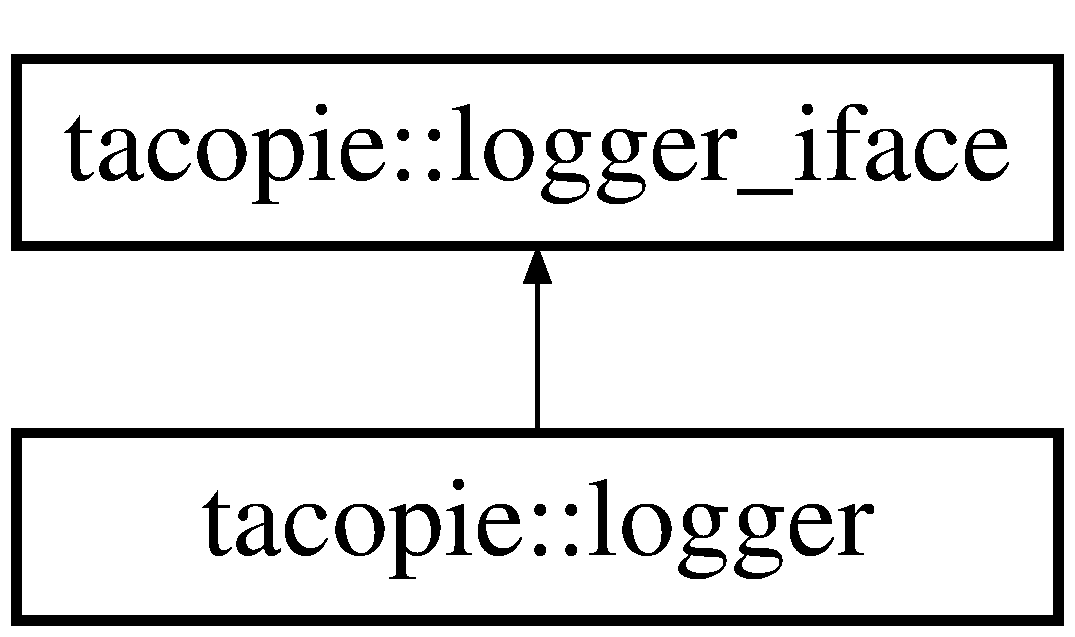
\includegraphics[height=2.000000cm]{classtacopie_1_1logger}
\end{center}
\end{figure}
\subsection*{Public Types}
\begin{DoxyCompactItemize}
\item 
enum \hyperlink{classtacopie_1_1logger_ae7dd235972bbf86a017fc39b3af80efe}{log\+\_\+level} \{ \hyperlink{classtacopie_1_1logger_ae7dd235972bbf86a017fc39b3af80efeacb5e100e5a9a3e7f6d1fd97512215282}{log\+\_\+level\+::error} = 0, 
\hyperlink{classtacopie_1_1logger_ae7dd235972bbf86a017fc39b3af80efea1ea4c3ab05ee0c6d4de30740443769cb}{log\+\_\+level\+::warn} = 1, 
\hyperlink{classtacopie_1_1logger_ae7dd235972bbf86a017fc39b3af80efeacaf9b6b99962bf5c2264824231d7a40c}{log\+\_\+level\+::info} = 2, 
\hyperlink{classtacopie_1_1logger_ae7dd235972bbf86a017fc39b3af80efeaad42f6697b035b7580e4fef93be20b4d}{log\+\_\+level\+::debug} = 3
 \}
\end{DoxyCompactItemize}
\subsection*{Public Member Functions}
\begin{DoxyCompactItemize}
\item 
\hyperlink{classtacopie_1_1logger_af863301c0ef7f646469eb944285cb280}{logger} (\hyperlink{classtacopie_1_1logger_ae7dd235972bbf86a017fc39b3af80efe}{log\+\_\+level} level=\hyperlink{classtacopie_1_1logger_ae7dd235972bbf86a017fc39b3af80efeacaf9b6b99962bf5c2264824231d7a40c}{log\+\_\+level\+::info})
\begin{DoxyCompactList}\small\item\em ctor \end{DoxyCompactList}\item 
\hyperlink{classtacopie_1_1logger_af5c89b85935dbe3b4da3199247d50398}{$\sim$logger} (void)=default
\begin{DoxyCompactList}\small\item\em dtor \end{DoxyCompactList}\item 
\hyperlink{classtacopie_1_1logger_af22e5c126a0e0dbd4c82dc1c40b2d16f}{logger} (const \hyperlink{classtacopie_1_1logger}{logger} \&)=default
\begin{DoxyCompactList}\small\item\em copy ctor \end{DoxyCompactList}\item 
\hyperlink{classtacopie_1_1logger}{logger} \& \hyperlink{classtacopie_1_1logger_a4ee4e53fa0857ee404ddfd5b40759162}{operator=} (const \hyperlink{classtacopie_1_1logger}{logger} \&)=default
\begin{DoxyCompactList}\small\item\em assignment operator \end{DoxyCompactList}\item 
void \hyperlink{classtacopie_1_1logger_aff31bbc7d3fdbbe60a2331fe24ec76ff}{debug} (const std\+::string \&msg, const std\+::string \&file, std\+::size\+\_\+t line)
\item 
void \hyperlink{classtacopie_1_1logger_a5089c5a6127586d4f2ea3a69a0bf6570}{info} (const std\+::string \&msg, const std\+::string \&file, std\+::size\+\_\+t line)
\item 
void \hyperlink{classtacopie_1_1logger_aa4cd2ffc3f4b9d096a35c5c2aa8e0970}{warn} (const std\+::string \&msg, const std\+::string \&file, std\+::size\+\_\+t line)
\item 
void \hyperlink{classtacopie_1_1logger_a3fe1be02ac2f4e4fe44a0bdaf8359546}{error} (const std\+::string \&msg, const std\+::string \&file, std\+::size\+\_\+t line)
\end{DoxyCompactItemize}
\subsection*{Private Attributes}
\begin{DoxyCompactItemize}
\item 
\hyperlink{classtacopie_1_1logger_ae7dd235972bbf86a017fc39b3af80efe}{log\+\_\+level} \hyperlink{classtacopie_1_1logger_ae694159c13994aa03bc578feca597c04}{m\+\_\+level}
\item 
std\+::mutex \hyperlink{classtacopie_1_1logger_ab04fda465e61bc7a84aa456bf2e399b0}{m\+\_\+mutex}
\end{DoxyCompactItemize}


\subsection{Detailed Description}
default logger class provided by the library 

\subsection{Member Enumeration Documentation}
\mbox{\Hypertarget{classtacopie_1_1logger_ae7dd235972bbf86a017fc39b3af80efe}\label{classtacopie_1_1logger_ae7dd235972bbf86a017fc39b3af80efe}} 
\index{tacopie\+::logger@{tacopie\+::logger}!log\+\_\+level@{log\+\_\+level}}
\index{log\+\_\+level@{log\+\_\+level}!tacopie\+::logger@{tacopie\+::logger}}
\subsubsection{\texorpdfstring{log\+\_\+level}{log\_level}}
{\footnotesize\ttfamily enum \hyperlink{classtacopie_1_1logger_ae7dd235972bbf86a017fc39b3af80efe}{tacopie\+::logger\+::log\+\_\+level}\hspace{0.3cm}{\ttfamily [strong]}}

log level \begin{DoxyEnumFields}{Enumerator}
\raisebox{\heightof{T}}[0pt][0pt]{\index{error@{error}!tacopie\+::logger@{tacopie\+::logger}}\index{tacopie\+::logger@{tacopie\+::logger}!error@{error}}}\mbox{\Hypertarget{classtacopie_1_1logger_ae7dd235972bbf86a017fc39b3af80efeacb5e100e5a9a3e7f6d1fd97512215282}\label{classtacopie_1_1logger_ae7dd235972bbf86a017fc39b3af80efeacb5e100e5a9a3e7f6d1fd97512215282}} 
error&\\
\hline

\raisebox{\heightof{T}}[0pt][0pt]{\index{warn@{warn}!tacopie\+::logger@{tacopie\+::logger}}\index{tacopie\+::logger@{tacopie\+::logger}!warn@{warn}}}\mbox{\Hypertarget{classtacopie_1_1logger_ae7dd235972bbf86a017fc39b3af80efea1ea4c3ab05ee0c6d4de30740443769cb}\label{classtacopie_1_1logger_ae7dd235972bbf86a017fc39b3af80efea1ea4c3ab05ee0c6d4de30740443769cb}} 
warn&\\
\hline

\raisebox{\heightof{T}}[0pt][0pt]{\index{info@{info}!tacopie\+::logger@{tacopie\+::logger}}\index{tacopie\+::logger@{tacopie\+::logger}!info@{info}}}\mbox{\Hypertarget{classtacopie_1_1logger_ae7dd235972bbf86a017fc39b3af80efeacaf9b6b99962bf5c2264824231d7a40c}\label{classtacopie_1_1logger_ae7dd235972bbf86a017fc39b3af80efeacaf9b6b99962bf5c2264824231d7a40c}} 
info&\\
\hline

\raisebox{\heightof{T}}[0pt][0pt]{\index{debug@{debug}!tacopie\+::logger@{tacopie\+::logger}}\index{tacopie\+::logger@{tacopie\+::logger}!debug@{debug}}}\mbox{\Hypertarget{classtacopie_1_1logger_ae7dd235972bbf86a017fc39b3af80efeaad42f6697b035b7580e4fef93be20b4d}\label{classtacopie_1_1logger_ae7dd235972bbf86a017fc39b3af80efeaad42f6697b035b7580e4fef93be20b4d}} 
debug&\\
\hline

\end{DoxyEnumFields}


\subsection{Constructor \& Destructor Documentation}
\mbox{\Hypertarget{classtacopie_1_1logger_af863301c0ef7f646469eb944285cb280}\label{classtacopie_1_1logger_af863301c0ef7f646469eb944285cb280}} 
\index{tacopie\+::logger@{tacopie\+::logger}!logger@{logger}}
\index{logger@{logger}!tacopie\+::logger@{tacopie\+::logger}}
\subsubsection{\texorpdfstring{logger()}{logger()}\hspace{0.1cm}{\footnotesize\ttfamily [1/2]}}
{\footnotesize\ttfamily tacopie\+::logger\+::logger (\begin{DoxyParamCaption}\item[{\hyperlink{classtacopie_1_1logger_ae7dd235972bbf86a017fc39b3af80efe}{log\+\_\+level}}]{level = {\ttfamily \hyperlink{classtacopie_1_1logger_ae7dd235972bbf86a017fc39b3af80efeacaf9b6b99962bf5c2264824231d7a40c}{log\+\_\+level\+::info}} }\end{DoxyParamCaption})}



ctor 

\mbox{\Hypertarget{classtacopie_1_1logger_af5c89b85935dbe3b4da3199247d50398}\label{classtacopie_1_1logger_af5c89b85935dbe3b4da3199247d50398}} 
\index{tacopie\+::logger@{tacopie\+::logger}!````~logger@{$\sim$logger}}
\index{````~logger@{$\sim$logger}!tacopie\+::logger@{tacopie\+::logger}}
\subsubsection{\texorpdfstring{$\sim$logger()}{~logger()}}
{\footnotesize\ttfamily tacopie\+::logger\+::$\sim$logger (\begin{DoxyParamCaption}\item[{void}]{ }\end{DoxyParamCaption})\hspace{0.3cm}{\ttfamily [default]}}



dtor 

\mbox{\Hypertarget{classtacopie_1_1logger_af22e5c126a0e0dbd4c82dc1c40b2d16f}\label{classtacopie_1_1logger_af22e5c126a0e0dbd4c82dc1c40b2d16f}} 
\index{tacopie\+::logger@{tacopie\+::logger}!logger@{logger}}
\index{logger@{logger}!tacopie\+::logger@{tacopie\+::logger}}
\subsubsection{\texorpdfstring{logger()}{logger()}\hspace{0.1cm}{\footnotesize\ttfamily [2/2]}}
{\footnotesize\ttfamily tacopie\+::logger\+::logger (\begin{DoxyParamCaption}\item[{const \hyperlink{classtacopie_1_1logger}{logger} \&}]{ }\end{DoxyParamCaption})\hspace{0.3cm}{\ttfamily [default]}}



copy ctor 



\subsection{Member Function Documentation}
\mbox{\Hypertarget{classtacopie_1_1logger_aff31bbc7d3fdbbe60a2331fe24ec76ff}\label{classtacopie_1_1logger_aff31bbc7d3fdbbe60a2331fe24ec76ff}} 
\index{tacopie\+::logger@{tacopie\+::logger}!debug@{debug}}
\index{debug@{debug}!tacopie\+::logger@{tacopie\+::logger}}
\subsubsection{\texorpdfstring{debug()}{debug()}}
{\footnotesize\ttfamily void tacopie\+::logger\+::debug (\begin{DoxyParamCaption}\item[{const std\+::string \&}]{msg,  }\item[{const std\+::string \&}]{file,  }\item[{std\+::size\+\_\+t}]{line }\end{DoxyParamCaption})\hspace{0.3cm}{\ttfamily [virtual]}}

debug logging


\begin{DoxyParams}{Parameters}
{\em msg} & message to be logged \\
\hline
{\em file} & file from which the message is coming \\
\hline
{\em line} & line in the file of the message \\
\hline
\end{DoxyParams}


Implements \hyperlink{classtacopie_1_1logger__iface_a156abb02ab852ea4033fc13f4902ee7a}{tacopie\+::logger\+\_\+iface}.

\mbox{\Hypertarget{classtacopie_1_1logger_a3fe1be02ac2f4e4fe44a0bdaf8359546}\label{classtacopie_1_1logger_a3fe1be02ac2f4e4fe44a0bdaf8359546}} 
\index{tacopie\+::logger@{tacopie\+::logger}!error@{error}}
\index{error@{error}!tacopie\+::logger@{tacopie\+::logger}}
\subsubsection{\texorpdfstring{error()}{error()}}
{\footnotesize\ttfamily void tacopie\+::logger\+::error (\begin{DoxyParamCaption}\item[{const std\+::string \&}]{msg,  }\item[{const std\+::string \&}]{file,  }\item[{std\+::size\+\_\+t}]{line }\end{DoxyParamCaption})\hspace{0.3cm}{\ttfamily [virtual]}}

error logging


\begin{DoxyParams}{Parameters}
{\em msg} & message to be logged \\
\hline
{\em file} & file from which the message is coming \\
\hline
{\em line} & line in the file of the message \\
\hline
\end{DoxyParams}


Implements \hyperlink{classtacopie_1_1logger__iface_a18f9c02fc19be4b9900ac9fb1a361624}{tacopie\+::logger\+\_\+iface}.

\mbox{\Hypertarget{classtacopie_1_1logger_a5089c5a6127586d4f2ea3a69a0bf6570}\label{classtacopie_1_1logger_a5089c5a6127586d4f2ea3a69a0bf6570}} 
\index{tacopie\+::logger@{tacopie\+::logger}!info@{info}}
\index{info@{info}!tacopie\+::logger@{tacopie\+::logger}}
\subsubsection{\texorpdfstring{info()}{info()}}
{\footnotesize\ttfamily void tacopie\+::logger\+::info (\begin{DoxyParamCaption}\item[{const std\+::string \&}]{msg,  }\item[{const std\+::string \&}]{file,  }\item[{std\+::size\+\_\+t}]{line }\end{DoxyParamCaption})\hspace{0.3cm}{\ttfamily [virtual]}}

info logging


\begin{DoxyParams}{Parameters}
{\em msg} & message to be logged \\
\hline
{\em file} & file from which the message is coming \\
\hline
{\em line} & line in the file of the message \\
\hline
\end{DoxyParams}


Implements \hyperlink{classtacopie_1_1logger__iface_af176525bca036944f75bad6469860929}{tacopie\+::logger\+\_\+iface}.

\mbox{\Hypertarget{classtacopie_1_1logger_a4ee4e53fa0857ee404ddfd5b40759162}\label{classtacopie_1_1logger_a4ee4e53fa0857ee404ddfd5b40759162}} 
\index{tacopie\+::logger@{tacopie\+::logger}!operator=@{operator=}}
\index{operator=@{operator=}!tacopie\+::logger@{tacopie\+::logger}}
\subsubsection{\texorpdfstring{operator=()}{operator=()}}
{\footnotesize\ttfamily \hyperlink{classtacopie_1_1logger}{logger}\& tacopie\+::logger\+::operator= (\begin{DoxyParamCaption}\item[{const \hyperlink{classtacopie_1_1logger}{logger} \&}]{ }\end{DoxyParamCaption})\hspace{0.3cm}{\ttfamily [default]}}



assignment operator 

\mbox{\Hypertarget{classtacopie_1_1logger_aa4cd2ffc3f4b9d096a35c5c2aa8e0970}\label{classtacopie_1_1logger_aa4cd2ffc3f4b9d096a35c5c2aa8e0970}} 
\index{tacopie\+::logger@{tacopie\+::logger}!warn@{warn}}
\index{warn@{warn}!tacopie\+::logger@{tacopie\+::logger}}
\subsubsection{\texorpdfstring{warn()}{warn()}}
{\footnotesize\ttfamily void tacopie\+::logger\+::warn (\begin{DoxyParamCaption}\item[{const std\+::string \&}]{msg,  }\item[{const std\+::string \&}]{file,  }\item[{std\+::size\+\_\+t}]{line }\end{DoxyParamCaption})\hspace{0.3cm}{\ttfamily [virtual]}}

warn logging


\begin{DoxyParams}{Parameters}
{\em msg} & message to be logged \\
\hline
{\em file} & file from which the message is coming \\
\hline
{\em line} & line in the file of the message \\
\hline
\end{DoxyParams}


Implements \hyperlink{classtacopie_1_1logger__iface_ab96d8f6bc2e2b514c7ceec4c856f8921}{tacopie\+::logger\+\_\+iface}.



\subsection{Member Data Documentation}
\mbox{\Hypertarget{classtacopie_1_1logger_ae694159c13994aa03bc578feca597c04}\label{classtacopie_1_1logger_ae694159c13994aa03bc578feca597c04}} 
\index{tacopie\+::logger@{tacopie\+::logger}!m\+\_\+level@{m\+\_\+level}}
\index{m\+\_\+level@{m\+\_\+level}!tacopie\+::logger@{tacopie\+::logger}}
\subsubsection{\texorpdfstring{m\+\_\+level}{m\_level}}
{\footnotesize\ttfamily \hyperlink{classtacopie_1_1logger_ae7dd235972bbf86a017fc39b3af80efe}{log\+\_\+level} tacopie\+::logger\+::m\+\_\+level\hspace{0.3cm}{\ttfamily [private]}}

current log level in use \mbox{\Hypertarget{classtacopie_1_1logger_ab04fda465e61bc7a84aa456bf2e399b0}\label{classtacopie_1_1logger_ab04fda465e61bc7a84aa456bf2e399b0}} 
\index{tacopie\+::logger@{tacopie\+::logger}!m\+\_\+mutex@{m\+\_\+mutex}}
\index{m\+\_\+mutex@{m\+\_\+mutex}!tacopie\+::logger@{tacopie\+::logger}}
\subsubsection{\texorpdfstring{m\+\_\+mutex}{m\_mutex}}
{\footnotesize\ttfamily std\+::mutex tacopie\+::logger\+::m\+\_\+mutex\hspace{0.3cm}{\ttfamily [private]}}

mutex used to serialize logs in multithreaded environment 

The documentation for this class was generated from the following file\+:\begin{DoxyCompactItemize}
\item 
includes/tacopie/utils/\hyperlink{logger_8hpp}{logger.\+hpp}\end{DoxyCompactItemize}

\hypertarget{classtacopie_1_1logger__iface}{}\section{tacopie\+:\+:logger\+\_\+iface Class Reference}
\label{classtacopie_1_1logger__iface}\index{tacopie\+::logger\+\_\+iface@{tacopie\+::logger\+\_\+iface}}


{\ttfamily \#include $<$logger.\+hpp$>$}

Inheritance diagram for tacopie\+:\+:logger\+\_\+iface\+:\begin{figure}[H]
\begin{center}
\leavevmode
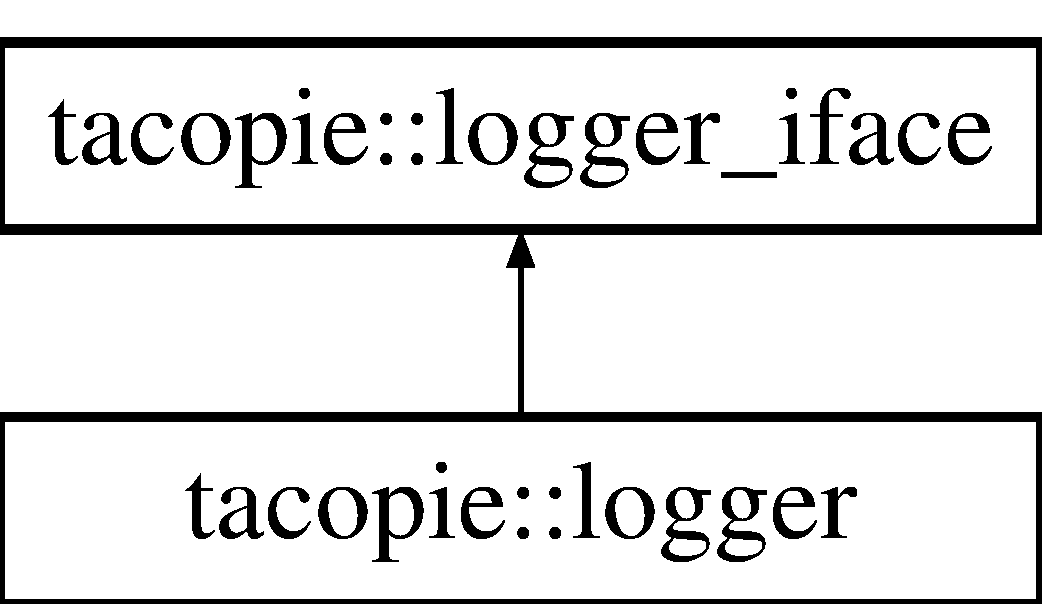
\includegraphics[height=2.000000cm]{classtacopie_1_1logger__iface}
\end{center}
\end{figure}
\subsection*{Public Member Functions}
\begin{DoxyCompactItemize}
\item 
\mbox{\Hypertarget{classtacopie_1_1logger__iface_afccf838f815d168e82e4722e2c4d0d90}\label{classtacopie_1_1logger__iface_afccf838f815d168e82e4722e2c4d0d90}} 
\hyperlink{classtacopie_1_1logger__iface_afccf838f815d168e82e4722e2c4d0d90}{logger\+\_\+iface} (void)=default
\begin{DoxyCompactList}\small\item\em ctor \end{DoxyCompactList}\item 
\mbox{\Hypertarget{classtacopie_1_1logger__iface_a562dcc605198ca90904ba21fa98eb6ea}\label{classtacopie_1_1logger__iface_a562dcc605198ca90904ba21fa98eb6ea}} 
virtual \hyperlink{classtacopie_1_1logger__iface_a562dcc605198ca90904ba21fa98eb6ea}{$\sim$logger\+\_\+iface} (void)=default
\begin{DoxyCompactList}\small\item\em dtor \end{DoxyCompactList}\item 
\mbox{\Hypertarget{classtacopie_1_1logger__iface_a34fb7873b2c5e908afd2d4a0d4965ec1}\label{classtacopie_1_1logger__iface_a34fb7873b2c5e908afd2d4a0d4965ec1}} 
\hyperlink{classtacopie_1_1logger__iface_a34fb7873b2c5e908afd2d4a0d4965ec1}{logger\+\_\+iface} (const \hyperlink{classtacopie_1_1logger__iface}{logger\+\_\+iface} \&)=default
\begin{DoxyCompactList}\small\item\em copy ctor \end{DoxyCompactList}\item 
\mbox{\Hypertarget{classtacopie_1_1logger__iface_ac3ca89b7c5d227b8ed3a5adaa5b72527}\label{classtacopie_1_1logger__iface_ac3ca89b7c5d227b8ed3a5adaa5b72527}} 
\hyperlink{classtacopie_1_1logger__iface}{logger\+\_\+iface} \& \hyperlink{classtacopie_1_1logger__iface_ac3ca89b7c5d227b8ed3a5adaa5b72527}{operator=} (const \hyperlink{classtacopie_1_1logger__iface}{logger\+\_\+iface} \&)=default
\begin{DoxyCompactList}\small\item\em assignment operator \end{DoxyCompactList}\item 
virtual void \hyperlink{classtacopie_1_1logger__iface_a156abb02ab852ea4033fc13f4902ee7a}{debug} (const std\+::string \&msg, const std\+::string \&file, std\+::size\+\_\+t line)=0
\item 
virtual void \hyperlink{classtacopie_1_1logger__iface_af176525bca036944f75bad6469860929}{info} (const std\+::string \&msg, const std\+::string \&file, std\+::size\+\_\+t line)=0
\item 
virtual void \hyperlink{classtacopie_1_1logger__iface_ab96d8f6bc2e2b514c7ceec4c856f8921}{warn} (const std\+::string \&msg, const std\+::string \&file, std\+::size\+\_\+t line)=0
\item 
virtual void \hyperlink{classtacopie_1_1logger__iface_a18f9c02fc19be4b9900ac9fb1a361624}{error} (const std\+::string \&msg, const std\+::string \&file, std\+::size\+\_\+t line)=0
\end{DoxyCompactItemize}


\subsection{Detailed Description}
\hyperlink{classtacopie_1_1logger__iface}{logger\+\_\+iface} should be inherited by any class intended to be used for logging 

\subsection{Member Function Documentation}
\mbox{\Hypertarget{classtacopie_1_1logger__iface_a156abb02ab852ea4033fc13f4902ee7a}\label{classtacopie_1_1logger__iface_a156abb02ab852ea4033fc13f4902ee7a}} 
\index{tacopie\+::logger\+\_\+iface@{tacopie\+::logger\+\_\+iface}!debug@{debug}}
\index{debug@{debug}!tacopie\+::logger\+\_\+iface@{tacopie\+::logger\+\_\+iface}}
\subsubsection{\texorpdfstring{debug()}{debug()}}
{\footnotesize\ttfamily virtual void tacopie\+::logger\+\_\+iface\+::debug (\begin{DoxyParamCaption}\item[{const std\+::string \&}]{msg,  }\item[{const std\+::string \&}]{file,  }\item[{std\+::size\+\_\+t}]{line }\end{DoxyParamCaption})\hspace{0.3cm}{\ttfamily [pure virtual]}}

debug logging


\begin{DoxyParams}{Parameters}
{\em msg} & message to be logged \\
\hline
{\em file} & file from which the message is coming \\
\hline
{\em line} & line in the file of the message \\
\hline
\end{DoxyParams}


Implemented in \hyperlink{classtacopie_1_1logger_aff31bbc7d3fdbbe60a2331fe24ec76ff}{tacopie\+::logger}.

\mbox{\Hypertarget{classtacopie_1_1logger__iface_a18f9c02fc19be4b9900ac9fb1a361624}\label{classtacopie_1_1logger__iface_a18f9c02fc19be4b9900ac9fb1a361624}} 
\index{tacopie\+::logger\+\_\+iface@{tacopie\+::logger\+\_\+iface}!error@{error}}
\index{error@{error}!tacopie\+::logger\+\_\+iface@{tacopie\+::logger\+\_\+iface}}
\subsubsection{\texorpdfstring{error()}{error()}}
{\footnotesize\ttfamily virtual void tacopie\+::logger\+\_\+iface\+::error (\begin{DoxyParamCaption}\item[{const std\+::string \&}]{msg,  }\item[{const std\+::string \&}]{file,  }\item[{std\+::size\+\_\+t}]{line }\end{DoxyParamCaption})\hspace{0.3cm}{\ttfamily [pure virtual]}}

error logging


\begin{DoxyParams}{Parameters}
{\em msg} & message to be logged \\
\hline
{\em file} & file from which the message is coming \\
\hline
{\em line} & line in the file of the message \\
\hline
\end{DoxyParams}


Implemented in \hyperlink{classtacopie_1_1logger_a3fe1be02ac2f4e4fe44a0bdaf8359546}{tacopie\+::logger}.

\mbox{\Hypertarget{classtacopie_1_1logger__iface_af176525bca036944f75bad6469860929}\label{classtacopie_1_1logger__iface_af176525bca036944f75bad6469860929}} 
\index{tacopie\+::logger\+\_\+iface@{tacopie\+::logger\+\_\+iface}!info@{info}}
\index{info@{info}!tacopie\+::logger\+\_\+iface@{tacopie\+::logger\+\_\+iface}}
\subsubsection{\texorpdfstring{info()}{info()}}
{\footnotesize\ttfamily virtual void tacopie\+::logger\+\_\+iface\+::info (\begin{DoxyParamCaption}\item[{const std\+::string \&}]{msg,  }\item[{const std\+::string \&}]{file,  }\item[{std\+::size\+\_\+t}]{line }\end{DoxyParamCaption})\hspace{0.3cm}{\ttfamily [pure virtual]}}

info logging


\begin{DoxyParams}{Parameters}
{\em msg} & message to be logged \\
\hline
{\em file} & file from which the message is coming \\
\hline
{\em line} & line in the file of the message \\
\hline
\end{DoxyParams}


Implemented in \hyperlink{classtacopie_1_1logger_a5089c5a6127586d4f2ea3a69a0bf6570}{tacopie\+::logger}.

\mbox{\Hypertarget{classtacopie_1_1logger__iface_ab96d8f6bc2e2b514c7ceec4c856f8921}\label{classtacopie_1_1logger__iface_ab96d8f6bc2e2b514c7ceec4c856f8921}} 
\index{tacopie\+::logger\+\_\+iface@{tacopie\+::logger\+\_\+iface}!warn@{warn}}
\index{warn@{warn}!tacopie\+::logger\+\_\+iface@{tacopie\+::logger\+\_\+iface}}
\subsubsection{\texorpdfstring{warn()}{warn()}}
{\footnotesize\ttfamily virtual void tacopie\+::logger\+\_\+iface\+::warn (\begin{DoxyParamCaption}\item[{const std\+::string \&}]{msg,  }\item[{const std\+::string \&}]{file,  }\item[{std\+::size\+\_\+t}]{line }\end{DoxyParamCaption})\hspace{0.3cm}{\ttfamily [pure virtual]}}

warn logging


\begin{DoxyParams}{Parameters}
{\em msg} & message to be logged \\
\hline
{\em file} & file from which the message is coming \\
\hline
{\em line} & line in the file of the message \\
\hline
\end{DoxyParams}


Implemented in \hyperlink{classtacopie_1_1logger_aa4cd2ffc3f4b9d096a35c5c2aa8e0970}{tacopie\+::logger}.



The documentation for this class was generated from the following file\+:\begin{DoxyCompactItemize}
\item 
includes/tacopie/utils/logger.\+hpp\end{DoxyCompactItemize}

\hypertarget{structtacopie_1_1tcp__client_1_1read__request}{}\section{tacopie\+:\+:tcp\+\_\+client\+:\+:read\+\_\+request Struct Reference}
\label{structtacopie_1_1tcp__client_1_1read__request}\index{tacopie\+::tcp\+\_\+client\+::read\+\_\+request@{tacopie\+::tcp\+\_\+client\+::read\+\_\+request}}


{\ttfamily \#include $<$tcp\+\_\+client.\+hpp$>$}

\subsection*{Public Attributes}
\begin{DoxyCompactItemize}
\item 
std\+::size\+\_\+t \hyperlink{structtacopie_1_1tcp__client_1_1read__request_ad8b69f61884c60596aface363ca947a3}{size}
\item 
\hyperlink{classtacopie_1_1tcp__client_acdf9dea8bac6c56f7b04ce38b9432322}{async\+\_\+read\+\_\+callback\+\_\+t} \hyperlink{structtacopie_1_1tcp__client_1_1read__request_a3d495e82e38efebf763f595392b0db46}{async\+\_\+read\+\_\+callback}
\end{DoxyCompactItemize}


\subsection{Detailed Description}
structure to store read requests information
\begin{DoxyItemize}
\item size\+: Number of bytes to read
\item async\+\_\+read\+\_\+callback\+: Callback to be called on a read operation completion, even though the operation read less bytes than requested. 
\end{DoxyItemize}

\subsection{Member Data Documentation}
\mbox{\Hypertarget{structtacopie_1_1tcp__client_1_1read__request_a3d495e82e38efebf763f595392b0db46}\label{structtacopie_1_1tcp__client_1_1read__request_a3d495e82e38efebf763f595392b0db46}} 
\index{tacopie\+::tcp\+\_\+client\+::read\+\_\+request@{tacopie\+::tcp\+\_\+client\+::read\+\_\+request}!async\+\_\+read\+\_\+callback@{async\+\_\+read\+\_\+callback}}
\index{async\+\_\+read\+\_\+callback@{async\+\_\+read\+\_\+callback}!tacopie\+::tcp\+\_\+client\+::read\+\_\+request@{tacopie\+::tcp\+\_\+client\+::read\+\_\+request}}
\subsubsection{\texorpdfstring{async\+\_\+read\+\_\+callback}{async\_read\_callback}}
{\footnotesize\ttfamily \hyperlink{classtacopie_1_1tcp__client_acdf9dea8bac6c56f7b04ce38b9432322}{async\+\_\+read\+\_\+callback\+\_\+t} tacopie\+::tcp\+\_\+client\+::read\+\_\+request\+::async\+\_\+read\+\_\+callback}

\mbox{\Hypertarget{structtacopie_1_1tcp__client_1_1read__request_ad8b69f61884c60596aface363ca947a3}\label{structtacopie_1_1tcp__client_1_1read__request_ad8b69f61884c60596aface363ca947a3}} 
\index{tacopie\+::tcp\+\_\+client\+::read\+\_\+request@{tacopie\+::tcp\+\_\+client\+::read\+\_\+request}!size@{size}}
\index{size@{size}!tacopie\+::tcp\+\_\+client\+::read\+\_\+request@{tacopie\+::tcp\+\_\+client\+::read\+\_\+request}}
\subsubsection{\texorpdfstring{size}{size}}
{\footnotesize\ttfamily std\+::size\+\_\+t tacopie\+::tcp\+\_\+client\+::read\+\_\+request\+::size}



The documentation for this struct was generated from the following file\+:\begin{DoxyCompactItemize}
\item 
includes/tacopie/network/\hyperlink{tcp__client_8hpp}{tcp\+\_\+client.\+hpp}\end{DoxyCompactItemize}

\hypertarget{structtacopie_1_1tcp__client_1_1read__result}{}\section{tacopie\+:\+:tcp\+\_\+client\+:\+:read\+\_\+result Struct Reference}
\label{structtacopie_1_1tcp__client_1_1read__result}\index{tacopie\+::tcp\+\_\+client\+::read\+\_\+result@{tacopie\+::tcp\+\_\+client\+::read\+\_\+result}}


{\ttfamily \#include $<$tcp\+\_\+client.\+hpp$>$}

\subsection*{Public Attributes}
\begin{DoxyCompactItemize}
\item 
bool \hyperlink{structtacopie_1_1tcp__client_1_1read__result_a9bb917b8d210159a95655a6f8da8e96e}{success}
\item 
std\+::vector$<$ char $>$ \hyperlink{structtacopie_1_1tcp__client_1_1read__result_a50d22ea3a43d085d88d54bbf59a357dc}{buffer}
\end{DoxyCompactItemize}


\subsection{Detailed Description}
structure to store read requests result
\begin{DoxyItemize}
\item success\+: Whether the read operation has succeeded or not. If false, the client has been disconnected
\item buffer\+: Vector containing the read bytes 
\end{DoxyItemize}

\subsection{Member Data Documentation}
\mbox{\Hypertarget{structtacopie_1_1tcp__client_1_1read__result_a50d22ea3a43d085d88d54bbf59a357dc}\label{structtacopie_1_1tcp__client_1_1read__result_a50d22ea3a43d085d88d54bbf59a357dc}} 
\index{tacopie\+::tcp\+\_\+client\+::read\+\_\+result@{tacopie\+::tcp\+\_\+client\+::read\+\_\+result}!buffer@{buffer}}
\index{buffer@{buffer}!tacopie\+::tcp\+\_\+client\+::read\+\_\+result@{tacopie\+::tcp\+\_\+client\+::read\+\_\+result}}
\subsubsection{\texorpdfstring{buffer}{buffer}}
{\footnotesize\ttfamily std\+::vector$<$char$>$ tacopie\+::tcp\+\_\+client\+::read\+\_\+result\+::buffer}

read bytes \mbox{\Hypertarget{structtacopie_1_1tcp__client_1_1read__result_a9bb917b8d210159a95655a6f8da8e96e}\label{structtacopie_1_1tcp__client_1_1read__result_a9bb917b8d210159a95655a6f8da8e96e}} 
\index{tacopie\+::tcp\+\_\+client\+::read\+\_\+result@{tacopie\+::tcp\+\_\+client\+::read\+\_\+result}!success@{success}}
\index{success@{success}!tacopie\+::tcp\+\_\+client\+::read\+\_\+result@{tacopie\+::tcp\+\_\+client\+::read\+\_\+result}}
\subsubsection{\texorpdfstring{success}{success}}
{\footnotesize\ttfamily bool tacopie\+::tcp\+\_\+client\+::read\+\_\+result\+::success}

whether the operation succeeeded or not 

The documentation for this struct was generated from the following file\+:\begin{DoxyCompactItemize}
\item 
includes/tacopie/network/tcp\+\_\+client.\+hpp\end{DoxyCompactItemize}

\hypertarget{classtacopie_1_1self__pipe}{}\section{tacopie\+:\+:self\+\_\+pipe Class Reference}
\label{classtacopie_1_1self__pipe}\index{tacopie\+::self\+\_\+pipe@{tacopie\+::self\+\_\+pipe}}


{\ttfamily \#include $<$self\+\_\+pipe.\+hpp$>$}

\subsection*{Public Member Functions}
\begin{DoxyCompactItemize}
\item 
\hyperlink{classtacopie_1_1self__pipe_add8d2c43863d1505e6851789ab5d9b97}{self\+\_\+pipe} (void)
\begin{DoxyCompactList}\small\item\em ctor \end{DoxyCompactList}\item 
\hyperlink{classtacopie_1_1self__pipe_a10a6c4b0d67a4a14abea397a05cee54c}{$\sim$self\+\_\+pipe} (void)
\begin{DoxyCompactList}\small\item\em dtor \end{DoxyCompactList}\item 
\hyperlink{classtacopie_1_1self__pipe_a09ffc77b89ad48bc8db6635108c68b6b}{self\+\_\+pipe} (const \hyperlink{classtacopie_1_1self__pipe}{self\+\_\+pipe} \&)=delete
\begin{DoxyCompactList}\small\item\em copy ctor \end{DoxyCompactList}\item 
\hyperlink{classtacopie_1_1self__pipe}{self\+\_\+pipe} \& \hyperlink{classtacopie_1_1self__pipe_a14e0fa3a880b6c9559c087eac480c518}{operator=} (const \hyperlink{classtacopie_1_1self__pipe}{self\+\_\+pipe} \&)=delete
\begin{DoxyCompactList}\small\item\em assignment operator \end{DoxyCompactList}\item 
\hyperlink{namespacetacopie_acce7ad26b2d30156b1e6fa353f727026}{fd\+\_\+t} \hyperlink{classtacopie_1_1self__pipe_a301b416f5f8236a383065b381385b88c}{get\+\_\+read\+\_\+fd} (void) const
\item 
\hyperlink{namespacetacopie_acce7ad26b2d30156b1e6fa353f727026}{fd\+\_\+t} \hyperlink{classtacopie_1_1self__pipe_ab36a4deb45bb408988f26315aedc0d74}{get\+\_\+write\+\_\+fd} (void) const
\item 
void \hyperlink{classtacopie_1_1self__pipe_ade9e0e3d19b8d4d22977935a578d508e}{notify} (void)
\item 
void \hyperlink{classtacopie_1_1self__pipe_a4f55a34bd882d59bdcc73b87222ba3d8}{clr\+\_\+buffer} (void)
\end{DoxyCompactItemize}
\subsection*{Private Attributes}
\begin{DoxyCompactItemize}
\item 
\hyperlink{namespacetacopie_acce7ad26b2d30156b1e6fa353f727026}{fd\+\_\+t} \hyperlink{classtacopie_1_1self__pipe_a3e562cfb5ffdd3a8bc6a7c28eca2b7af}{m\+\_\+fds} \mbox{[}2\mbox{]}
\end{DoxyCompactItemize}


\subsection{Constructor \& Destructor Documentation}
\mbox{\Hypertarget{classtacopie_1_1self__pipe_add8d2c43863d1505e6851789ab5d9b97}\label{classtacopie_1_1self__pipe_add8d2c43863d1505e6851789ab5d9b97}} 
\index{tacopie\+::self\+\_\+pipe@{tacopie\+::self\+\_\+pipe}!self\+\_\+pipe@{self\+\_\+pipe}}
\index{self\+\_\+pipe@{self\+\_\+pipe}!tacopie\+::self\+\_\+pipe@{tacopie\+::self\+\_\+pipe}}
\subsubsection{\texorpdfstring{self\+\_\+pipe()}{self\_pipe()}\hspace{0.1cm}{\footnotesize\ttfamily [1/2]}}
{\footnotesize\ttfamily tacopie\+::self\+\_\+pipe\+::self\+\_\+pipe (\begin{DoxyParamCaption}\item[{void}]{ }\end{DoxyParamCaption})}



ctor 

\mbox{\Hypertarget{classtacopie_1_1self__pipe_a10a6c4b0d67a4a14abea397a05cee54c}\label{classtacopie_1_1self__pipe_a10a6c4b0d67a4a14abea397a05cee54c}} 
\index{tacopie\+::self\+\_\+pipe@{tacopie\+::self\+\_\+pipe}!````~self\+\_\+pipe@{$\sim$self\+\_\+pipe}}
\index{````~self\+\_\+pipe@{$\sim$self\+\_\+pipe}!tacopie\+::self\+\_\+pipe@{tacopie\+::self\+\_\+pipe}}
\subsubsection{\texorpdfstring{$\sim$self\+\_\+pipe()}{~self\_pipe()}}
{\footnotesize\ttfamily tacopie\+::self\+\_\+pipe\+::$\sim$self\+\_\+pipe (\begin{DoxyParamCaption}\item[{void}]{ }\end{DoxyParamCaption})}



dtor 

\mbox{\Hypertarget{classtacopie_1_1self__pipe_a09ffc77b89ad48bc8db6635108c68b6b}\label{classtacopie_1_1self__pipe_a09ffc77b89ad48bc8db6635108c68b6b}} 
\index{tacopie\+::self\+\_\+pipe@{tacopie\+::self\+\_\+pipe}!self\+\_\+pipe@{self\+\_\+pipe}}
\index{self\+\_\+pipe@{self\+\_\+pipe}!tacopie\+::self\+\_\+pipe@{tacopie\+::self\+\_\+pipe}}
\subsubsection{\texorpdfstring{self\+\_\+pipe()}{self\_pipe()}\hspace{0.1cm}{\footnotesize\ttfamily [2/2]}}
{\footnotesize\ttfamily tacopie\+::self\+\_\+pipe\+::self\+\_\+pipe (\begin{DoxyParamCaption}\item[{const \hyperlink{classtacopie_1_1self__pipe}{self\+\_\+pipe} \&}]{ }\end{DoxyParamCaption})\hspace{0.3cm}{\ttfamily [delete]}}



copy ctor 



\subsection{Member Function Documentation}
\mbox{\Hypertarget{classtacopie_1_1self__pipe_a4f55a34bd882d59bdcc73b87222ba3d8}\label{classtacopie_1_1self__pipe_a4f55a34bd882d59bdcc73b87222ba3d8}} 
\index{tacopie\+::self\+\_\+pipe@{tacopie\+::self\+\_\+pipe}!clr\+\_\+buffer@{clr\+\_\+buffer}}
\index{clr\+\_\+buffer@{clr\+\_\+buffer}!tacopie\+::self\+\_\+pipe@{tacopie\+::self\+\_\+pipe}}
\subsubsection{\texorpdfstring{clr\+\_\+buffer()}{clr\_buffer()}}
{\footnotesize\ttfamily void tacopie\+::self\+\_\+pipe\+::clr\+\_\+buffer (\begin{DoxyParamCaption}\item[{void}]{ }\end{DoxyParamCaption})}

clear the pipe (basically read from the pipe) \mbox{\Hypertarget{classtacopie_1_1self__pipe_a301b416f5f8236a383065b381385b88c}\label{classtacopie_1_1self__pipe_a301b416f5f8236a383065b381385b88c}} 
\index{tacopie\+::self\+\_\+pipe@{tacopie\+::self\+\_\+pipe}!get\+\_\+read\+\_\+fd@{get\+\_\+read\+\_\+fd}}
\index{get\+\_\+read\+\_\+fd@{get\+\_\+read\+\_\+fd}!tacopie\+::self\+\_\+pipe@{tacopie\+::self\+\_\+pipe}}
\subsubsection{\texorpdfstring{get\+\_\+read\+\_\+fd()}{get\_read\_fd()}}
{\footnotesize\ttfamily \hyperlink{namespacetacopie_acce7ad26b2d30156b1e6fa353f727026}{fd\+\_\+t} tacopie\+::self\+\_\+pipe\+::get\+\_\+read\+\_\+fd (\begin{DoxyParamCaption}\item[{void}]{ }\end{DoxyParamCaption}) const}

\begin{DoxyReturn}{Returns}
the read fd of the pipe 
\end{DoxyReturn}
\mbox{\Hypertarget{classtacopie_1_1self__pipe_ab36a4deb45bb408988f26315aedc0d74}\label{classtacopie_1_1self__pipe_ab36a4deb45bb408988f26315aedc0d74}} 
\index{tacopie\+::self\+\_\+pipe@{tacopie\+::self\+\_\+pipe}!get\+\_\+write\+\_\+fd@{get\+\_\+write\+\_\+fd}}
\index{get\+\_\+write\+\_\+fd@{get\+\_\+write\+\_\+fd}!tacopie\+::self\+\_\+pipe@{tacopie\+::self\+\_\+pipe}}
\subsubsection{\texorpdfstring{get\+\_\+write\+\_\+fd()}{get\_write\_fd()}}
{\footnotesize\ttfamily \hyperlink{namespacetacopie_acce7ad26b2d30156b1e6fa353f727026}{fd\+\_\+t} tacopie\+::self\+\_\+pipe\+::get\+\_\+write\+\_\+fd (\begin{DoxyParamCaption}\item[{void}]{ }\end{DoxyParamCaption}) const}

\begin{DoxyReturn}{Returns}
the write fd of the pipe 
\end{DoxyReturn}
\mbox{\Hypertarget{classtacopie_1_1self__pipe_ade9e0e3d19b8d4d22977935a578d508e}\label{classtacopie_1_1self__pipe_ade9e0e3d19b8d4d22977935a578d508e}} 
\index{tacopie\+::self\+\_\+pipe@{tacopie\+::self\+\_\+pipe}!notify@{notify}}
\index{notify@{notify}!tacopie\+::self\+\_\+pipe@{tacopie\+::self\+\_\+pipe}}
\subsubsection{\texorpdfstring{notify()}{notify()}}
{\footnotesize\ttfamily void tacopie\+::self\+\_\+pipe\+::notify (\begin{DoxyParamCaption}\item[{void}]{ }\end{DoxyParamCaption})}

notify the self pipe (basically write to the pipe) \mbox{\Hypertarget{classtacopie_1_1self__pipe_a14e0fa3a880b6c9559c087eac480c518}\label{classtacopie_1_1self__pipe_a14e0fa3a880b6c9559c087eac480c518}} 
\index{tacopie\+::self\+\_\+pipe@{tacopie\+::self\+\_\+pipe}!operator=@{operator=}}
\index{operator=@{operator=}!tacopie\+::self\+\_\+pipe@{tacopie\+::self\+\_\+pipe}}
\subsubsection{\texorpdfstring{operator=()}{operator=()}}
{\footnotesize\ttfamily \hyperlink{classtacopie_1_1self__pipe}{self\+\_\+pipe}\& tacopie\+::self\+\_\+pipe\+::operator= (\begin{DoxyParamCaption}\item[{const \hyperlink{classtacopie_1_1self__pipe}{self\+\_\+pipe} \&}]{ }\end{DoxyParamCaption})\hspace{0.3cm}{\ttfamily [delete]}}



assignment operator 



\subsection{Member Data Documentation}
\mbox{\Hypertarget{classtacopie_1_1self__pipe_a3e562cfb5ffdd3a8bc6a7c28eca2b7af}\label{classtacopie_1_1self__pipe_a3e562cfb5ffdd3a8bc6a7c28eca2b7af}} 
\index{tacopie\+::self\+\_\+pipe@{tacopie\+::self\+\_\+pipe}!m\+\_\+fds@{m\+\_\+fds}}
\index{m\+\_\+fds@{m\+\_\+fds}!tacopie\+::self\+\_\+pipe@{tacopie\+::self\+\_\+pipe}}
\subsubsection{\texorpdfstring{m\+\_\+fds}{m\_fds}}
{\footnotesize\ttfamily \hyperlink{namespacetacopie_acce7ad26b2d30156b1e6fa353f727026}{fd\+\_\+t} tacopie\+::self\+\_\+pipe\+::m\+\_\+fds\mbox{[}2\mbox{]}\hspace{0.3cm}{\ttfamily [private]}}

pipe file descriptors 

The documentation for this class was generated from the following file\+:\begin{DoxyCompactItemize}
\item 
includes/tacopie/network/\hyperlink{self__pipe_8hpp}{self\+\_\+pipe.\+hpp}\end{DoxyCompactItemize}

\hypertarget{classtacopie_1_1tacopie__error}{}\section{tacopie\+:\+:tacopie\+\_\+error Class Reference}
\label{classtacopie_1_1tacopie__error}\index{tacopie\+::tacopie\+\_\+error@{tacopie\+::tacopie\+\_\+error}}


{\ttfamily \#include $<$error.\+hpp$>$}

Inheritance diagram for tacopie\+:\+:tacopie\+\_\+error\+:\begin{figure}[H]
\begin{center}
\leavevmode
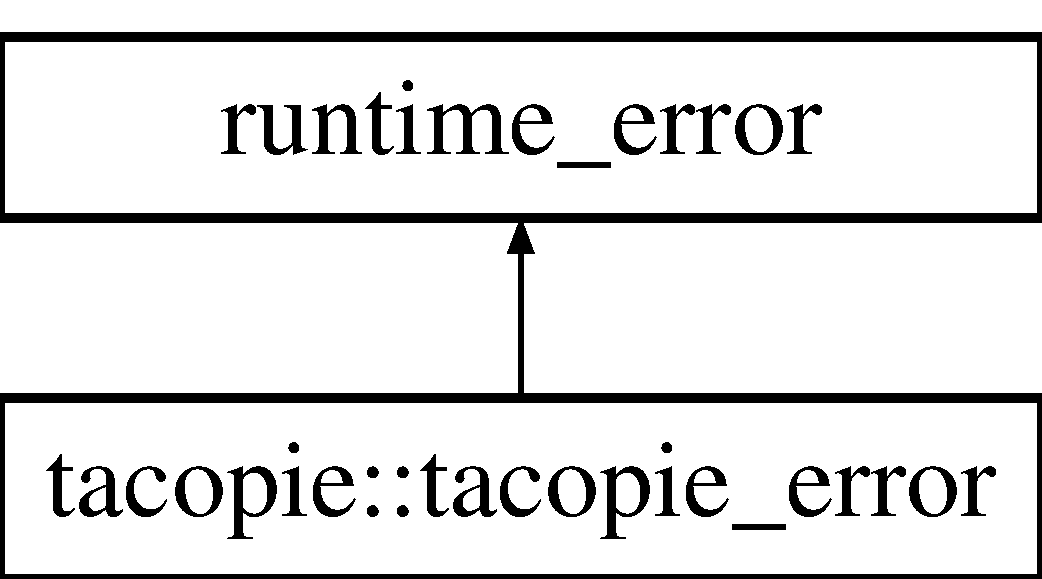
\includegraphics[height=2.000000cm]{classtacopie_1_1tacopie__error}
\end{center}
\end{figure}
\subsection*{Public Member Functions}
\begin{DoxyCompactItemize}
\item 
\hyperlink{classtacopie_1_1tacopie__error_a524fb8e9ac1825a57664421a3f32b9ce}{tacopie\+\_\+error} (const std\+::string \&what, const std\+::string \&file, std\+::size\+\_\+t line)
\begin{DoxyCompactList}\small\item\em ctor \end{DoxyCompactList}\item 
\hyperlink{classtacopie_1_1tacopie__error_a5bf6b0967f7f4cf2b8f8d0a2ef0912b2}{$\sim$tacopie\+\_\+error} (void)=default
\begin{DoxyCompactList}\small\item\em assignment operator \end{DoxyCompactList}\item 
\hyperlink{classtacopie_1_1tacopie__error_a0cb2a911165e08818ca03308891633e1}{tacopie\+\_\+error} (const \hyperlink{classtacopie_1_1tacopie__error}{tacopie\+\_\+error} \&)=default
\begin{DoxyCompactList}\small\item\em copy ctor \end{DoxyCompactList}\item 
\hyperlink{classtacopie_1_1tacopie__error}{tacopie\+\_\+error} \& \hyperlink{classtacopie_1_1tacopie__error_ad30ae4932d33b460f75570f5f3a6e3f3}{operator=} (const \hyperlink{classtacopie_1_1tacopie__error}{tacopie\+\_\+error} \&)=default
\begin{DoxyCompactList}\small\item\em assignment operator \end{DoxyCompactList}\item 
const std\+::string \& \hyperlink{classtacopie_1_1tacopie__error_a10360163c780a1bd9c95fcecca5aa6da}{get\+\_\+file} (void) const
\item 
std\+::size\+\_\+t \hyperlink{classtacopie_1_1tacopie__error_a39704d2cb6f076aa47d45f53f174b257}{get\+\_\+line} (void) const
\end{DoxyCompactItemize}
\subsection*{Private Attributes}
\begin{DoxyCompactItemize}
\item 
std\+::string \hyperlink{classtacopie_1_1tacopie__error_a34c06192d25e3c78b1aed8b0c2ead413}{m\+\_\+file}
\item 
std\+::size\+\_\+t \hyperlink{classtacopie_1_1tacopie__error_a1631d3a1ba6d610e6c6ab0ddaf70b354}{m\+\_\+line}
\end{DoxyCompactItemize}


\subsection{Detailed Description}
specialized runtime\+\_\+error used for tacopie error 

\subsection{Constructor \& Destructor Documentation}
\mbox{\Hypertarget{classtacopie_1_1tacopie__error_a524fb8e9ac1825a57664421a3f32b9ce}\label{classtacopie_1_1tacopie__error_a524fb8e9ac1825a57664421a3f32b9ce}} 
\index{tacopie\+::tacopie\+\_\+error@{tacopie\+::tacopie\+\_\+error}!tacopie\+\_\+error@{tacopie\+\_\+error}}
\index{tacopie\+\_\+error@{tacopie\+\_\+error}!tacopie\+::tacopie\+\_\+error@{tacopie\+::tacopie\+\_\+error}}
\subsubsection{\texorpdfstring{tacopie\+\_\+error()}{tacopie\_error()}\hspace{0.1cm}{\footnotesize\ttfamily [1/2]}}
{\footnotesize\ttfamily tacopie\+::tacopie\+\_\+error\+::tacopie\+\_\+error (\begin{DoxyParamCaption}\item[{const std\+::string \&}]{what,  }\item[{const std\+::string \&}]{file,  }\item[{std\+::size\+\_\+t}]{line }\end{DoxyParamCaption})}



ctor 

\mbox{\Hypertarget{classtacopie_1_1tacopie__error_a5bf6b0967f7f4cf2b8f8d0a2ef0912b2}\label{classtacopie_1_1tacopie__error_a5bf6b0967f7f4cf2b8f8d0a2ef0912b2}} 
\index{tacopie\+::tacopie\+\_\+error@{tacopie\+::tacopie\+\_\+error}!````~tacopie\+\_\+error@{$\sim$tacopie\+\_\+error}}
\index{````~tacopie\+\_\+error@{$\sim$tacopie\+\_\+error}!tacopie\+::tacopie\+\_\+error@{tacopie\+::tacopie\+\_\+error}}
\subsubsection{\texorpdfstring{$\sim$tacopie\+\_\+error()}{~tacopie\_error()}}
{\footnotesize\ttfamily tacopie\+::tacopie\+\_\+error\+::$\sim$tacopie\+\_\+error (\begin{DoxyParamCaption}\item[{void}]{ }\end{DoxyParamCaption})\hspace{0.3cm}{\ttfamily [default]}}



assignment operator 

\mbox{\Hypertarget{classtacopie_1_1tacopie__error_a0cb2a911165e08818ca03308891633e1}\label{classtacopie_1_1tacopie__error_a0cb2a911165e08818ca03308891633e1}} 
\index{tacopie\+::tacopie\+\_\+error@{tacopie\+::tacopie\+\_\+error}!tacopie\+\_\+error@{tacopie\+\_\+error}}
\index{tacopie\+\_\+error@{tacopie\+\_\+error}!tacopie\+::tacopie\+\_\+error@{tacopie\+::tacopie\+\_\+error}}
\subsubsection{\texorpdfstring{tacopie\+\_\+error()}{tacopie\_error()}\hspace{0.1cm}{\footnotesize\ttfamily [2/2]}}
{\footnotesize\ttfamily tacopie\+::tacopie\+\_\+error\+::tacopie\+\_\+error (\begin{DoxyParamCaption}\item[{const \hyperlink{classtacopie_1_1tacopie__error}{tacopie\+\_\+error} \&}]{ }\end{DoxyParamCaption})\hspace{0.3cm}{\ttfamily [default]}}



copy ctor 



\subsection{Member Function Documentation}
\mbox{\Hypertarget{classtacopie_1_1tacopie__error_a10360163c780a1bd9c95fcecca5aa6da}\label{classtacopie_1_1tacopie__error_a10360163c780a1bd9c95fcecca5aa6da}} 
\index{tacopie\+::tacopie\+\_\+error@{tacopie\+::tacopie\+\_\+error}!get\+\_\+file@{get\+\_\+file}}
\index{get\+\_\+file@{get\+\_\+file}!tacopie\+::tacopie\+\_\+error@{tacopie\+::tacopie\+\_\+error}}
\subsubsection{\texorpdfstring{get\+\_\+file()}{get\_file()}}
{\footnotesize\ttfamily const std\+::string\& tacopie\+::tacopie\+\_\+error\+::get\+\_\+file (\begin{DoxyParamCaption}\item[{void}]{ }\end{DoxyParamCaption}) const}

\begin{DoxyReturn}{Returns}
file in which error occured 
\end{DoxyReturn}
\mbox{\Hypertarget{classtacopie_1_1tacopie__error_a39704d2cb6f076aa47d45f53f174b257}\label{classtacopie_1_1tacopie__error_a39704d2cb6f076aa47d45f53f174b257}} 
\index{tacopie\+::tacopie\+\_\+error@{tacopie\+::tacopie\+\_\+error}!get\+\_\+line@{get\+\_\+line}}
\index{get\+\_\+line@{get\+\_\+line}!tacopie\+::tacopie\+\_\+error@{tacopie\+::tacopie\+\_\+error}}
\subsubsection{\texorpdfstring{get\+\_\+line()}{get\_line()}}
{\footnotesize\ttfamily std\+::size\+\_\+t tacopie\+::tacopie\+\_\+error\+::get\+\_\+line (\begin{DoxyParamCaption}\item[{void}]{ }\end{DoxyParamCaption}) const}

\begin{DoxyReturn}{Returns}
line at which the error occured 
\end{DoxyReturn}
\mbox{\Hypertarget{classtacopie_1_1tacopie__error_ad30ae4932d33b460f75570f5f3a6e3f3}\label{classtacopie_1_1tacopie__error_ad30ae4932d33b460f75570f5f3a6e3f3}} 
\index{tacopie\+::tacopie\+\_\+error@{tacopie\+::tacopie\+\_\+error}!operator=@{operator=}}
\index{operator=@{operator=}!tacopie\+::tacopie\+\_\+error@{tacopie\+::tacopie\+\_\+error}}
\subsubsection{\texorpdfstring{operator=()}{operator=()}}
{\footnotesize\ttfamily \hyperlink{classtacopie_1_1tacopie__error}{tacopie\+\_\+error}\& tacopie\+::tacopie\+\_\+error\+::operator= (\begin{DoxyParamCaption}\item[{const \hyperlink{classtacopie_1_1tacopie__error}{tacopie\+\_\+error} \&}]{ }\end{DoxyParamCaption})\hspace{0.3cm}{\ttfamily [default]}}



assignment operator 



\subsection{Member Data Documentation}
\mbox{\Hypertarget{classtacopie_1_1tacopie__error_a34c06192d25e3c78b1aed8b0c2ead413}\label{classtacopie_1_1tacopie__error_a34c06192d25e3c78b1aed8b0c2ead413}} 
\index{tacopie\+::tacopie\+\_\+error@{tacopie\+::tacopie\+\_\+error}!m\+\_\+file@{m\+\_\+file}}
\index{m\+\_\+file@{m\+\_\+file}!tacopie\+::tacopie\+\_\+error@{tacopie\+::tacopie\+\_\+error}}
\subsubsection{\texorpdfstring{m\+\_\+file}{m\_file}}
{\footnotesize\ttfamily std\+::string tacopie\+::tacopie\+\_\+error\+::m\+\_\+file\hspace{0.3cm}{\ttfamily [private]}}

file location of the error \mbox{\Hypertarget{classtacopie_1_1tacopie__error_a1631d3a1ba6d610e6c6ab0ddaf70b354}\label{classtacopie_1_1tacopie__error_a1631d3a1ba6d610e6c6ab0ddaf70b354}} 
\index{tacopie\+::tacopie\+\_\+error@{tacopie\+::tacopie\+\_\+error}!m\+\_\+line@{m\+\_\+line}}
\index{m\+\_\+line@{m\+\_\+line}!tacopie\+::tacopie\+\_\+error@{tacopie\+::tacopie\+\_\+error}}
\subsubsection{\texorpdfstring{m\+\_\+line}{m\_line}}
{\footnotesize\ttfamily std\+::size\+\_\+t tacopie\+::tacopie\+\_\+error\+::m\+\_\+line\hspace{0.3cm}{\ttfamily [private]}}

line location of the error 

The documentation for this class was generated from the following file\+:\begin{DoxyCompactItemize}
\item 
includes/tacopie/utils/\hyperlink{error_8hpp}{error.\+hpp}\end{DoxyCompactItemize}

\hypertarget{classtacopie_1_1tcp__client}{}\section{tacopie\+:\+:tcp\+\_\+client Class Reference}
\label{classtacopie_1_1tcp__client}\index{tacopie\+::tcp\+\_\+client@{tacopie\+::tcp\+\_\+client}}


{\ttfamily \#include $<$tcp\+\_\+client.\+hpp$>$}

\subsection*{Classes}
\begin{DoxyCompactItemize}
\item 
struct \hyperlink{structtacopie_1_1tcp__client_1_1read__request}{read\+\_\+request}
\item 
struct \hyperlink{structtacopie_1_1tcp__client_1_1read__result}{read\+\_\+result}
\item 
struct \hyperlink{structtacopie_1_1tcp__client_1_1write__request}{write\+\_\+request}
\item 
struct \hyperlink{structtacopie_1_1tcp__client_1_1write__result}{write\+\_\+result}
\end{DoxyCompactItemize}
\subsection*{Public Types}
\begin{DoxyCompactItemize}
\item 
typedef std\+::function$<$ void(\hyperlink{structtacopie_1_1tcp__client_1_1read__result}{read\+\_\+result} \&)$>$ \hyperlink{classtacopie_1_1tcp__client_acdf9dea8bac6c56f7b04ce38b9432322}{async\+\_\+read\+\_\+callback\+\_\+t}
\item 
typedef std\+::function$<$ void(\hyperlink{structtacopie_1_1tcp__client_1_1write__result}{write\+\_\+result} \&)$>$ \hyperlink{classtacopie_1_1tcp__client_ad48b8c8dff8a77490eb2e3e802c82b97}{async\+\_\+write\+\_\+callback\+\_\+t}
\item 
typedef std\+::function$<$ void()$>$ \hyperlink{classtacopie_1_1tcp__client_aca5df52e5ee6fa673cf212532ada1453}{disconnection\+\_\+handler\+\_\+t}
\end{DoxyCompactItemize}
\subsection*{Public Member Functions}
\begin{DoxyCompactItemize}
\item 
\hyperlink{classtacopie_1_1tcp__client_a0125e1cf017b0ba0370d682d4382d37b}{tcp\+\_\+client} (std\+::uint32\+\_\+t num\+\_\+io\+\_\+workers=1)
\begin{DoxyCompactList}\small\item\em ctor \& dtor \end{DoxyCompactList}\item 
\hyperlink{classtacopie_1_1tcp__client_ae58e13ec11ab68e3b9e1af2f96933a64}{$\sim$tcp\+\_\+client} (void)
\item 
\hyperlink{classtacopie_1_1tcp__client_a773fbcbb5b79324c8d065e363de73282}{tcp\+\_\+client} (\hyperlink{classtacopie_1_1tcp__socket}{tcp\+\_\+socket} \&\&socket)
\item 
\hyperlink{classtacopie_1_1tcp__client_a5e326782c52f63814cc8f42a901ffaf6}{tcp\+\_\+client} (const \hyperlink{classtacopie_1_1tcp__client}{tcp\+\_\+client} \&)=delete
\begin{DoxyCompactList}\small\item\em copy ctor \end{DoxyCompactList}\item 
\hyperlink{classtacopie_1_1tcp__client}{tcp\+\_\+client} \& \hyperlink{classtacopie_1_1tcp__client_aeadcfb8cd727b2917ebcd357311d0a6b}{operator=} (const \hyperlink{classtacopie_1_1tcp__client}{tcp\+\_\+client} \&)=delete
\begin{DoxyCompactList}\small\item\em assignment operator \end{DoxyCompactList}\item 
bool \hyperlink{classtacopie_1_1tcp__client_af7a1796c04efd00542349ecab692e073}{operator==} (const \hyperlink{classtacopie_1_1tcp__client}{tcp\+\_\+client} \&rhs) const
\item 
bool \hyperlink{classtacopie_1_1tcp__client_af352b6b1e939c919aec2761517051eb9}{operator!=} (const \hyperlink{classtacopie_1_1tcp__client}{tcp\+\_\+client} \&rhs) const
\item 
const std\+::string \& \hyperlink{classtacopie_1_1tcp__client_ad38ab710c5eca64de2f887abc455b15d}{get\+\_\+host} (void) const
\item 
std\+::uint32\+\_\+t \hyperlink{classtacopie_1_1tcp__client_a3b42ae2afe6d5ee5f2f16b8bd7846f37}{get\+\_\+port} (void) const
\item 
void \hyperlink{classtacopie_1_1tcp__client_a0cfbb18cb72aa3b6a41921f61cacc425}{connect} (const std\+::string \&host, std\+::uint32\+\_\+t port, std\+::uint32\+\_\+t timeout\+\_\+msecs=0)
\item 
void \hyperlink{classtacopie_1_1tcp__client_a7562e0bfa24912595d6f695f848b9e51}{disconnect} (bool wait\+\_\+for\+\_\+removal=false)
\item 
bool \hyperlink{classtacopie_1_1tcp__client_a9bf568812c8350260843842e7952c8c3}{is\+\_\+connected} (void) const
\item 
void \hyperlink{classtacopie_1_1tcp__client_a120e3ec2902acc902f7a0b27074bda6b}{async\+\_\+read} (const \hyperlink{structtacopie_1_1tcp__client_1_1read__request}{read\+\_\+request} \&request)
\item 
void \hyperlink{classtacopie_1_1tcp__client_a2304ed6d4ca0cbc74e6aa72d3e92b76a}{async\+\_\+write} (const \hyperlink{structtacopie_1_1tcp__client_1_1write__request}{write\+\_\+request} \&request)
\item 
\hyperlink{classtacopie_1_1tcp__socket}{tacopie\+::tcp\+\_\+socket} \& \hyperlink{classtacopie_1_1tcp__client_a1a3834deb1d263ec5816066f74286298}{get\+\_\+socket} (void)
\item 
const \hyperlink{classtacopie_1_1tcp__socket}{tacopie\+::tcp\+\_\+socket} \& \hyperlink{classtacopie_1_1tcp__client_a9cf1f3ccf43f9a0a883a17b15e3668d6}{get\+\_\+socket} (void) const
\item 
const std\+::shared\+\_\+ptr$<$ \hyperlink{classtacopie_1_1io__service}{tacopie\+::io\+\_\+service} $>$ \& \hyperlink{classtacopie_1_1tcp__client_aafbf0aa37cd0472778d09fb163362314}{get\+\_\+io\+\_\+service} (void) const
\item 
void \hyperlink{classtacopie_1_1tcp__client_a8c290d681186edb0578051c04f3c0762}{set\+\_\+on\+\_\+disconnection\+\_\+handler} (const \hyperlink{classtacopie_1_1tcp__client_aca5df52e5ee6fa673cf212532ada1453}{disconnection\+\_\+handler\+\_\+t} \&disconnection\+\_\+handler)
\end{DoxyCompactItemize}
\subsection*{Private Member Functions}
\begin{DoxyCompactItemize}
\item 
void \hyperlink{classtacopie_1_1tcp__client_ae38ae1f64909dd36592a02fc3c245672}{call\+\_\+disconnection\+\_\+handler} (void)
\item 
void \hyperlink{classtacopie_1_1tcp__client_acb08202e4ea7d85df4a6959dfe418eba}{on\+\_\+read\+\_\+available} (\hyperlink{namespacetacopie_acce7ad26b2d30156b1e6fa353f727026}{fd\+\_\+t} fd)
\item 
void \hyperlink{classtacopie_1_1tcp__client_aee290ddef8906d49edf3bdc9e3555d0a}{on\+\_\+write\+\_\+available} (\hyperlink{namespacetacopie_acce7ad26b2d30156b1e6fa353f727026}{fd\+\_\+t} fd)
\item 
void \hyperlink{classtacopie_1_1tcp__client_afdb370d07800a95448a645f4605d54e1}{clear\+\_\+read\+\_\+requests} (void)
\item 
void \hyperlink{classtacopie_1_1tcp__client_acd8c8d54f359ed99be3a2dd50ef0ec77}{clear\+\_\+write\+\_\+requests} (void)
\item 
\hyperlink{classtacopie_1_1tcp__client_acdf9dea8bac6c56f7b04ce38b9432322}{async\+\_\+read\+\_\+callback\+\_\+t} \hyperlink{classtacopie_1_1tcp__client_a40308b6a1642a79a35a2b2d9c9b9a3f7}{process\+\_\+read} (\hyperlink{structtacopie_1_1tcp__client_1_1read__result}{read\+\_\+result} \&result)
\item 
\hyperlink{classtacopie_1_1tcp__client_ad48b8c8dff8a77490eb2e3e802c82b97}{async\+\_\+write\+\_\+callback\+\_\+t} \hyperlink{classtacopie_1_1tcp__client_afd5e43d5f44930894de10ce05268607f}{process\+\_\+write} (\hyperlink{structtacopie_1_1tcp__client_1_1write__result}{write\+\_\+result} \&result)
\end{DoxyCompactItemize}
\subsection*{Private Attributes}
\begin{DoxyCompactItemize}
\item 
std\+::shared\+\_\+ptr$<$ \hyperlink{classtacopie_1_1io__service}{io\+\_\+service} $>$ \hyperlink{classtacopie_1_1tcp__client_a2a5e4ae0f4fbcd375df4cb1f8070b993}{m\+\_\+io\+\_\+service}
\item 
\hyperlink{classtacopie_1_1tcp__socket}{tacopie\+::tcp\+\_\+socket} \hyperlink{classtacopie_1_1tcp__client_ad256815911a745fce8f2aed00fb45b21}{m\+\_\+socket}
\item 
std\+::atomic$<$ bool $>$ \hyperlink{classtacopie_1_1tcp__client_adf45ef6f910a7723fcfe543417f1feaf}{m\+\_\+is\+\_\+connected} = A\+T\+O\+M\+I\+C\+\_\+\+V\+A\+R\+\_\+\+I\+N\+IT(false)
\item 
std\+::queue$<$ \hyperlink{structtacopie_1_1tcp__client_1_1read__request}{read\+\_\+request} $>$ \hyperlink{classtacopie_1_1tcp__client_a458754e266c0f41b42e17806cc59dc2a}{m\+\_\+read\+\_\+requests}
\item 
std\+::queue$<$ \hyperlink{structtacopie_1_1tcp__client_1_1write__request}{write\+\_\+request} $>$ \hyperlink{classtacopie_1_1tcp__client_aabf49a27ada2707f252b295dcec13969}{m\+\_\+write\+\_\+requests}
\item 
std\+::mutex \hyperlink{classtacopie_1_1tcp__client_a792be0da277e372460fbe6977f03d27b}{m\+\_\+read\+\_\+requests\+\_\+mtx}
\item 
std\+::mutex \hyperlink{classtacopie_1_1tcp__client_abc7c664a73d528c0b1c226d35f7bae2f}{m\+\_\+write\+\_\+requests\+\_\+mtx}
\item 
\hyperlink{classtacopie_1_1tcp__client_aca5df52e5ee6fa673cf212532ada1453}{disconnection\+\_\+handler\+\_\+t} \hyperlink{classtacopie_1_1tcp__client_a5ee7259fe6a8258515162e1ed516de20}{m\+\_\+disconnection\+\_\+handler}
\end{DoxyCompactItemize}


\subsection{Member Typedef Documentation}
\mbox{\Hypertarget{classtacopie_1_1tcp__client_acdf9dea8bac6c56f7b04ce38b9432322}\label{classtacopie_1_1tcp__client_acdf9dea8bac6c56f7b04ce38b9432322}} 
\index{tacopie\+::tcp\+\_\+client@{tacopie\+::tcp\+\_\+client}!async\+\_\+read\+\_\+callback\+\_\+t@{async\+\_\+read\+\_\+callback\+\_\+t}}
\index{async\+\_\+read\+\_\+callback\+\_\+t@{async\+\_\+read\+\_\+callback\+\_\+t}!tacopie\+::tcp\+\_\+client@{tacopie\+::tcp\+\_\+client}}
\subsubsection{\texorpdfstring{async\+\_\+read\+\_\+callback\+\_\+t}{async\_read\_callback\_t}}
{\footnotesize\ttfamily typedef std\+::function$<$void(\hyperlink{structtacopie_1_1tcp__client_1_1read__result}{read\+\_\+result}\&)$>$ \hyperlink{classtacopie_1_1tcp__client_acdf9dea8bac6c56f7b04ce38b9432322}{tacopie\+::tcp\+\_\+client\+::async\+\_\+read\+\_\+callback\+\_\+t}}

callback to be called on async read completion takes the \hyperlink{structtacopie_1_1tcp__client_1_1read__result}{read\+\_\+result} as a parameter \mbox{\Hypertarget{classtacopie_1_1tcp__client_ad48b8c8dff8a77490eb2e3e802c82b97}\label{classtacopie_1_1tcp__client_ad48b8c8dff8a77490eb2e3e802c82b97}} 
\index{tacopie\+::tcp\+\_\+client@{tacopie\+::tcp\+\_\+client}!async\+\_\+write\+\_\+callback\+\_\+t@{async\+\_\+write\+\_\+callback\+\_\+t}}
\index{async\+\_\+write\+\_\+callback\+\_\+t@{async\+\_\+write\+\_\+callback\+\_\+t}!tacopie\+::tcp\+\_\+client@{tacopie\+::tcp\+\_\+client}}
\subsubsection{\texorpdfstring{async\+\_\+write\+\_\+callback\+\_\+t}{async\_write\_callback\_t}}
{\footnotesize\ttfamily typedef std\+::function$<$void(\hyperlink{structtacopie_1_1tcp__client_1_1write__result}{write\+\_\+result}\&)$>$ \hyperlink{classtacopie_1_1tcp__client_ad48b8c8dff8a77490eb2e3e802c82b97}{tacopie\+::tcp\+\_\+client\+::async\+\_\+write\+\_\+callback\+\_\+t}}

callback to be called on async write completion takes the \hyperlink{structtacopie_1_1tcp__client_1_1write__result}{write\+\_\+result} as a parameter \mbox{\Hypertarget{classtacopie_1_1tcp__client_aca5df52e5ee6fa673cf212532ada1453}\label{classtacopie_1_1tcp__client_aca5df52e5ee6fa673cf212532ada1453}} 
\index{tacopie\+::tcp\+\_\+client@{tacopie\+::tcp\+\_\+client}!disconnection\+\_\+handler\+\_\+t@{disconnection\+\_\+handler\+\_\+t}}
\index{disconnection\+\_\+handler\+\_\+t@{disconnection\+\_\+handler\+\_\+t}!tacopie\+::tcp\+\_\+client@{tacopie\+::tcp\+\_\+client}}
\subsubsection{\texorpdfstring{disconnection\+\_\+handler\+\_\+t}{disconnection\_handler\_t}}
{\footnotesize\ttfamily typedef std\+::function$<$void()$>$ \hyperlink{classtacopie_1_1tcp__client_aca5df52e5ee6fa673cf212532ada1453}{tacopie\+::tcp\+\_\+client\+::disconnection\+\_\+handler\+\_\+t}}

disconnection handle called whenever a disconnection occured 

\subsection{Constructor \& Destructor Documentation}
\mbox{\Hypertarget{classtacopie_1_1tcp__client_a0125e1cf017b0ba0370d682d4382d37b}\label{classtacopie_1_1tcp__client_a0125e1cf017b0ba0370d682d4382d37b}} 
\index{tacopie\+::tcp\+\_\+client@{tacopie\+::tcp\+\_\+client}!tcp\+\_\+client@{tcp\+\_\+client}}
\index{tcp\+\_\+client@{tcp\+\_\+client}!tacopie\+::tcp\+\_\+client@{tacopie\+::tcp\+\_\+client}}
\subsubsection{\texorpdfstring{tcp\+\_\+client()}{tcp\_client()}\hspace{0.1cm}{\footnotesize\ttfamily [1/3]}}
{\footnotesize\ttfamily tacopie\+::tcp\+\_\+client\+::tcp\+\_\+client (\begin{DoxyParamCaption}\item[{std\+::uint32\+\_\+t}]{num\+\_\+io\+\_\+workers = {\ttfamily 1} }\end{DoxyParamCaption})}



ctor \& dtor 

\mbox{\Hypertarget{classtacopie_1_1tcp__client_ae58e13ec11ab68e3b9e1af2f96933a64}\label{classtacopie_1_1tcp__client_ae58e13ec11ab68e3b9e1af2f96933a64}} 
\index{tacopie\+::tcp\+\_\+client@{tacopie\+::tcp\+\_\+client}!````~tcp\+\_\+client@{$\sim$tcp\+\_\+client}}
\index{````~tcp\+\_\+client@{$\sim$tcp\+\_\+client}!tacopie\+::tcp\+\_\+client@{tacopie\+::tcp\+\_\+client}}
\subsubsection{\texorpdfstring{$\sim$tcp\+\_\+client()}{~tcp\_client()}}
{\footnotesize\ttfamily tacopie\+::tcp\+\_\+client\+::$\sim$tcp\+\_\+client (\begin{DoxyParamCaption}\item[{void}]{ }\end{DoxyParamCaption})}

\mbox{\Hypertarget{classtacopie_1_1tcp__client_a773fbcbb5b79324c8d065e363de73282}\label{classtacopie_1_1tcp__client_a773fbcbb5b79324c8d065e363de73282}} 
\index{tacopie\+::tcp\+\_\+client@{tacopie\+::tcp\+\_\+client}!tcp\+\_\+client@{tcp\+\_\+client}}
\index{tcp\+\_\+client@{tcp\+\_\+client}!tacopie\+::tcp\+\_\+client@{tacopie\+::tcp\+\_\+client}}
\subsubsection{\texorpdfstring{tcp\+\_\+client()}{tcp\_client()}\hspace{0.1cm}{\footnotesize\ttfamily [2/3]}}
{\footnotesize\ttfamily tacopie\+::tcp\+\_\+client\+::tcp\+\_\+client (\begin{DoxyParamCaption}\item[{\hyperlink{classtacopie_1_1tcp__socket}{tcp\+\_\+socket} \&\&}]{socket }\end{DoxyParamCaption})\hspace{0.3cm}{\ttfamily [explicit]}}

custom ctor build socket from existing socket


\begin{DoxyParams}{Parameters}
{\em socket} & \hyperlink{classtacopie_1_1tcp__socket}{tcp\+\_\+socket} instance to be used for building the client (socket will be moved) \\
\hline
\end{DoxyParams}
\mbox{\Hypertarget{classtacopie_1_1tcp__client_a5e326782c52f63814cc8f42a901ffaf6}\label{classtacopie_1_1tcp__client_a5e326782c52f63814cc8f42a901ffaf6}} 
\index{tacopie\+::tcp\+\_\+client@{tacopie\+::tcp\+\_\+client}!tcp\+\_\+client@{tcp\+\_\+client}}
\index{tcp\+\_\+client@{tcp\+\_\+client}!tacopie\+::tcp\+\_\+client@{tacopie\+::tcp\+\_\+client}}
\subsubsection{\texorpdfstring{tcp\+\_\+client()}{tcp\_client()}\hspace{0.1cm}{\footnotesize\ttfamily [3/3]}}
{\footnotesize\ttfamily tacopie\+::tcp\+\_\+client\+::tcp\+\_\+client (\begin{DoxyParamCaption}\item[{const \hyperlink{classtacopie_1_1tcp__client}{tcp\+\_\+client} \&}]{ }\end{DoxyParamCaption})\hspace{0.3cm}{\ttfamily [delete]}}



copy ctor 



\subsection{Member Function Documentation}
\mbox{\Hypertarget{classtacopie_1_1tcp__client_a120e3ec2902acc902f7a0b27074bda6b}\label{classtacopie_1_1tcp__client_a120e3ec2902acc902f7a0b27074bda6b}} 
\index{tacopie\+::tcp\+\_\+client@{tacopie\+::tcp\+\_\+client}!async\+\_\+read@{async\+\_\+read}}
\index{async\+\_\+read@{async\+\_\+read}!tacopie\+::tcp\+\_\+client@{tacopie\+::tcp\+\_\+client}}
\subsubsection{\texorpdfstring{async\+\_\+read()}{async\_read()}}
{\footnotesize\ttfamily void tacopie\+::tcp\+\_\+client\+::async\+\_\+read (\begin{DoxyParamCaption}\item[{const \hyperlink{structtacopie_1_1tcp__client_1_1read__request}{read\+\_\+request} \&}]{request }\end{DoxyParamCaption})}

async read operation


\begin{DoxyParams}{Parameters}
{\em request} & read request information \\
\hline
\end{DoxyParams}
\mbox{\Hypertarget{classtacopie_1_1tcp__client_a2304ed6d4ca0cbc74e6aa72d3e92b76a}\label{classtacopie_1_1tcp__client_a2304ed6d4ca0cbc74e6aa72d3e92b76a}} 
\index{tacopie\+::tcp\+\_\+client@{tacopie\+::tcp\+\_\+client}!async\+\_\+write@{async\+\_\+write}}
\index{async\+\_\+write@{async\+\_\+write}!tacopie\+::tcp\+\_\+client@{tacopie\+::tcp\+\_\+client}}
\subsubsection{\texorpdfstring{async\+\_\+write()}{async\_write()}}
{\footnotesize\ttfamily void tacopie\+::tcp\+\_\+client\+::async\+\_\+write (\begin{DoxyParamCaption}\item[{const \hyperlink{structtacopie_1_1tcp__client_1_1write__request}{write\+\_\+request} \&}]{request }\end{DoxyParamCaption})}

async write operation


\begin{DoxyParams}{Parameters}
{\em request} & write request information \\
\hline
\end{DoxyParams}
\mbox{\Hypertarget{classtacopie_1_1tcp__client_ae38ae1f64909dd36592a02fc3c245672}\label{classtacopie_1_1tcp__client_ae38ae1f64909dd36592a02fc3c245672}} 
\index{tacopie\+::tcp\+\_\+client@{tacopie\+::tcp\+\_\+client}!call\+\_\+disconnection\+\_\+handler@{call\+\_\+disconnection\+\_\+handler}}
\index{call\+\_\+disconnection\+\_\+handler@{call\+\_\+disconnection\+\_\+handler}!tacopie\+::tcp\+\_\+client@{tacopie\+::tcp\+\_\+client}}
\subsubsection{\texorpdfstring{call\+\_\+disconnection\+\_\+handler()}{call\_disconnection\_handler()}}
{\footnotesize\ttfamily void tacopie\+::tcp\+\_\+client\+::call\+\_\+disconnection\+\_\+handler (\begin{DoxyParamCaption}\item[{void}]{ }\end{DoxyParamCaption})\hspace{0.3cm}{\ttfamily [private]}}

Call the user-\/defined disconnection handler \mbox{\Hypertarget{classtacopie_1_1tcp__client_afdb370d07800a95448a645f4605d54e1}\label{classtacopie_1_1tcp__client_afdb370d07800a95448a645f4605d54e1}} 
\index{tacopie\+::tcp\+\_\+client@{tacopie\+::tcp\+\_\+client}!clear\+\_\+read\+\_\+requests@{clear\+\_\+read\+\_\+requests}}
\index{clear\+\_\+read\+\_\+requests@{clear\+\_\+read\+\_\+requests}!tacopie\+::tcp\+\_\+client@{tacopie\+::tcp\+\_\+client}}
\subsubsection{\texorpdfstring{clear\+\_\+read\+\_\+requests()}{clear\_read\_requests()}}
{\footnotesize\ttfamily void tacopie\+::tcp\+\_\+client\+::clear\+\_\+read\+\_\+requests (\begin{DoxyParamCaption}\item[{void}]{ }\end{DoxyParamCaption})\hspace{0.3cm}{\ttfamily [private]}}

Clear pending read requests (basically empty the queue of read requests) \mbox{\Hypertarget{classtacopie_1_1tcp__client_acd8c8d54f359ed99be3a2dd50ef0ec77}\label{classtacopie_1_1tcp__client_acd8c8d54f359ed99be3a2dd50ef0ec77}} 
\index{tacopie\+::tcp\+\_\+client@{tacopie\+::tcp\+\_\+client}!clear\+\_\+write\+\_\+requests@{clear\+\_\+write\+\_\+requests}}
\index{clear\+\_\+write\+\_\+requests@{clear\+\_\+write\+\_\+requests}!tacopie\+::tcp\+\_\+client@{tacopie\+::tcp\+\_\+client}}
\subsubsection{\texorpdfstring{clear\+\_\+write\+\_\+requests()}{clear\_write\_requests()}}
{\footnotesize\ttfamily void tacopie\+::tcp\+\_\+client\+::clear\+\_\+write\+\_\+requests (\begin{DoxyParamCaption}\item[{void}]{ }\end{DoxyParamCaption})\hspace{0.3cm}{\ttfamily [private]}}

Clear pending write requests (basically empty the queue of write requests) \mbox{\Hypertarget{classtacopie_1_1tcp__client_a0cfbb18cb72aa3b6a41921f61cacc425}\label{classtacopie_1_1tcp__client_a0cfbb18cb72aa3b6a41921f61cacc425}} 
\index{tacopie\+::tcp\+\_\+client@{tacopie\+::tcp\+\_\+client}!connect@{connect}}
\index{connect@{connect}!tacopie\+::tcp\+\_\+client@{tacopie\+::tcp\+\_\+client}}
\subsubsection{\texorpdfstring{connect()}{connect()}}
{\footnotesize\ttfamily void tacopie\+::tcp\+\_\+client\+::connect (\begin{DoxyParamCaption}\item[{const std\+::string \&}]{host,  }\item[{std\+::uint32\+\_\+t}]{port,  }\item[{std\+::uint32\+\_\+t}]{timeout\+\_\+msecs = {\ttfamily 0} }\end{DoxyParamCaption})}

Connect the socket to the remote server.


\begin{DoxyParams}{Parameters}
{\em host} & Hostname of the target server \\
\hline
{\em port} & Port of the target server \\
\hline
{\em timeout\+\_\+msecs} & maximum time to connect (will block until connect succeed or timeout expire). 0 will block undefinitely. If timeout expires, connection fails \\
\hline
\end{DoxyParams}
\mbox{\Hypertarget{classtacopie_1_1tcp__client_a7562e0bfa24912595d6f695f848b9e51}\label{classtacopie_1_1tcp__client_a7562e0bfa24912595d6f695f848b9e51}} 
\index{tacopie\+::tcp\+\_\+client@{tacopie\+::tcp\+\_\+client}!disconnect@{disconnect}}
\index{disconnect@{disconnect}!tacopie\+::tcp\+\_\+client@{tacopie\+::tcp\+\_\+client}}
\subsubsection{\texorpdfstring{disconnect()}{disconnect()}}
{\footnotesize\ttfamily void tacopie\+::tcp\+\_\+client\+::disconnect (\begin{DoxyParamCaption}\item[{bool}]{wait\+\_\+for\+\_\+removal = {\ttfamily false} }\end{DoxyParamCaption})}

Disconnect the \hyperlink{classtacopie_1_1tcp__client}{tcp\+\_\+client} if it was currently connected.


\begin{DoxyParams}{Parameters}
{\em wait\+\_\+for\+\_\+removal} & When sets to true, disconnect blocks until the underlying T\+CP client has been effectively removed from the \hyperlink{classtacopie_1_1io__service}{io\+\_\+service} and that all the underlying callbacks have completed. \\
\hline
\end{DoxyParams}
\mbox{\Hypertarget{classtacopie_1_1tcp__client_ad38ab710c5eca64de2f887abc455b15d}\label{classtacopie_1_1tcp__client_ad38ab710c5eca64de2f887abc455b15d}} 
\index{tacopie\+::tcp\+\_\+client@{tacopie\+::tcp\+\_\+client}!get\+\_\+host@{get\+\_\+host}}
\index{get\+\_\+host@{get\+\_\+host}!tacopie\+::tcp\+\_\+client@{tacopie\+::tcp\+\_\+client}}
\subsubsection{\texorpdfstring{get\+\_\+host()}{get\_host()}}
{\footnotesize\ttfamily const std\+::string\& tacopie\+::tcp\+\_\+client\+::get\+\_\+host (\begin{DoxyParamCaption}\item[{void}]{ }\end{DoxyParamCaption}) const}

\begin{DoxyReturn}{Returns}
the hostname associated with the underlying socket. 
\end{DoxyReturn}
\mbox{\Hypertarget{classtacopie_1_1tcp__client_aafbf0aa37cd0472778d09fb163362314}\label{classtacopie_1_1tcp__client_aafbf0aa37cd0472778d09fb163362314}} 
\index{tacopie\+::tcp\+\_\+client@{tacopie\+::tcp\+\_\+client}!get\+\_\+io\+\_\+service@{get\+\_\+io\+\_\+service}}
\index{get\+\_\+io\+\_\+service@{get\+\_\+io\+\_\+service}!tacopie\+::tcp\+\_\+client@{tacopie\+::tcp\+\_\+client}}
\subsubsection{\texorpdfstring{get\+\_\+io\+\_\+service()}{get\_io\_service()}}
{\footnotesize\ttfamily const std\+::shared\+\_\+ptr$<$\hyperlink{classtacopie_1_1io__service}{tacopie\+::io\+\_\+service}$>$\& tacopie\+::tcp\+\_\+client\+::get\+\_\+io\+\_\+service (\begin{DoxyParamCaption}\item[{void}]{ }\end{DoxyParamCaption}) const}

\begin{DoxyReturn}{Returns}
io service monitoring this tcp connection 
\end{DoxyReturn}
\mbox{\Hypertarget{classtacopie_1_1tcp__client_a3b42ae2afe6d5ee5f2f16b8bd7846f37}\label{classtacopie_1_1tcp__client_a3b42ae2afe6d5ee5f2f16b8bd7846f37}} 
\index{tacopie\+::tcp\+\_\+client@{tacopie\+::tcp\+\_\+client}!get\+\_\+port@{get\+\_\+port}}
\index{get\+\_\+port@{get\+\_\+port}!tacopie\+::tcp\+\_\+client@{tacopie\+::tcp\+\_\+client}}
\subsubsection{\texorpdfstring{get\+\_\+port()}{get\_port()}}
{\footnotesize\ttfamily std\+::uint32\+\_\+t tacopie\+::tcp\+\_\+client\+::get\+\_\+port (\begin{DoxyParamCaption}\item[{void}]{ }\end{DoxyParamCaption}) const}

\begin{DoxyReturn}{Returns}
the port associated with the underlying socket. 
\end{DoxyReturn}
\mbox{\Hypertarget{classtacopie_1_1tcp__client_a1a3834deb1d263ec5816066f74286298}\label{classtacopie_1_1tcp__client_a1a3834deb1d263ec5816066f74286298}} 
\index{tacopie\+::tcp\+\_\+client@{tacopie\+::tcp\+\_\+client}!get\+\_\+socket@{get\+\_\+socket}}
\index{get\+\_\+socket@{get\+\_\+socket}!tacopie\+::tcp\+\_\+client@{tacopie\+::tcp\+\_\+client}}
\subsubsection{\texorpdfstring{get\+\_\+socket()}{get\_socket()}\hspace{0.1cm}{\footnotesize\ttfamily [1/2]}}
{\footnotesize\ttfamily \hyperlink{classtacopie_1_1tcp__socket}{tacopie\+::tcp\+\_\+socket}\& tacopie\+::tcp\+\_\+client\+::get\+\_\+socket (\begin{DoxyParamCaption}\item[{void}]{ }\end{DoxyParamCaption})}

\begin{DoxyReturn}{Returns}
underlying \hyperlink{classtacopie_1_1tcp__socket}{tcp\+\_\+socket} (non-\/const version) 
\end{DoxyReturn}
\mbox{\Hypertarget{classtacopie_1_1tcp__client_a9cf1f3ccf43f9a0a883a17b15e3668d6}\label{classtacopie_1_1tcp__client_a9cf1f3ccf43f9a0a883a17b15e3668d6}} 
\index{tacopie\+::tcp\+\_\+client@{tacopie\+::tcp\+\_\+client}!get\+\_\+socket@{get\+\_\+socket}}
\index{get\+\_\+socket@{get\+\_\+socket}!tacopie\+::tcp\+\_\+client@{tacopie\+::tcp\+\_\+client}}
\subsubsection{\texorpdfstring{get\+\_\+socket()}{get\_socket()}\hspace{0.1cm}{\footnotesize\ttfamily [2/2]}}
{\footnotesize\ttfamily const \hyperlink{classtacopie_1_1tcp__socket}{tacopie\+::tcp\+\_\+socket}\& tacopie\+::tcp\+\_\+client\+::get\+\_\+socket (\begin{DoxyParamCaption}\item[{void}]{ }\end{DoxyParamCaption}) const}

\begin{DoxyReturn}{Returns}
underlying \hyperlink{classtacopie_1_1tcp__socket}{tcp\+\_\+socket} (const version) 
\end{DoxyReturn}
\mbox{\Hypertarget{classtacopie_1_1tcp__client_a9bf568812c8350260843842e7952c8c3}\label{classtacopie_1_1tcp__client_a9bf568812c8350260843842e7952c8c3}} 
\index{tacopie\+::tcp\+\_\+client@{tacopie\+::tcp\+\_\+client}!is\+\_\+connected@{is\+\_\+connected}}
\index{is\+\_\+connected@{is\+\_\+connected}!tacopie\+::tcp\+\_\+client@{tacopie\+::tcp\+\_\+client}}
\subsubsection{\texorpdfstring{is\+\_\+connected()}{is\_connected()}}
{\footnotesize\ttfamily bool tacopie\+::tcp\+\_\+client\+::is\+\_\+connected (\begin{DoxyParamCaption}\item[{void}]{ }\end{DoxyParamCaption}) const}

\begin{DoxyReturn}{Returns}
whether the client is currently connected or not 
\end{DoxyReturn}
\mbox{\Hypertarget{classtacopie_1_1tcp__client_acb08202e4ea7d85df4a6959dfe418eba}\label{classtacopie_1_1tcp__client_acb08202e4ea7d85df4a6959dfe418eba}} 
\index{tacopie\+::tcp\+\_\+client@{tacopie\+::tcp\+\_\+client}!on\+\_\+read\+\_\+available@{on\+\_\+read\+\_\+available}}
\index{on\+\_\+read\+\_\+available@{on\+\_\+read\+\_\+available}!tacopie\+::tcp\+\_\+client@{tacopie\+::tcp\+\_\+client}}
\subsubsection{\texorpdfstring{on\+\_\+read\+\_\+available()}{on\_read\_available()}}
{\footnotesize\ttfamily void tacopie\+::tcp\+\_\+client\+::on\+\_\+read\+\_\+available (\begin{DoxyParamCaption}\item[{\hyperlink{namespacetacopie_acce7ad26b2d30156b1e6fa353f727026}{fd\+\_\+t}}]{fd }\end{DoxyParamCaption})\hspace{0.3cm}{\ttfamily [private]}}

io service read callback called by the io service whenever the socket is readable


\begin{DoxyParams}{Parameters}
{\em fd} & file description of the socket for which the read is available \\
\hline
\end{DoxyParams}
\mbox{\Hypertarget{classtacopie_1_1tcp__client_aee290ddef8906d49edf3bdc9e3555d0a}\label{classtacopie_1_1tcp__client_aee290ddef8906d49edf3bdc9e3555d0a}} 
\index{tacopie\+::tcp\+\_\+client@{tacopie\+::tcp\+\_\+client}!on\+\_\+write\+\_\+available@{on\+\_\+write\+\_\+available}}
\index{on\+\_\+write\+\_\+available@{on\+\_\+write\+\_\+available}!tacopie\+::tcp\+\_\+client@{tacopie\+::tcp\+\_\+client}}
\subsubsection{\texorpdfstring{on\+\_\+write\+\_\+available()}{on\_write\_available()}}
{\footnotesize\ttfamily void tacopie\+::tcp\+\_\+client\+::on\+\_\+write\+\_\+available (\begin{DoxyParamCaption}\item[{\hyperlink{namespacetacopie_acce7ad26b2d30156b1e6fa353f727026}{fd\+\_\+t}}]{fd }\end{DoxyParamCaption})\hspace{0.3cm}{\ttfamily [private]}}

io service write callback called by the io service whenever the socket is writable


\begin{DoxyParams}{Parameters}
{\em fd} & file description of the socket for which the write is available \\
\hline
\end{DoxyParams}
\mbox{\Hypertarget{classtacopie_1_1tcp__client_af352b6b1e939c919aec2761517051eb9}\label{classtacopie_1_1tcp__client_af352b6b1e939c919aec2761517051eb9}} 
\index{tacopie\+::tcp\+\_\+client@{tacopie\+::tcp\+\_\+client}!operator"!=@{operator"!=}}
\index{operator"!=@{operator"!=}!tacopie\+::tcp\+\_\+client@{tacopie\+::tcp\+\_\+client}}
\subsubsection{\texorpdfstring{operator"!=()}{operator!=()}}
{\footnotesize\ttfamily bool tacopie\+::tcp\+\_\+client\+::operator!= (\begin{DoxyParamCaption}\item[{const \hyperlink{classtacopie_1_1tcp__client}{tcp\+\_\+client} \&}]{rhs }\end{DoxyParamCaption}) const}

comparison operator

\begin{DoxyReturn}{Returns}
true when the underlying sockets are different (different file descriptor or socket type). 
\end{DoxyReturn}
\mbox{\Hypertarget{classtacopie_1_1tcp__client_aeadcfb8cd727b2917ebcd357311d0a6b}\label{classtacopie_1_1tcp__client_aeadcfb8cd727b2917ebcd357311d0a6b}} 
\index{tacopie\+::tcp\+\_\+client@{tacopie\+::tcp\+\_\+client}!operator=@{operator=}}
\index{operator=@{operator=}!tacopie\+::tcp\+\_\+client@{tacopie\+::tcp\+\_\+client}}
\subsubsection{\texorpdfstring{operator=()}{operator=()}}
{\footnotesize\ttfamily \hyperlink{classtacopie_1_1tcp__client}{tcp\+\_\+client}\& tacopie\+::tcp\+\_\+client\+::operator= (\begin{DoxyParamCaption}\item[{const \hyperlink{classtacopie_1_1tcp__client}{tcp\+\_\+client} \&}]{ }\end{DoxyParamCaption})\hspace{0.3cm}{\ttfamily [delete]}}



assignment operator 

\mbox{\Hypertarget{classtacopie_1_1tcp__client_af7a1796c04efd00542349ecab692e073}\label{classtacopie_1_1tcp__client_af7a1796c04efd00542349ecab692e073}} 
\index{tacopie\+::tcp\+\_\+client@{tacopie\+::tcp\+\_\+client}!operator==@{operator==}}
\index{operator==@{operator==}!tacopie\+::tcp\+\_\+client@{tacopie\+::tcp\+\_\+client}}
\subsubsection{\texorpdfstring{operator==()}{operator==()}}
{\footnotesize\ttfamily bool tacopie\+::tcp\+\_\+client\+::operator== (\begin{DoxyParamCaption}\item[{const \hyperlink{classtacopie_1_1tcp__client}{tcp\+\_\+client} \&}]{rhs }\end{DoxyParamCaption}) const}

comparison operator

\begin{DoxyReturn}{Returns}
true when the underlying sockets are the same (same file descriptor and socket type). 
\end{DoxyReturn}
\mbox{\Hypertarget{classtacopie_1_1tcp__client_a40308b6a1642a79a35a2b2d9c9b9a3f7}\label{classtacopie_1_1tcp__client_a40308b6a1642a79a35a2b2d9c9b9a3f7}} 
\index{tacopie\+::tcp\+\_\+client@{tacopie\+::tcp\+\_\+client}!process\+\_\+read@{process\+\_\+read}}
\index{process\+\_\+read@{process\+\_\+read}!tacopie\+::tcp\+\_\+client@{tacopie\+::tcp\+\_\+client}}
\subsubsection{\texorpdfstring{process\+\_\+read()}{process\_read()}}
{\footnotesize\ttfamily \hyperlink{classtacopie_1_1tcp__client_acdf9dea8bac6c56f7b04ce38b9432322}{async\+\_\+read\+\_\+callback\+\_\+t} tacopie\+::tcp\+\_\+client\+::process\+\_\+read (\begin{DoxyParamCaption}\item[{\hyperlink{structtacopie_1_1tcp__client_1_1read__result}{read\+\_\+result} \&}]{result }\end{DoxyParamCaption})\hspace{0.3cm}{\ttfamily [private]}}

process read operations when available basically called whenever on\+\_\+read\+\_\+available is called and try to read from the socket handle possible case of failure and fill in the result


\begin{DoxyParams}{Parameters}
{\em result} & result of the read operation \\
\hline
\end{DoxyParams}
\begin{DoxyReturn}{Returns}
the callback to be executed (set in the read request) on read completion (may be null) 
\end{DoxyReturn}
\mbox{\Hypertarget{classtacopie_1_1tcp__client_afd5e43d5f44930894de10ce05268607f}\label{classtacopie_1_1tcp__client_afd5e43d5f44930894de10ce05268607f}} 
\index{tacopie\+::tcp\+\_\+client@{tacopie\+::tcp\+\_\+client}!process\+\_\+write@{process\+\_\+write}}
\index{process\+\_\+write@{process\+\_\+write}!tacopie\+::tcp\+\_\+client@{tacopie\+::tcp\+\_\+client}}
\subsubsection{\texorpdfstring{process\+\_\+write()}{process\_write()}}
{\footnotesize\ttfamily \hyperlink{classtacopie_1_1tcp__client_ad48b8c8dff8a77490eb2e3e802c82b97}{async\+\_\+write\+\_\+callback\+\_\+t} tacopie\+::tcp\+\_\+client\+::process\+\_\+write (\begin{DoxyParamCaption}\item[{\hyperlink{structtacopie_1_1tcp__client_1_1write__result}{write\+\_\+result} \&}]{result }\end{DoxyParamCaption})\hspace{0.3cm}{\ttfamily [private]}}

process write operations when available basically called whenever on\+\_\+write\+\_\+available is called and try to write to the socket handle possible case of failure and fill in the result


\begin{DoxyParams}{Parameters}
{\em result} & result of the write operation \\
\hline
\end{DoxyParams}
\begin{DoxyReturn}{Returns}
the callback to be executed (set in the write request) on read completion (may be null) 
\end{DoxyReturn}
\mbox{\Hypertarget{classtacopie_1_1tcp__client_a8c290d681186edb0578051c04f3c0762}\label{classtacopie_1_1tcp__client_a8c290d681186edb0578051c04f3c0762}} 
\index{tacopie\+::tcp\+\_\+client@{tacopie\+::tcp\+\_\+client}!set\+\_\+on\+\_\+disconnection\+\_\+handler@{set\+\_\+on\+\_\+disconnection\+\_\+handler}}
\index{set\+\_\+on\+\_\+disconnection\+\_\+handler@{set\+\_\+on\+\_\+disconnection\+\_\+handler}!tacopie\+::tcp\+\_\+client@{tacopie\+::tcp\+\_\+client}}
\subsubsection{\texorpdfstring{set\+\_\+on\+\_\+disconnection\+\_\+handler()}{set\_on\_disconnection\_handler()}}
{\footnotesize\ttfamily void tacopie\+::tcp\+\_\+client\+::set\+\_\+on\+\_\+disconnection\+\_\+handler (\begin{DoxyParamCaption}\item[{const \hyperlink{classtacopie_1_1tcp__client_aca5df52e5ee6fa673cf212532ada1453}{disconnection\+\_\+handler\+\_\+t} \&}]{disconnection\+\_\+handler }\end{DoxyParamCaption})}

set on disconnection handler


\begin{DoxyParams}{Parameters}
{\em disconnection\+\_\+handler} & the handler to be called on disconnection \\
\hline
\end{DoxyParams}


\subsection{Member Data Documentation}
\mbox{\Hypertarget{classtacopie_1_1tcp__client_a5ee7259fe6a8258515162e1ed516de20}\label{classtacopie_1_1tcp__client_a5ee7259fe6a8258515162e1ed516de20}} 
\index{tacopie\+::tcp\+\_\+client@{tacopie\+::tcp\+\_\+client}!m\+\_\+disconnection\+\_\+handler@{m\+\_\+disconnection\+\_\+handler}}
\index{m\+\_\+disconnection\+\_\+handler@{m\+\_\+disconnection\+\_\+handler}!tacopie\+::tcp\+\_\+client@{tacopie\+::tcp\+\_\+client}}
\subsubsection{\texorpdfstring{m\+\_\+disconnection\+\_\+handler}{m\_disconnection\_handler}}
{\footnotesize\ttfamily \hyperlink{classtacopie_1_1tcp__client_aca5df52e5ee6fa673cf212532ada1453}{disconnection\+\_\+handler\+\_\+t} tacopie\+::tcp\+\_\+client\+::m\+\_\+disconnection\+\_\+handler\hspace{0.3cm}{\ttfamily [private]}}

disconnection handler \mbox{\Hypertarget{classtacopie_1_1tcp__client_a2a5e4ae0f4fbcd375df4cb1f8070b993}\label{classtacopie_1_1tcp__client_a2a5e4ae0f4fbcd375df4cb1f8070b993}} 
\index{tacopie\+::tcp\+\_\+client@{tacopie\+::tcp\+\_\+client}!m\+\_\+io\+\_\+service@{m\+\_\+io\+\_\+service}}
\index{m\+\_\+io\+\_\+service@{m\+\_\+io\+\_\+service}!tacopie\+::tcp\+\_\+client@{tacopie\+::tcp\+\_\+client}}
\subsubsection{\texorpdfstring{m\+\_\+io\+\_\+service}{m\_io\_service}}
{\footnotesize\ttfamily std\+::shared\+\_\+ptr$<$\hyperlink{classtacopie_1_1io__service}{io\+\_\+service}$>$ tacopie\+::tcp\+\_\+client\+::m\+\_\+io\+\_\+service\hspace{0.3cm}{\ttfamily [private]}}

store \hyperlink{classtacopie_1_1io__service}{io\+\_\+service} prevent deletion of \hyperlink{classtacopie_1_1io__service}{io\+\_\+service} before the \hyperlink{classtacopie_1_1tcp__client}{tcp\+\_\+client} itself \mbox{\Hypertarget{classtacopie_1_1tcp__client_adf45ef6f910a7723fcfe543417f1feaf}\label{classtacopie_1_1tcp__client_adf45ef6f910a7723fcfe543417f1feaf}} 
\index{tacopie\+::tcp\+\_\+client@{tacopie\+::tcp\+\_\+client}!m\+\_\+is\+\_\+connected@{m\+\_\+is\+\_\+connected}}
\index{m\+\_\+is\+\_\+connected@{m\+\_\+is\+\_\+connected}!tacopie\+::tcp\+\_\+client@{tacopie\+::tcp\+\_\+client}}
\subsubsection{\texorpdfstring{m\+\_\+is\+\_\+connected}{m\_is\_connected}}
{\footnotesize\ttfamily std\+::atomic$<$bool$>$ tacopie\+::tcp\+\_\+client\+::m\+\_\+is\+\_\+connected = A\+T\+O\+M\+I\+C\+\_\+\+V\+A\+R\+\_\+\+I\+N\+IT(false)\hspace{0.3cm}{\ttfamily [private]}}

whether the client is currently connected or not \mbox{\Hypertarget{classtacopie_1_1tcp__client_a458754e266c0f41b42e17806cc59dc2a}\label{classtacopie_1_1tcp__client_a458754e266c0f41b42e17806cc59dc2a}} 
\index{tacopie\+::tcp\+\_\+client@{tacopie\+::tcp\+\_\+client}!m\+\_\+read\+\_\+requests@{m\+\_\+read\+\_\+requests}}
\index{m\+\_\+read\+\_\+requests@{m\+\_\+read\+\_\+requests}!tacopie\+::tcp\+\_\+client@{tacopie\+::tcp\+\_\+client}}
\subsubsection{\texorpdfstring{m\+\_\+read\+\_\+requests}{m\_read\_requests}}
{\footnotesize\ttfamily std\+::queue$<$\hyperlink{structtacopie_1_1tcp__client_1_1read__request}{read\+\_\+request}$>$ tacopie\+::tcp\+\_\+client\+::m\+\_\+read\+\_\+requests\hspace{0.3cm}{\ttfamily [private]}}

read requests \mbox{\Hypertarget{classtacopie_1_1tcp__client_a792be0da277e372460fbe6977f03d27b}\label{classtacopie_1_1tcp__client_a792be0da277e372460fbe6977f03d27b}} 
\index{tacopie\+::tcp\+\_\+client@{tacopie\+::tcp\+\_\+client}!m\+\_\+read\+\_\+requests\+\_\+mtx@{m\+\_\+read\+\_\+requests\+\_\+mtx}}
\index{m\+\_\+read\+\_\+requests\+\_\+mtx@{m\+\_\+read\+\_\+requests\+\_\+mtx}!tacopie\+::tcp\+\_\+client@{tacopie\+::tcp\+\_\+client}}
\subsubsection{\texorpdfstring{m\+\_\+read\+\_\+requests\+\_\+mtx}{m\_read\_requests\_mtx}}
{\footnotesize\ttfamily std\+::mutex tacopie\+::tcp\+\_\+client\+::m\+\_\+read\+\_\+requests\+\_\+mtx\hspace{0.3cm}{\ttfamily [private]}}

read requests thread safety \mbox{\Hypertarget{classtacopie_1_1tcp__client_ad256815911a745fce8f2aed00fb45b21}\label{classtacopie_1_1tcp__client_ad256815911a745fce8f2aed00fb45b21}} 
\index{tacopie\+::tcp\+\_\+client@{tacopie\+::tcp\+\_\+client}!m\+\_\+socket@{m\+\_\+socket}}
\index{m\+\_\+socket@{m\+\_\+socket}!tacopie\+::tcp\+\_\+client@{tacopie\+::tcp\+\_\+client}}
\subsubsection{\texorpdfstring{m\+\_\+socket}{m\_socket}}
{\footnotesize\ttfamily \hyperlink{classtacopie_1_1tcp__socket}{tacopie\+::tcp\+\_\+socket} tacopie\+::tcp\+\_\+client\+::m\+\_\+socket\hspace{0.3cm}{\ttfamily [private]}}

client socket \mbox{\Hypertarget{classtacopie_1_1tcp__client_aabf49a27ada2707f252b295dcec13969}\label{classtacopie_1_1tcp__client_aabf49a27ada2707f252b295dcec13969}} 
\index{tacopie\+::tcp\+\_\+client@{tacopie\+::tcp\+\_\+client}!m\+\_\+write\+\_\+requests@{m\+\_\+write\+\_\+requests}}
\index{m\+\_\+write\+\_\+requests@{m\+\_\+write\+\_\+requests}!tacopie\+::tcp\+\_\+client@{tacopie\+::tcp\+\_\+client}}
\subsubsection{\texorpdfstring{m\+\_\+write\+\_\+requests}{m\_write\_requests}}
{\footnotesize\ttfamily std\+::queue$<$\hyperlink{structtacopie_1_1tcp__client_1_1write__request}{write\+\_\+request}$>$ tacopie\+::tcp\+\_\+client\+::m\+\_\+write\+\_\+requests\hspace{0.3cm}{\ttfamily [private]}}

write requests \mbox{\Hypertarget{classtacopie_1_1tcp__client_abc7c664a73d528c0b1c226d35f7bae2f}\label{classtacopie_1_1tcp__client_abc7c664a73d528c0b1c226d35f7bae2f}} 
\index{tacopie\+::tcp\+\_\+client@{tacopie\+::tcp\+\_\+client}!m\+\_\+write\+\_\+requests\+\_\+mtx@{m\+\_\+write\+\_\+requests\+\_\+mtx}}
\index{m\+\_\+write\+\_\+requests\+\_\+mtx@{m\+\_\+write\+\_\+requests\+\_\+mtx}!tacopie\+::tcp\+\_\+client@{tacopie\+::tcp\+\_\+client}}
\subsubsection{\texorpdfstring{m\+\_\+write\+\_\+requests\+\_\+mtx}{m\_write\_requests\_mtx}}
{\footnotesize\ttfamily std\+::mutex tacopie\+::tcp\+\_\+client\+::m\+\_\+write\+\_\+requests\+\_\+mtx\hspace{0.3cm}{\ttfamily [private]}}

write requests thread safety 

The documentation for this class was generated from the following file\+:\begin{DoxyCompactItemize}
\item 
includes/tacopie/network/\hyperlink{tcp__client_8hpp}{tcp\+\_\+client.\+hpp}\end{DoxyCompactItemize}

\hypertarget{classtacopie_1_1tcp__server}{}\section{tacopie\+:\+:tcp\+\_\+server Class Reference}
\label{classtacopie_1_1tcp__server}\index{tacopie\+::tcp\+\_\+server@{tacopie\+::tcp\+\_\+server}}


{\ttfamily \#include $<$tcp\+\_\+server.\+hpp$>$}

\subsection*{Public Types}
\begin{DoxyCompactItemize}
\item 
typedef std\+::function$<$ bool(const std\+::shared\+\_\+ptr$<$ \hyperlink{classtacopie_1_1tcp__client}{tcp\+\_\+client} $>$ \&)$>$ \hyperlink{classtacopie_1_1tcp__server_a103cb4e6fcab00f88a708aabd38b66ff}{on\+\_\+new\+\_\+connection\+\_\+callback\+\_\+t}
\end{DoxyCompactItemize}
\subsection*{Public Member Functions}
\begin{DoxyCompactItemize}
\item 
\hyperlink{classtacopie_1_1tcp__server_a4f67a38a0764924768cbcc7cf68527bf}{tcp\+\_\+server} (void)
\begin{DoxyCompactList}\small\item\em ctor \end{DoxyCompactList}\item 
\hyperlink{classtacopie_1_1tcp__server_a7841dc528e2d3dfc94fbe9b93824da50}{$\sim$tcp\+\_\+server} (void)
\begin{DoxyCompactList}\small\item\em dtor \end{DoxyCompactList}\item 
\hyperlink{classtacopie_1_1tcp__server_a2d9c6a2dea95a3c6a919c655d6e8e0ba}{tcp\+\_\+server} (const \hyperlink{classtacopie_1_1tcp__server}{tcp\+\_\+server} \&)=delete
\begin{DoxyCompactList}\small\item\em copy ctor \end{DoxyCompactList}\item 
\hyperlink{classtacopie_1_1tcp__server}{tcp\+\_\+server} \& \hyperlink{classtacopie_1_1tcp__server_a7e7da4352e2e016f8d40d19bf9fee54b}{operator=} (const \hyperlink{classtacopie_1_1tcp__server}{tcp\+\_\+server} \&)=delete
\begin{DoxyCompactList}\small\item\em assignment operator \end{DoxyCompactList}\item 
bool \hyperlink{classtacopie_1_1tcp__server_ab9b95a27afb405668bb4d5b1a312ceae}{operator==} (const \hyperlink{classtacopie_1_1tcp__server}{tcp\+\_\+server} \&rhs) const
\item 
bool \hyperlink{classtacopie_1_1tcp__server_aa45611b77d60b536aeaf626d1724342d}{operator!=} (const \hyperlink{classtacopie_1_1tcp__server}{tcp\+\_\+server} \&rhs) const
\item 
void \hyperlink{classtacopie_1_1tcp__server_a6cb98b50d865b32dba497273a0eca1e9}{start} (const std\+::string \&host, std\+::uint32\+\_\+t port, const \hyperlink{classtacopie_1_1tcp__server_a103cb4e6fcab00f88a708aabd38b66ff}{on\+\_\+new\+\_\+connection\+\_\+callback\+\_\+t} \&callback=nullptr)
\item 
void \hyperlink{classtacopie_1_1tcp__server_abc099e162432e2218faed93fc84180fd}{stop} (bool wait\+\_\+for\+\_\+removal=false, bool recursive\+\_\+wait\+\_\+for\+\_\+removal=true)
\item 
bool \hyperlink{classtacopie_1_1tcp__server_a76162141e6443953f3ad8e11c4e4d3d7}{is\+\_\+running} (void) const
\item 
\hyperlink{classtacopie_1_1tcp__socket}{tcp\+\_\+socket} \& \hyperlink{classtacopie_1_1tcp__server_a39a51b9203d42babfd9c4c1a0f4cc340}{get\+\_\+socket} (void)
\item 
const \hyperlink{classtacopie_1_1tcp__socket}{tcp\+\_\+socket} \& \hyperlink{classtacopie_1_1tcp__server_a373aec294e24a52c3ef6c44920af36e2}{get\+\_\+socket} (void) const
\item 
const std\+::shared\+\_\+ptr$<$ \hyperlink{classtacopie_1_1io__service}{tacopie\+::io\+\_\+service} $>$ \& \hyperlink{classtacopie_1_1tcp__server_aace4796627b6abccccce1a541908414f}{get\+\_\+io\+\_\+service} (void) const
\item 
const std\+::list$<$ std\+::shared\+\_\+ptr$<$ \hyperlink{classtacopie_1_1tcp__client}{tacopie\+::tcp\+\_\+client} $>$ $>$ \& \hyperlink{classtacopie_1_1tcp__server_a0df81b943243ad51102c37d4944be8d7}{get\+\_\+clients} (void) const
\end{DoxyCompactItemize}
\subsection*{Private Member Functions}
\begin{DoxyCompactItemize}
\item 
void \hyperlink{classtacopie_1_1tcp__server_a62b4b67ab9554b27881be8dbe869cc6e}{on\+\_\+read\+\_\+available} (\hyperlink{namespacetacopie_acce7ad26b2d30156b1e6fa353f727026}{fd\+\_\+t} fd)
\item 
void \hyperlink{classtacopie_1_1tcp__server_ad98bdefae28be6b16a213bf5bedbf7d9}{on\+\_\+client\+\_\+disconnected} (const std\+::shared\+\_\+ptr$<$ \hyperlink{classtacopie_1_1tcp__client}{tcp\+\_\+client} $>$ \&client)
\end{DoxyCompactItemize}
\subsection*{Private Attributes}
\begin{DoxyCompactItemize}
\item 
std\+::shared\+\_\+ptr$<$ \hyperlink{classtacopie_1_1io__service}{io\+\_\+service} $>$ \hyperlink{classtacopie_1_1tcp__server_a91d9aa88e0de045dc0bb54cddf02e786}{m\+\_\+io\+\_\+service}
\item 
\hyperlink{classtacopie_1_1tcp__socket}{tacopie\+::tcp\+\_\+socket} \hyperlink{classtacopie_1_1tcp__server_a2838c1b655a8c4f5ccb1e157afc17284}{m\+\_\+socket}
\item 
std\+::atomic$<$ bool $>$ \hyperlink{classtacopie_1_1tcp__server_a7b7651a482cbc5bb19145b77fe322ced}{m\+\_\+is\+\_\+running} = A\+T\+O\+M\+I\+C\+\_\+\+V\+A\+R\+\_\+\+I\+N\+IT(false)
\item 
std\+::list$<$ std\+::shared\+\_\+ptr$<$ \hyperlink{classtacopie_1_1tcp__client}{tacopie\+::tcp\+\_\+client} $>$ $>$ \hyperlink{classtacopie_1_1tcp__server_ab3e475c59504150c4f3dc68bdb932670}{m\+\_\+clients}
\item 
std\+::mutex \hyperlink{classtacopie_1_1tcp__server_ad4ee31fe6e01a38bb2a3b11a0f29ab9a}{m\+\_\+clients\+\_\+mtx}
\item 
\hyperlink{classtacopie_1_1tcp__server_a103cb4e6fcab00f88a708aabd38b66ff}{on\+\_\+new\+\_\+connection\+\_\+callback\+\_\+t} \hyperlink{classtacopie_1_1tcp__server_a779d20d286c32e5daff0012548afdfd0}{m\+\_\+on\+\_\+new\+\_\+connection\+\_\+callback}
\end{DoxyCompactItemize}


\subsection{Detailed Description}
\hyperlink{classtacopie_1_1tcp__server}{tacopie\+::tcp\+\_\+server} is the class providing T\+CP Server features. The \hyperlink{classtacopie_1_1tcp__client}{tcp\+\_\+client} works entirely asynchronously, waiting for the \hyperlink{classtacopie_1_1io__service}{io\+\_\+service} to notify whenever a new client wished to connect. 

\subsection{Member Typedef Documentation}
\mbox{\Hypertarget{classtacopie_1_1tcp__server_a103cb4e6fcab00f88a708aabd38b66ff}\label{classtacopie_1_1tcp__server_a103cb4e6fcab00f88a708aabd38b66ff}} 
\index{tacopie\+::tcp\+\_\+server@{tacopie\+::tcp\+\_\+server}!on\+\_\+new\+\_\+connection\+\_\+callback\+\_\+t@{on\+\_\+new\+\_\+connection\+\_\+callback\+\_\+t}}
\index{on\+\_\+new\+\_\+connection\+\_\+callback\+\_\+t@{on\+\_\+new\+\_\+connection\+\_\+callback\+\_\+t}!tacopie\+::tcp\+\_\+server@{tacopie\+::tcp\+\_\+server}}
\subsubsection{\texorpdfstring{on\+\_\+new\+\_\+connection\+\_\+callback\+\_\+t}{on\_new\_connection\_callback\_t}}
{\footnotesize\ttfamily typedef std\+::function$<$bool(const std\+::shared\+\_\+ptr$<$\hyperlink{classtacopie_1_1tcp__client}{tcp\+\_\+client}$>$\&)$>$ \hyperlink{classtacopie_1_1tcp__server_a103cb4e6fcab00f88a708aabd38b66ff}{tacopie\+::tcp\+\_\+server\+::on\+\_\+new\+\_\+connection\+\_\+callback\+\_\+t}}

callback called whenever a new client is connecting to the server

Takes as parameter a shared pointer to the \hyperlink{classtacopie_1_1tcp__client}{tcp\+\_\+client} that wishes to connect Returning true means connection is handled by \hyperlink{classtacopie_1_1tcp__client}{tcp\+\_\+client} wrapper and nothing will be done by \hyperlink{classtacopie_1_1tcp__server}{tcp\+\_\+server}. Returning false means connection is handled by \hyperlink{classtacopie_1_1tcp__server}{tcp\+\_\+server}, will be stored in an internal list and \hyperlink{classtacopie_1_1tcp__client}{tcp\+\_\+client} disconection\+\_\+handler overriden. 

\subsection{Constructor \& Destructor Documentation}
\mbox{\Hypertarget{classtacopie_1_1tcp__server_a4f67a38a0764924768cbcc7cf68527bf}\label{classtacopie_1_1tcp__server_a4f67a38a0764924768cbcc7cf68527bf}} 
\index{tacopie\+::tcp\+\_\+server@{tacopie\+::tcp\+\_\+server}!tcp\+\_\+server@{tcp\+\_\+server}}
\index{tcp\+\_\+server@{tcp\+\_\+server}!tacopie\+::tcp\+\_\+server@{tacopie\+::tcp\+\_\+server}}
\subsubsection{\texorpdfstring{tcp\+\_\+server()}{tcp\_server()}\hspace{0.1cm}{\footnotesize\ttfamily [1/2]}}
{\footnotesize\ttfamily tacopie\+::tcp\+\_\+server\+::tcp\+\_\+server (\begin{DoxyParamCaption}\item[{void}]{ }\end{DoxyParamCaption})}



ctor 

\mbox{\Hypertarget{classtacopie_1_1tcp__server_a7841dc528e2d3dfc94fbe9b93824da50}\label{classtacopie_1_1tcp__server_a7841dc528e2d3dfc94fbe9b93824da50}} 
\index{tacopie\+::tcp\+\_\+server@{tacopie\+::tcp\+\_\+server}!````~tcp\+\_\+server@{$\sim$tcp\+\_\+server}}
\index{````~tcp\+\_\+server@{$\sim$tcp\+\_\+server}!tacopie\+::tcp\+\_\+server@{tacopie\+::tcp\+\_\+server}}
\subsubsection{\texorpdfstring{$\sim$tcp\+\_\+server()}{~tcp\_server()}}
{\footnotesize\ttfamily tacopie\+::tcp\+\_\+server\+::$\sim$tcp\+\_\+server (\begin{DoxyParamCaption}\item[{void}]{ }\end{DoxyParamCaption})}



dtor 

\mbox{\Hypertarget{classtacopie_1_1tcp__server_a2d9c6a2dea95a3c6a919c655d6e8e0ba}\label{classtacopie_1_1tcp__server_a2d9c6a2dea95a3c6a919c655d6e8e0ba}} 
\index{tacopie\+::tcp\+\_\+server@{tacopie\+::tcp\+\_\+server}!tcp\+\_\+server@{tcp\+\_\+server}}
\index{tcp\+\_\+server@{tcp\+\_\+server}!tacopie\+::tcp\+\_\+server@{tacopie\+::tcp\+\_\+server}}
\subsubsection{\texorpdfstring{tcp\+\_\+server()}{tcp\_server()}\hspace{0.1cm}{\footnotesize\ttfamily [2/2]}}
{\footnotesize\ttfamily tacopie\+::tcp\+\_\+server\+::tcp\+\_\+server (\begin{DoxyParamCaption}\item[{const \hyperlink{classtacopie_1_1tcp__server}{tcp\+\_\+server} \&}]{ }\end{DoxyParamCaption})\hspace{0.3cm}{\ttfamily [delete]}}



copy ctor 



\subsection{Member Function Documentation}
\mbox{\Hypertarget{classtacopie_1_1tcp__server_a0df81b943243ad51102c37d4944be8d7}\label{classtacopie_1_1tcp__server_a0df81b943243ad51102c37d4944be8d7}} 
\index{tacopie\+::tcp\+\_\+server@{tacopie\+::tcp\+\_\+server}!get\+\_\+clients@{get\+\_\+clients}}
\index{get\+\_\+clients@{get\+\_\+clients}!tacopie\+::tcp\+\_\+server@{tacopie\+::tcp\+\_\+server}}
\subsubsection{\texorpdfstring{get\+\_\+clients()}{get\_clients()}}
{\footnotesize\ttfamily const std\+::list$<$std\+::shared\+\_\+ptr$<$\hyperlink{classtacopie_1_1tcp__client}{tacopie\+::tcp\+\_\+client}$>$ $>$\& tacopie\+::tcp\+\_\+server\+::get\+\_\+clients (\begin{DoxyParamCaption}\item[{void}]{ }\end{DoxyParamCaption}) const}

\begin{DoxyReturn}{Returns}
the list of \hyperlink{classtacopie_1_1tcp__client}{tacopie\+::tcp\+\_\+client} connected to the server. 
\end{DoxyReturn}
\mbox{\Hypertarget{classtacopie_1_1tcp__server_aace4796627b6abccccce1a541908414f}\label{classtacopie_1_1tcp__server_aace4796627b6abccccce1a541908414f}} 
\index{tacopie\+::tcp\+\_\+server@{tacopie\+::tcp\+\_\+server}!get\+\_\+io\+\_\+service@{get\+\_\+io\+\_\+service}}
\index{get\+\_\+io\+\_\+service@{get\+\_\+io\+\_\+service}!tacopie\+::tcp\+\_\+server@{tacopie\+::tcp\+\_\+server}}
\subsubsection{\texorpdfstring{get\+\_\+io\+\_\+service()}{get\_io\_service()}}
{\footnotesize\ttfamily const std\+::shared\+\_\+ptr$<$\hyperlink{classtacopie_1_1io__service}{tacopie\+::io\+\_\+service}$>$\& tacopie\+::tcp\+\_\+server\+::get\+\_\+io\+\_\+service (\begin{DoxyParamCaption}\item[{void}]{ }\end{DoxyParamCaption}) const}

\begin{DoxyReturn}{Returns}
io service monitoring this tcp connection 
\end{DoxyReturn}
\mbox{\Hypertarget{classtacopie_1_1tcp__server_a39a51b9203d42babfd9c4c1a0f4cc340}\label{classtacopie_1_1tcp__server_a39a51b9203d42babfd9c4c1a0f4cc340}} 
\index{tacopie\+::tcp\+\_\+server@{tacopie\+::tcp\+\_\+server}!get\+\_\+socket@{get\+\_\+socket}}
\index{get\+\_\+socket@{get\+\_\+socket}!tacopie\+::tcp\+\_\+server@{tacopie\+::tcp\+\_\+server}}
\subsubsection{\texorpdfstring{get\+\_\+socket()}{get\_socket()}\hspace{0.1cm}{\footnotesize\ttfamily [1/2]}}
{\footnotesize\ttfamily \hyperlink{classtacopie_1_1tcp__socket}{tcp\+\_\+socket}\& tacopie\+::tcp\+\_\+server\+::get\+\_\+socket (\begin{DoxyParamCaption}\item[{void}]{ }\end{DoxyParamCaption})}

\begin{DoxyReturn}{Returns}
the \hyperlink{classtacopie_1_1tcp__socket}{tacopie\+::tcp\+\_\+socket} associated to the server. (non-\/const version) 
\end{DoxyReturn}
\mbox{\Hypertarget{classtacopie_1_1tcp__server_a373aec294e24a52c3ef6c44920af36e2}\label{classtacopie_1_1tcp__server_a373aec294e24a52c3ef6c44920af36e2}} 
\index{tacopie\+::tcp\+\_\+server@{tacopie\+::tcp\+\_\+server}!get\+\_\+socket@{get\+\_\+socket}}
\index{get\+\_\+socket@{get\+\_\+socket}!tacopie\+::tcp\+\_\+server@{tacopie\+::tcp\+\_\+server}}
\subsubsection{\texorpdfstring{get\+\_\+socket()}{get\_socket()}\hspace{0.1cm}{\footnotesize\ttfamily [2/2]}}
{\footnotesize\ttfamily const \hyperlink{classtacopie_1_1tcp__socket}{tcp\+\_\+socket}\& tacopie\+::tcp\+\_\+server\+::get\+\_\+socket (\begin{DoxyParamCaption}\item[{void}]{ }\end{DoxyParamCaption}) const}

\begin{DoxyReturn}{Returns}
the \hyperlink{classtacopie_1_1tcp__socket}{tacopie\+::tcp\+\_\+socket} associated to the server. (const version) 
\end{DoxyReturn}
\mbox{\Hypertarget{classtacopie_1_1tcp__server_a76162141e6443953f3ad8e11c4e4d3d7}\label{classtacopie_1_1tcp__server_a76162141e6443953f3ad8e11c4e4d3d7}} 
\index{tacopie\+::tcp\+\_\+server@{tacopie\+::tcp\+\_\+server}!is\+\_\+running@{is\+\_\+running}}
\index{is\+\_\+running@{is\+\_\+running}!tacopie\+::tcp\+\_\+server@{tacopie\+::tcp\+\_\+server}}
\subsubsection{\texorpdfstring{is\+\_\+running()}{is\_running()}}
{\footnotesize\ttfamily bool tacopie\+::tcp\+\_\+server\+::is\+\_\+running (\begin{DoxyParamCaption}\item[{void}]{ }\end{DoxyParamCaption}) const}

\begin{DoxyReturn}{Returns}
whether the server is currently running or not 
\end{DoxyReturn}
\mbox{\Hypertarget{classtacopie_1_1tcp__server_ad98bdefae28be6b16a213bf5bedbf7d9}\label{classtacopie_1_1tcp__server_ad98bdefae28be6b16a213bf5bedbf7d9}} 
\index{tacopie\+::tcp\+\_\+server@{tacopie\+::tcp\+\_\+server}!on\+\_\+client\+\_\+disconnected@{on\+\_\+client\+\_\+disconnected}}
\index{on\+\_\+client\+\_\+disconnected@{on\+\_\+client\+\_\+disconnected}!tacopie\+::tcp\+\_\+server@{tacopie\+::tcp\+\_\+server}}
\subsubsection{\texorpdfstring{on\+\_\+client\+\_\+disconnected()}{on\_client\_disconnected()}}
{\footnotesize\ttfamily void tacopie\+::tcp\+\_\+server\+::on\+\_\+client\+\_\+disconnected (\begin{DoxyParamCaption}\item[{const std\+::shared\+\_\+ptr$<$ \hyperlink{classtacopie_1_1tcp__client}{tcp\+\_\+client} $>$ \&}]{client }\end{DoxyParamCaption})\hspace{0.3cm}{\ttfamily [private]}}

client disconnected called whenever a client disconnected from the \hyperlink{classtacopie_1_1tcp__server}{tcp\+\_\+server}


\begin{DoxyParams}{Parameters}
{\em client} & disconnected client \\
\hline
\end{DoxyParams}
\mbox{\Hypertarget{classtacopie_1_1tcp__server_a62b4b67ab9554b27881be8dbe869cc6e}\label{classtacopie_1_1tcp__server_a62b4b67ab9554b27881be8dbe869cc6e}} 
\index{tacopie\+::tcp\+\_\+server@{tacopie\+::tcp\+\_\+server}!on\+\_\+read\+\_\+available@{on\+\_\+read\+\_\+available}}
\index{on\+\_\+read\+\_\+available@{on\+\_\+read\+\_\+available}!tacopie\+::tcp\+\_\+server@{tacopie\+::tcp\+\_\+server}}
\subsubsection{\texorpdfstring{on\+\_\+read\+\_\+available()}{on\_read\_available()}}
{\footnotesize\ttfamily void tacopie\+::tcp\+\_\+server\+::on\+\_\+read\+\_\+available (\begin{DoxyParamCaption}\item[{\hyperlink{namespacetacopie_acce7ad26b2d30156b1e6fa353f727026}{fd\+\_\+t}}]{fd }\end{DoxyParamCaption})\hspace{0.3cm}{\ttfamily [private]}}

io service read callback


\begin{DoxyParams}{Parameters}
{\em fd} & socket that triggered the read callback \\
\hline
\end{DoxyParams}
\mbox{\Hypertarget{classtacopie_1_1tcp__server_aa45611b77d60b536aeaf626d1724342d}\label{classtacopie_1_1tcp__server_aa45611b77d60b536aeaf626d1724342d}} 
\index{tacopie\+::tcp\+\_\+server@{tacopie\+::tcp\+\_\+server}!operator"!=@{operator"!=}}
\index{operator"!=@{operator"!=}!tacopie\+::tcp\+\_\+server@{tacopie\+::tcp\+\_\+server}}
\subsubsection{\texorpdfstring{operator"!=()}{operator!=()}}
{\footnotesize\ttfamily bool tacopie\+::tcp\+\_\+server\+::operator!= (\begin{DoxyParamCaption}\item[{const \hyperlink{classtacopie_1_1tcp__server}{tcp\+\_\+server} \&}]{rhs }\end{DoxyParamCaption}) const}

comparison operator

\begin{DoxyReturn}{Returns}
true when the underlying sockets are different (different file descriptor or socket type). 
\end{DoxyReturn}
\mbox{\Hypertarget{classtacopie_1_1tcp__server_a7e7da4352e2e016f8d40d19bf9fee54b}\label{classtacopie_1_1tcp__server_a7e7da4352e2e016f8d40d19bf9fee54b}} 
\index{tacopie\+::tcp\+\_\+server@{tacopie\+::tcp\+\_\+server}!operator=@{operator=}}
\index{operator=@{operator=}!tacopie\+::tcp\+\_\+server@{tacopie\+::tcp\+\_\+server}}
\subsubsection{\texorpdfstring{operator=()}{operator=()}}
{\footnotesize\ttfamily \hyperlink{classtacopie_1_1tcp__server}{tcp\+\_\+server}\& tacopie\+::tcp\+\_\+server\+::operator= (\begin{DoxyParamCaption}\item[{const \hyperlink{classtacopie_1_1tcp__server}{tcp\+\_\+server} \&}]{ }\end{DoxyParamCaption})\hspace{0.3cm}{\ttfamily [delete]}}



assignment operator 

\mbox{\Hypertarget{classtacopie_1_1tcp__server_ab9b95a27afb405668bb4d5b1a312ceae}\label{classtacopie_1_1tcp__server_ab9b95a27afb405668bb4d5b1a312ceae}} 
\index{tacopie\+::tcp\+\_\+server@{tacopie\+::tcp\+\_\+server}!operator==@{operator==}}
\index{operator==@{operator==}!tacopie\+::tcp\+\_\+server@{tacopie\+::tcp\+\_\+server}}
\subsubsection{\texorpdfstring{operator==()}{operator==()}}
{\footnotesize\ttfamily bool tacopie\+::tcp\+\_\+server\+::operator== (\begin{DoxyParamCaption}\item[{const \hyperlink{classtacopie_1_1tcp__server}{tcp\+\_\+server} \&}]{rhs }\end{DoxyParamCaption}) const}

comparison operator

\begin{DoxyReturn}{Returns}
true when the underlying sockets are the same (same file descriptor and socket type). 
\end{DoxyReturn}
\mbox{\Hypertarget{classtacopie_1_1tcp__server_a6cb98b50d865b32dba497273a0eca1e9}\label{classtacopie_1_1tcp__server_a6cb98b50d865b32dba497273a0eca1e9}} 
\index{tacopie\+::tcp\+\_\+server@{tacopie\+::tcp\+\_\+server}!start@{start}}
\index{start@{start}!tacopie\+::tcp\+\_\+server@{tacopie\+::tcp\+\_\+server}}
\subsubsection{\texorpdfstring{start()}{start()}}
{\footnotesize\ttfamily void tacopie\+::tcp\+\_\+server\+::start (\begin{DoxyParamCaption}\item[{const std\+::string \&}]{host,  }\item[{std\+::uint32\+\_\+t}]{port,  }\item[{const \hyperlink{classtacopie_1_1tcp__server_a103cb4e6fcab00f88a708aabd38b66ff}{on\+\_\+new\+\_\+connection\+\_\+callback\+\_\+t} \&}]{callback = {\ttfamily nullptr} }\end{DoxyParamCaption})}

Start the \hyperlink{classtacopie_1_1tcp__server}{tcp\+\_\+server} at the given host and port.


\begin{DoxyParams}{Parameters}
{\em host} & hostname to be connected to \\
\hline
{\em port} & port to be connected to \\
\hline
{\em callback} & callback to be called on new connections (may be null, connections are then handled automatically by the \hyperlink{classtacopie_1_1tcp__server}{tcp\+\_\+server} object) \\
\hline
\end{DoxyParams}
\mbox{\Hypertarget{classtacopie_1_1tcp__server_abc099e162432e2218faed93fc84180fd}\label{classtacopie_1_1tcp__server_abc099e162432e2218faed93fc84180fd}} 
\index{tacopie\+::tcp\+\_\+server@{tacopie\+::tcp\+\_\+server}!stop@{stop}}
\index{stop@{stop}!tacopie\+::tcp\+\_\+server@{tacopie\+::tcp\+\_\+server}}
\subsubsection{\texorpdfstring{stop()}{stop()}}
{\footnotesize\ttfamily void tacopie\+::tcp\+\_\+server\+::stop (\begin{DoxyParamCaption}\item[{bool}]{wait\+\_\+for\+\_\+removal = {\ttfamily false},  }\item[{bool}]{recursive\+\_\+wait\+\_\+for\+\_\+removal = {\ttfamily true} }\end{DoxyParamCaption})}

Disconnect the \hyperlink{classtacopie_1_1tcp__server}{tcp\+\_\+server} if it was currently running.


\begin{DoxyParams}{Parameters}
{\em wait\+\_\+for\+\_\+removal} & When sets to true, disconnect blocks until the underlying T\+CP server has been effectively removed from the \hyperlink{classtacopie_1_1io__service}{io\+\_\+service} and that all the underlying callbacks have completed. \\
\hline
{\em recursive\+\_\+wait\+\_\+for\+\_\+removal} & When sets to true and wait\+\_\+for\+\_\+removal is also set to true, blocks until all the underlying T\+CP client connected to the T\+CP server have been effectively removed from the \hyperlink{classtacopie_1_1io__service}{io\+\_\+service} and that all the underlying callbacks have completed. \\
\hline
\end{DoxyParams}


\subsection{Member Data Documentation}
\mbox{\Hypertarget{classtacopie_1_1tcp__server_ab3e475c59504150c4f3dc68bdb932670}\label{classtacopie_1_1tcp__server_ab3e475c59504150c4f3dc68bdb932670}} 
\index{tacopie\+::tcp\+\_\+server@{tacopie\+::tcp\+\_\+server}!m\+\_\+clients@{m\+\_\+clients}}
\index{m\+\_\+clients@{m\+\_\+clients}!tacopie\+::tcp\+\_\+server@{tacopie\+::tcp\+\_\+server}}
\subsubsection{\texorpdfstring{m\+\_\+clients}{m\_clients}}
{\footnotesize\ttfamily std\+::list$<$std\+::shared\+\_\+ptr$<$\hyperlink{classtacopie_1_1tcp__client}{tacopie\+::tcp\+\_\+client}$>$ $>$ tacopie\+::tcp\+\_\+server\+::m\+\_\+clients\hspace{0.3cm}{\ttfamily [private]}}

clients \mbox{\Hypertarget{classtacopie_1_1tcp__server_ad4ee31fe6e01a38bb2a3b11a0f29ab9a}\label{classtacopie_1_1tcp__server_ad4ee31fe6e01a38bb2a3b11a0f29ab9a}} 
\index{tacopie\+::tcp\+\_\+server@{tacopie\+::tcp\+\_\+server}!m\+\_\+clients\+\_\+mtx@{m\+\_\+clients\+\_\+mtx}}
\index{m\+\_\+clients\+\_\+mtx@{m\+\_\+clients\+\_\+mtx}!tacopie\+::tcp\+\_\+server@{tacopie\+::tcp\+\_\+server}}
\subsubsection{\texorpdfstring{m\+\_\+clients\+\_\+mtx}{m\_clients\_mtx}}
{\footnotesize\ttfamily std\+::mutex tacopie\+::tcp\+\_\+server\+::m\+\_\+clients\+\_\+mtx\hspace{0.3cm}{\ttfamily [private]}}

clients thread safety \mbox{\Hypertarget{classtacopie_1_1tcp__server_a91d9aa88e0de045dc0bb54cddf02e786}\label{classtacopie_1_1tcp__server_a91d9aa88e0de045dc0bb54cddf02e786}} 
\index{tacopie\+::tcp\+\_\+server@{tacopie\+::tcp\+\_\+server}!m\+\_\+io\+\_\+service@{m\+\_\+io\+\_\+service}}
\index{m\+\_\+io\+\_\+service@{m\+\_\+io\+\_\+service}!tacopie\+::tcp\+\_\+server@{tacopie\+::tcp\+\_\+server}}
\subsubsection{\texorpdfstring{m\+\_\+io\+\_\+service}{m\_io\_service}}
{\footnotesize\ttfamily std\+::shared\+\_\+ptr$<$\hyperlink{classtacopie_1_1io__service}{io\+\_\+service}$>$ tacopie\+::tcp\+\_\+server\+::m\+\_\+io\+\_\+service\hspace{0.3cm}{\ttfamily [private]}}

store \hyperlink{classtacopie_1_1io__service}{io\+\_\+service} prevent deletion of \hyperlink{classtacopie_1_1io__service}{io\+\_\+service} before the \hyperlink{classtacopie_1_1tcp__server}{tcp\+\_\+server} itself \mbox{\Hypertarget{classtacopie_1_1tcp__server_a7b7651a482cbc5bb19145b77fe322ced}\label{classtacopie_1_1tcp__server_a7b7651a482cbc5bb19145b77fe322ced}} 
\index{tacopie\+::tcp\+\_\+server@{tacopie\+::tcp\+\_\+server}!m\+\_\+is\+\_\+running@{m\+\_\+is\+\_\+running}}
\index{m\+\_\+is\+\_\+running@{m\+\_\+is\+\_\+running}!tacopie\+::tcp\+\_\+server@{tacopie\+::tcp\+\_\+server}}
\subsubsection{\texorpdfstring{m\+\_\+is\+\_\+running}{m\_is\_running}}
{\footnotesize\ttfamily std\+::atomic$<$bool$>$ tacopie\+::tcp\+\_\+server\+::m\+\_\+is\+\_\+running = A\+T\+O\+M\+I\+C\+\_\+\+V\+A\+R\+\_\+\+I\+N\+IT(false)\hspace{0.3cm}{\ttfamily [private]}}

whether the server is currently running or not \mbox{\Hypertarget{classtacopie_1_1tcp__server_a779d20d286c32e5daff0012548afdfd0}\label{classtacopie_1_1tcp__server_a779d20d286c32e5daff0012548afdfd0}} 
\index{tacopie\+::tcp\+\_\+server@{tacopie\+::tcp\+\_\+server}!m\+\_\+on\+\_\+new\+\_\+connection\+\_\+callback@{m\+\_\+on\+\_\+new\+\_\+connection\+\_\+callback}}
\index{m\+\_\+on\+\_\+new\+\_\+connection\+\_\+callback@{m\+\_\+on\+\_\+new\+\_\+connection\+\_\+callback}!tacopie\+::tcp\+\_\+server@{tacopie\+::tcp\+\_\+server}}
\subsubsection{\texorpdfstring{m\+\_\+on\+\_\+new\+\_\+connection\+\_\+callback}{m\_on\_new\_connection\_callback}}
{\footnotesize\ttfamily \hyperlink{classtacopie_1_1tcp__server_a103cb4e6fcab00f88a708aabd38b66ff}{on\+\_\+new\+\_\+connection\+\_\+callback\+\_\+t} tacopie\+::tcp\+\_\+server\+::m\+\_\+on\+\_\+new\+\_\+connection\+\_\+callback\hspace{0.3cm}{\ttfamily [private]}}

on new connection callback \mbox{\Hypertarget{classtacopie_1_1tcp__server_a2838c1b655a8c4f5ccb1e157afc17284}\label{classtacopie_1_1tcp__server_a2838c1b655a8c4f5ccb1e157afc17284}} 
\index{tacopie\+::tcp\+\_\+server@{tacopie\+::tcp\+\_\+server}!m\+\_\+socket@{m\+\_\+socket}}
\index{m\+\_\+socket@{m\+\_\+socket}!tacopie\+::tcp\+\_\+server@{tacopie\+::tcp\+\_\+server}}
\subsubsection{\texorpdfstring{m\+\_\+socket}{m\_socket}}
{\footnotesize\ttfamily \hyperlink{classtacopie_1_1tcp__socket}{tacopie\+::tcp\+\_\+socket} tacopie\+::tcp\+\_\+server\+::m\+\_\+socket\hspace{0.3cm}{\ttfamily [private]}}

server socket 

The documentation for this class was generated from the following file\+:\begin{DoxyCompactItemize}
\item 
includes/tacopie/network/\hyperlink{tcp__server_8hpp}{tcp\+\_\+server.\+hpp}\end{DoxyCompactItemize}

\hypertarget{classtacopie_1_1tcp__socket}{}\section{tacopie\+:\+:tcp\+\_\+socket Class Reference}
\label{classtacopie_1_1tcp__socket}\index{tacopie\+::tcp\+\_\+socket@{tacopie\+::tcp\+\_\+socket}}


{\ttfamily \#include $<$tcp\+\_\+socket.\+hpp$>$}

\subsection*{Public Types}
\begin{DoxyCompactItemize}
\item 
enum \hyperlink{classtacopie_1_1tcp__socket_ad8376e85df96ab9523f5d079ed7172ab}{type} \{ \hyperlink{classtacopie_1_1tcp__socket_ad8376e85df96ab9523f5d079ed7172abaef10c650df47bffd6399e5e78da2a9b1}{type\+::\+C\+L\+I\+E\+NT}, 
\hyperlink{classtacopie_1_1tcp__socket_ad8376e85df96ab9523f5d079ed7172aba3d27c95bfdbea691b250894d96852844}{type\+::\+S\+E\+R\+V\+ER}, 
\hyperlink{classtacopie_1_1tcp__socket_ad8376e85df96ab9523f5d079ed7172aba696b031073e74bf2cb98e5ef201d4aa3}{type\+::\+U\+N\+K\+N\+O\+WN}
 \}
\end{DoxyCompactItemize}
\subsection*{Public Member Functions}
\begin{DoxyCompactItemize}
\item 
\hyperlink{classtacopie_1_1tcp__socket_a88ed1cadb0263591c4d31805e0a1a001}{tcp\+\_\+socket} (void)
\begin{DoxyCompactList}\small\item\em ctor \end{DoxyCompactList}\item 
\hyperlink{classtacopie_1_1tcp__socket_a4bd737a76a2a326be03d704f79a35282}{$\sim$tcp\+\_\+socket} (void)=default
\begin{DoxyCompactList}\small\item\em dtor \end{DoxyCompactList}\item 
\hyperlink{classtacopie_1_1tcp__socket_a191ffa48e0753ad4ec87d4d3a4a97822}{tcp\+\_\+socket} (\hyperlink{namespacetacopie_acce7ad26b2d30156b1e6fa353f727026}{fd\+\_\+t} fd, const std\+::string \&host, std\+::uint32\+\_\+t port, \hyperlink{classtacopie_1_1tcp__socket_ad8376e85df96ab9523f5d079ed7172ab}{type} t)
\item 
\hyperlink{classtacopie_1_1tcp__socket_a64f69cd1c185b523b543d4ea53cee1a2}{tcp\+\_\+socket} (\hyperlink{classtacopie_1_1tcp__socket}{tcp\+\_\+socket} \&\&)
\begin{DoxyCompactList}\small\item\em move ctor \end{DoxyCompactList}\item 
\hyperlink{classtacopie_1_1tcp__socket_a5ae1a5b0f9713ef256164afdbeb1c193}{tcp\+\_\+socket} (const \hyperlink{classtacopie_1_1tcp__socket}{tcp\+\_\+socket} \&)=delete
\begin{DoxyCompactList}\small\item\em copy ctor \end{DoxyCompactList}\item 
\hyperlink{classtacopie_1_1tcp__socket}{tcp\+\_\+socket} \& \hyperlink{classtacopie_1_1tcp__socket_aae3234c92bd36d5a614e44472d42bbf4}{operator=} (const \hyperlink{classtacopie_1_1tcp__socket}{tcp\+\_\+socket} \&)=delete
\begin{DoxyCompactList}\small\item\em assignment operator \end{DoxyCompactList}\item 
bool \hyperlink{classtacopie_1_1tcp__socket_a69fde61058ab72d88ce48f557d8216cf}{operator==} (const \hyperlink{classtacopie_1_1tcp__socket}{tcp\+\_\+socket} \&rhs) const
\item 
bool \hyperlink{classtacopie_1_1tcp__socket_a76f69612969374b5aa542378d37ee398}{operator!=} (const \hyperlink{classtacopie_1_1tcp__socket}{tcp\+\_\+socket} \&rhs) const
\item 
std\+::vector$<$ char $>$ \hyperlink{classtacopie_1_1tcp__socket_a0d6d30258a902d12b3c2c62644756685}{recv} (std\+::size\+\_\+t size\+\_\+to\+\_\+read)
\item 
std\+::size\+\_\+t \hyperlink{classtacopie_1_1tcp__socket_a36521a8f502adc665ad0fb1c53583d04}{send} (const std\+::vector$<$ char $>$ \&data, std\+::size\+\_\+t size\+\_\+to\+\_\+write)
\item 
void \hyperlink{classtacopie_1_1tcp__socket_a6748c78312763dca6b8be05c4c8c3419}{connect} (const std\+::string \&host, std\+::uint32\+\_\+t port, std\+::uint32\+\_\+t timeout\+\_\+msecs=0)
\item 
void \hyperlink{classtacopie_1_1tcp__socket_a910a183d7c45483f1cdacd10a1896155}{bind} (const std\+::string \&host, std\+::uint32\+\_\+t port)
\item 
void \hyperlink{classtacopie_1_1tcp__socket_af0957ded2a84fb06d940cba98df477fb}{listen} (std\+::size\+\_\+t max\+\_\+connection\+\_\+queue)
\item 
\hyperlink{classtacopie_1_1tcp__socket}{tcp\+\_\+socket} \hyperlink{classtacopie_1_1tcp__socket_af5113c9332f83643cdaaf15c3f137760}{accept} (void)
\item 
void \hyperlink{classtacopie_1_1tcp__socket_ad5a30b17b1dad9f0ff40305e246a9213}{close} (void)
\item 
const std\+::string \& \hyperlink{classtacopie_1_1tcp__socket_ad294565f9a0fa52639ecfbf133eecd59}{get\+\_\+host} (void) const
\item 
std\+::uint32\+\_\+t \hyperlink{classtacopie_1_1tcp__socket_a5276fdc687ac3c5089a05e3e2d9de4fb}{get\+\_\+port} (void) const
\item 
\hyperlink{classtacopie_1_1tcp__socket_ad8376e85df96ab9523f5d079ed7172ab}{type} \hyperlink{classtacopie_1_1tcp__socket_a4f663be51b845520505bc20a88b411ee}{get\+\_\+type} (void) const
\item 
void \hyperlink{classtacopie_1_1tcp__socket_a89be86ab254eec3fc16eedfba8b16fb2}{set\+\_\+type} (\hyperlink{classtacopie_1_1tcp__socket_ad8376e85df96ab9523f5d079ed7172ab}{type} t)
\item 
\hyperlink{namespacetacopie_acce7ad26b2d30156b1e6fa353f727026}{fd\+\_\+t} \hyperlink{classtacopie_1_1tcp__socket_a4fd367a1802ed6ae7fa0e33fc07ed255}{get\+\_\+fd} (void) const
\end{DoxyCompactItemize}
\subsection*{Private Member Functions}
\begin{DoxyCompactItemize}
\item 
void \hyperlink{classtacopie_1_1tcp__socket_ac2f77e32211a33e0cf4fd8de33946761}{create\+\_\+socket\+\_\+if\+\_\+necessary} (void)
\item 
void \hyperlink{classtacopie_1_1tcp__socket_a53067d6b401c7a7d8c8da3be0713480c}{check\+\_\+or\+\_\+set\+\_\+type} (\hyperlink{classtacopie_1_1tcp__socket_ad8376e85df96ab9523f5d079ed7172ab}{type} t)
\end{DoxyCompactItemize}
\subsection*{Private Attributes}
\begin{DoxyCompactItemize}
\item 
\hyperlink{namespacetacopie_acce7ad26b2d30156b1e6fa353f727026}{fd\+\_\+t} \hyperlink{classtacopie_1_1tcp__socket_a4787aed286af0211f97fd4d1518f7b66}{m\+\_\+fd}
\item 
std\+::string \hyperlink{classtacopie_1_1tcp__socket_a739f43e1f58c67ae7551cfebbcc7394a}{m\+\_\+host}
\item 
std\+::uint32\+\_\+t \hyperlink{classtacopie_1_1tcp__socket_ade0f7688a535423f1057b680bc131d1b}{m\+\_\+port}
\item 
\hyperlink{classtacopie_1_1tcp__socket_ad8376e85df96ab9523f5d079ed7172ab}{type} \hyperlink{classtacopie_1_1tcp__socket_a26ee0857e7e640fa4296af1782bfef7f}{m\+\_\+type}
\end{DoxyCompactItemize}


\subsection{Detailed Description}
\hyperlink{classtacopie_1_1tcp__socket}{tacopie\+::tcp\+\_\+socket} is the class providing low-\/level T\+CP socket features. The \hyperlink{classtacopie_1_1tcp__socket}{tcp\+\_\+socket} provides a simple but convenient abstraction to unix and windows sockets. It also provides a socket type checker to ensure that server-\/only operations are only processable on server sockets, and client-\/only operations are only processable on client sockets. 

\subsection{Member Enumeration Documentation}
\mbox{\Hypertarget{classtacopie_1_1tcp__socket_ad8376e85df96ab9523f5d079ed7172ab}\label{classtacopie_1_1tcp__socket_ad8376e85df96ab9523f5d079ed7172ab}} 
\index{tacopie\+::tcp\+\_\+socket@{tacopie\+::tcp\+\_\+socket}!type@{type}}
\index{type@{type}!tacopie\+::tcp\+\_\+socket@{tacopie\+::tcp\+\_\+socket}}
\subsubsection{\texorpdfstring{type}{type}}
{\footnotesize\ttfamily enum \hyperlink{classtacopie_1_1tcp__socket_ad8376e85df96ab9523f5d079ed7172ab}{tacopie\+::tcp\+\_\+socket\+::type}\hspace{0.3cm}{\ttfamily [strong]}}

possible types of a T\+CP socket, either a client or a server type is used to prevent the used of client specific operations on a server socket (and vice-\/versa)

U\+N\+K\+N\+O\+WN is used when socket type could not be determined for now \begin{DoxyEnumFields}{Enumerator}
\raisebox{\heightof{T}}[0pt][0pt]{\index{C\+L\+I\+E\+NT@{C\+L\+I\+E\+NT}!tacopie\+::tcp\+\_\+socket@{tacopie\+::tcp\+\_\+socket}}\index{tacopie\+::tcp\+\_\+socket@{tacopie\+::tcp\+\_\+socket}!C\+L\+I\+E\+NT@{C\+L\+I\+E\+NT}}}\mbox{\Hypertarget{classtacopie_1_1tcp__socket_ad8376e85df96ab9523f5d079ed7172abaef10c650df47bffd6399e5e78da2a9b1}\label{classtacopie_1_1tcp__socket_ad8376e85df96ab9523f5d079ed7172abaef10c650df47bffd6399e5e78da2a9b1}} 
C\+L\+I\+E\+NT&\\
\hline

\raisebox{\heightof{T}}[0pt][0pt]{\index{S\+E\+R\+V\+ER@{S\+E\+R\+V\+ER}!tacopie\+::tcp\+\_\+socket@{tacopie\+::tcp\+\_\+socket}}\index{tacopie\+::tcp\+\_\+socket@{tacopie\+::tcp\+\_\+socket}!S\+E\+R\+V\+ER@{S\+E\+R\+V\+ER}}}\mbox{\Hypertarget{classtacopie_1_1tcp__socket_ad8376e85df96ab9523f5d079ed7172aba3d27c95bfdbea691b250894d96852844}\label{classtacopie_1_1tcp__socket_ad8376e85df96ab9523f5d079ed7172aba3d27c95bfdbea691b250894d96852844}} 
S\+E\+R\+V\+ER&\\
\hline

\raisebox{\heightof{T}}[0pt][0pt]{\index{U\+N\+K\+N\+O\+WN@{U\+N\+K\+N\+O\+WN}!tacopie\+::tcp\+\_\+socket@{tacopie\+::tcp\+\_\+socket}}\index{tacopie\+::tcp\+\_\+socket@{tacopie\+::tcp\+\_\+socket}!U\+N\+K\+N\+O\+WN@{U\+N\+K\+N\+O\+WN}}}\mbox{\Hypertarget{classtacopie_1_1tcp__socket_ad8376e85df96ab9523f5d079ed7172aba696b031073e74bf2cb98e5ef201d4aa3}\label{classtacopie_1_1tcp__socket_ad8376e85df96ab9523f5d079ed7172aba696b031073e74bf2cb98e5ef201d4aa3}} 
U\+N\+K\+N\+O\+WN&\\
\hline

\end{DoxyEnumFields}


\subsection{Constructor \& Destructor Documentation}
\mbox{\Hypertarget{classtacopie_1_1tcp__socket_a88ed1cadb0263591c4d31805e0a1a001}\label{classtacopie_1_1tcp__socket_a88ed1cadb0263591c4d31805e0a1a001}} 
\index{tacopie\+::tcp\+\_\+socket@{tacopie\+::tcp\+\_\+socket}!tcp\+\_\+socket@{tcp\+\_\+socket}}
\index{tcp\+\_\+socket@{tcp\+\_\+socket}!tacopie\+::tcp\+\_\+socket@{tacopie\+::tcp\+\_\+socket}}
\subsubsection{\texorpdfstring{tcp\+\_\+socket()}{tcp\_socket()}\hspace{0.1cm}{\footnotesize\ttfamily [1/4]}}
{\footnotesize\ttfamily tacopie\+::tcp\+\_\+socket\+::tcp\+\_\+socket (\begin{DoxyParamCaption}\item[{void}]{ }\end{DoxyParamCaption})}



ctor 

\mbox{\Hypertarget{classtacopie_1_1tcp__socket_a4bd737a76a2a326be03d704f79a35282}\label{classtacopie_1_1tcp__socket_a4bd737a76a2a326be03d704f79a35282}} 
\index{tacopie\+::tcp\+\_\+socket@{tacopie\+::tcp\+\_\+socket}!````~tcp\+\_\+socket@{$\sim$tcp\+\_\+socket}}
\index{````~tcp\+\_\+socket@{$\sim$tcp\+\_\+socket}!tacopie\+::tcp\+\_\+socket@{tacopie\+::tcp\+\_\+socket}}
\subsubsection{\texorpdfstring{$\sim$tcp\+\_\+socket()}{~tcp\_socket()}}
{\footnotesize\ttfamily tacopie\+::tcp\+\_\+socket\+::$\sim$tcp\+\_\+socket (\begin{DoxyParamCaption}\item[{void}]{ }\end{DoxyParamCaption})\hspace{0.3cm}{\ttfamily [default]}}



dtor 

\mbox{\Hypertarget{classtacopie_1_1tcp__socket_a191ffa48e0753ad4ec87d4d3a4a97822}\label{classtacopie_1_1tcp__socket_a191ffa48e0753ad4ec87d4d3a4a97822}} 
\index{tacopie\+::tcp\+\_\+socket@{tacopie\+::tcp\+\_\+socket}!tcp\+\_\+socket@{tcp\+\_\+socket}}
\index{tcp\+\_\+socket@{tcp\+\_\+socket}!tacopie\+::tcp\+\_\+socket@{tacopie\+::tcp\+\_\+socket}}
\subsubsection{\texorpdfstring{tcp\+\_\+socket()}{tcp\_socket()}\hspace{0.1cm}{\footnotesize\ttfamily [2/4]}}
{\footnotesize\ttfamily tacopie\+::tcp\+\_\+socket\+::tcp\+\_\+socket (\begin{DoxyParamCaption}\item[{\hyperlink{namespacetacopie_acce7ad26b2d30156b1e6fa353f727026}{fd\+\_\+t}}]{fd,  }\item[{const std\+::string \&}]{host,  }\item[{std\+::uint32\+\_\+t}]{port,  }\item[{\hyperlink{classtacopie_1_1tcp__socket_ad8376e85df96ab9523f5d079ed7172ab}{type}}]{t }\end{DoxyParamCaption})}

custom ctor build socket from existing file descriptor


\begin{DoxyParams}{Parameters}
{\em fd} & fd of the raw socket that will be used to init the \hyperlink{classtacopie_1_1tcp__socket}{tcp\+\_\+socket} object \\
\hline
{\em host} & host associated to the socket \\
\hline
{\em port} & port associated to the socket \\
\hline
{\em t} & type of the socket (client or server) \\
\hline
\end{DoxyParams}
\mbox{\Hypertarget{classtacopie_1_1tcp__socket_a64f69cd1c185b523b543d4ea53cee1a2}\label{classtacopie_1_1tcp__socket_a64f69cd1c185b523b543d4ea53cee1a2}} 
\index{tacopie\+::tcp\+\_\+socket@{tacopie\+::tcp\+\_\+socket}!tcp\+\_\+socket@{tcp\+\_\+socket}}
\index{tcp\+\_\+socket@{tcp\+\_\+socket}!tacopie\+::tcp\+\_\+socket@{tacopie\+::tcp\+\_\+socket}}
\subsubsection{\texorpdfstring{tcp\+\_\+socket()}{tcp\_socket()}\hspace{0.1cm}{\footnotesize\ttfamily [3/4]}}
{\footnotesize\ttfamily tacopie\+::tcp\+\_\+socket\+::tcp\+\_\+socket (\begin{DoxyParamCaption}\item[{\hyperlink{classtacopie_1_1tcp__socket}{tcp\+\_\+socket} \&\&}]{ }\end{DoxyParamCaption})}



move ctor 

\mbox{\Hypertarget{classtacopie_1_1tcp__socket_a5ae1a5b0f9713ef256164afdbeb1c193}\label{classtacopie_1_1tcp__socket_a5ae1a5b0f9713ef256164afdbeb1c193}} 
\index{tacopie\+::tcp\+\_\+socket@{tacopie\+::tcp\+\_\+socket}!tcp\+\_\+socket@{tcp\+\_\+socket}}
\index{tcp\+\_\+socket@{tcp\+\_\+socket}!tacopie\+::tcp\+\_\+socket@{tacopie\+::tcp\+\_\+socket}}
\subsubsection{\texorpdfstring{tcp\+\_\+socket()}{tcp\_socket()}\hspace{0.1cm}{\footnotesize\ttfamily [4/4]}}
{\footnotesize\ttfamily tacopie\+::tcp\+\_\+socket\+::tcp\+\_\+socket (\begin{DoxyParamCaption}\item[{const \hyperlink{classtacopie_1_1tcp__socket}{tcp\+\_\+socket} \&}]{ }\end{DoxyParamCaption})\hspace{0.3cm}{\ttfamily [delete]}}



copy ctor 



\subsection{Member Function Documentation}
\mbox{\Hypertarget{classtacopie_1_1tcp__socket_af5113c9332f83643cdaaf15c3f137760}\label{classtacopie_1_1tcp__socket_af5113c9332f83643cdaaf15c3f137760}} 
\index{tacopie\+::tcp\+\_\+socket@{tacopie\+::tcp\+\_\+socket}!accept@{accept}}
\index{accept@{accept}!tacopie\+::tcp\+\_\+socket@{tacopie\+::tcp\+\_\+socket}}
\subsubsection{\texorpdfstring{accept()}{accept()}}
{\footnotesize\ttfamily \hyperlink{classtacopie_1_1tcp__socket}{tcp\+\_\+socket} tacopie\+::tcp\+\_\+socket\+::accept (\begin{DoxyParamCaption}\item[{void}]{ }\end{DoxyParamCaption})}

Accept a new incoming connection. The socket must be of type server to process this operation. If the type of the socket is unknown, the socket type will be set to server.

\begin{DoxyReturn}{Returns}
Return the \hyperlink{classtacopie_1_1tcp__socket}{tcp\+\_\+socket} associated to the newly accepted connection. 
\end{DoxyReturn}
\mbox{\Hypertarget{classtacopie_1_1tcp__socket_a910a183d7c45483f1cdacd10a1896155}\label{classtacopie_1_1tcp__socket_a910a183d7c45483f1cdacd10a1896155}} 
\index{tacopie\+::tcp\+\_\+socket@{tacopie\+::tcp\+\_\+socket}!bind@{bind}}
\index{bind@{bind}!tacopie\+::tcp\+\_\+socket@{tacopie\+::tcp\+\_\+socket}}
\subsubsection{\texorpdfstring{bind()}{bind()}}
{\footnotesize\ttfamily void tacopie\+::tcp\+\_\+socket\+::bind (\begin{DoxyParamCaption}\item[{const std\+::string \&}]{host,  }\item[{std\+::uint32\+\_\+t}]{port }\end{DoxyParamCaption})}

Binds the socket to the given host and port. The socket must be of type server to process this operation. If the type of the socket is unknown, the socket type will be set to server.


\begin{DoxyParams}{Parameters}
{\em host} & Hostname to be bind to \\
\hline
{\em port} & Port to be bind to \\
\hline
\end{DoxyParams}
\mbox{\Hypertarget{classtacopie_1_1tcp__socket_a53067d6b401c7a7d8c8da3be0713480c}\label{classtacopie_1_1tcp__socket_a53067d6b401c7a7d8c8da3be0713480c}} 
\index{tacopie\+::tcp\+\_\+socket@{tacopie\+::tcp\+\_\+socket}!check\+\_\+or\+\_\+set\+\_\+type@{check\+\_\+or\+\_\+set\+\_\+type}}
\index{check\+\_\+or\+\_\+set\+\_\+type@{check\+\_\+or\+\_\+set\+\_\+type}!tacopie\+::tcp\+\_\+socket@{tacopie\+::tcp\+\_\+socket}}
\subsubsection{\texorpdfstring{check\+\_\+or\+\_\+set\+\_\+type()}{check\_or\_set\_type()}}
{\footnotesize\ttfamily void tacopie\+::tcp\+\_\+socket\+::check\+\_\+or\+\_\+set\+\_\+type (\begin{DoxyParamCaption}\item[{\hyperlink{classtacopie_1_1tcp__socket_ad8376e85df96ab9523f5d079ed7172ab}{type}}]{t }\end{DoxyParamCaption})\hspace{0.3cm}{\ttfamily [private]}}

check whether the current socket has an approriate type for that kind of operation if current type is U\+N\+K\+N\+O\+WN, update internal type with given type


\begin{DoxyParams}{Parameters}
{\em t} & expected type of our socket to process the operation \\
\hline
\end{DoxyParams}
\mbox{\Hypertarget{classtacopie_1_1tcp__socket_ad5a30b17b1dad9f0ff40305e246a9213}\label{classtacopie_1_1tcp__socket_ad5a30b17b1dad9f0ff40305e246a9213}} 
\index{tacopie\+::tcp\+\_\+socket@{tacopie\+::tcp\+\_\+socket}!close@{close}}
\index{close@{close}!tacopie\+::tcp\+\_\+socket@{tacopie\+::tcp\+\_\+socket}}
\subsubsection{\texorpdfstring{close()}{close()}}
{\footnotesize\ttfamily void tacopie\+::tcp\+\_\+socket\+::close (\begin{DoxyParamCaption}\item[{void}]{ }\end{DoxyParamCaption})}

Close the underlying socket. \mbox{\Hypertarget{classtacopie_1_1tcp__socket_a6748c78312763dca6b8be05c4c8c3419}\label{classtacopie_1_1tcp__socket_a6748c78312763dca6b8be05c4c8c3419}} 
\index{tacopie\+::tcp\+\_\+socket@{tacopie\+::tcp\+\_\+socket}!connect@{connect}}
\index{connect@{connect}!tacopie\+::tcp\+\_\+socket@{tacopie\+::tcp\+\_\+socket}}
\subsubsection{\texorpdfstring{connect()}{connect()}}
{\footnotesize\ttfamily void tacopie\+::tcp\+\_\+socket\+::connect (\begin{DoxyParamCaption}\item[{const std\+::string \&}]{host,  }\item[{std\+::uint32\+\_\+t}]{port,  }\item[{std\+::uint32\+\_\+t}]{timeout\+\_\+msecs = {\ttfamily 0} }\end{DoxyParamCaption})}

Connect the socket to the remote server. The socket must be of type client to process this operation. If the type of the socket is unknown, the socket type will be set to client.


\begin{DoxyParams}{Parameters}
{\em host} & Hostname of the target server \\
\hline
{\em port} & Port of the target server \\
\hline
{\em timeout\+\_\+msecs} & maximum time to connect (will block until connect succeed or timeout expire). 0 will block undefinitely. If timeout expires, connection fails \\
\hline
\end{DoxyParams}
\mbox{\Hypertarget{classtacopie_1_1tcp__socket_ac2f77e32211a33e0cf4fd8de33946761}\label{classtacopie_1_1tcp__socket_ac2f77e32211a33e0cf4fd8de33946761}} 
\index{tacopie\+::tcp\+\_\+socket@{tacopie\+::tcp\+\_\+socket}!create\+\_\+socket\+\_\+if\+\_\+necessary@{create\+\_\+socket\+\_\+if\+\_\+necessary}}
\index{create\+\_\+socket\+\_\+if\+\_\+necessary@{create\+\_\+socket\+\_\+if\+\_\+necessary}!tacopie\+::tcp\+\_\+socket@{tacopie\+::tcp\+\_\+socket}}
\subsubsection{\texorpdfstring{create\+\_\+socket\+\_\+if\+\_\+necessary()}{create\_socket\_if\_necessary()}}
{\footnotesize\ttfamily void tacopie\+::tcp\+\_\+socket\+::create\+\_\+socket\+\_\+if\+\_\+necessary (\begin{DoxyParamCaption}\item[{void}]{ }\end{DoxyParamCaption})\hspace{0.3cm}{\ttfamily [private]}}

create a new socket if no socket has been initialized yet \mbox{\Hypertarget{classtacopie_1_1tcp__socket_a4fd367a1802ed6ae7fa0e33fc07ed255}\label{classtacopie_1_1tcp__socket_a4fd367a1802ed6ae7fa0e33fc07ed255}} 
\index{tacopie\+::tcp\+\_\+socket@{tacopie\+::tcp\+\_\+socket}!get\+\_\+fd@{get\+\_\+fd}}
\index{get\+\_\+fd@{get\+\_\+fd}!tacopie\+::tcp\+\_\+socket@{tacopie\+::tcp\+\_\+socket}}
\subsubsection{\texorpdfstring{get\+\_\+fd()}{get\_fd()}}
{\footnotesize\ttfamily \hyperlink{namespacetacopie_acce7ad26b2d30156b1e6fa353f727026}{fd\+\_\+t} tacopie\+::tcp\+\_\+socket\+::get\+\_\+fd (\begin{DoxyParamCaption}\item[{void}]{ }\end{DoxyParamCaption}) const}

direct access to the underlying fd

\begin{DoxyReturn}{Returns}
underlying socket fd 
\end{DoxyReturn}
\mbox{\Hypertarget{classtacopie_1_1tcp__socket_ad294565f9a0fa52639ecfbf133eecd59}\label{classtacopie_1_1tcp__socket_ad294565f9a0fa52639ecfbf133eecd59}} 
\index{tacopie\+::tcp\+\_\+socket@{tacopie\+::tcp\+\_\+socket}!get\+\_\+host@{get\+\_\+host}}
\index{get\+\_\+host@{get\+\_\+host}!tacopie\+::tcp\+\_\+socket@{tacopie\+::tcp\+\_\+socket}}
\subsubsection{\texorpdfstring{get\+\_\+host()}{get\_host()}}
{\footnotesize\ttfamily const std\+::string\& tacopie\+::tcp\+\_\+socket\+::get\+\_\+host (\begin{DoxyParamCaption}\item[{void}]{ }\end{DoxyParamCaption}) const}

\begin{DoxyReturn}{Returns}
the hostname associated with the underlying socket. 
\end{DoxyReturn}
\mbox{\Hypertarget{classtacopie_1_1tcp__socket_a5276fdc687ac3c5089a05e3e2d9de4fb}\label{classtacopie_1_1tcp__socket_a5276fdc687ac3c5089a05e3e2d9de4fb}} 
\index{tacopie\+::tcp\+\_\+socket@{tacopie\+::tcp\+\_\+socket}!get\+\_\+port@{get\+\_\+port}}
\index{get\+\_\+port@{get\+\_\+port}!tacopie\+::tcp\+\_\+socket@{tacopie\+::tcp\+\_\+socket}}
\subsubsection{\texorpdfstring{get\+\_\+port()}{get\_port()}}
{\footnotesize\ttfamily std\+::uint32\+\_\+t tacopie\+::tcp\+\_\+socket\+::get\+\_\+port (\begin{DoxyParamCaption}\item[{void}]{ }\end{DoxyParamCaption}) const}

\begin{DoxyReturn}{Returns}
the port associated with the underlying socket. 
\end{DoxyReturn}
\mbox{\Hypertarget{classtacopie_1_1tcp__socket_a4f663be51b845520505bc20a88b411ee}\label{classtacopie_1_1tcp__socket_a4f663be51b845520505bc20a88b411ee}} 
\index{tacopie\+::tcp\+\_\+socket@{tacopie\+::tcp\+\_\+socket}!get\+\_\+type@{get\+\_\+type}}
\index{get\+\_\+type@{get\+\_\+type}!tacopie\+::tcp\+\_\+socket@{tacopie\+::tcp\+\_\+socket}}
\subsubsection{\texorpdfstring{get\+\_\+type()}{get\_type()}}
{\footnotesize\ttfamily \hyperlink{classtacopie_1_1tcp__socket_ad8376e85df96ab9523f5d079ed7172ab}{type} tacopie\+::tcp\+\_\+socket\+::get\+\_\+type (\begin{DoxyParamCaption}\item[{void}]{ }\end{DoxyParamCaption}) const}

\begin{DoxyReturn}{Returns}
the type associated with the underlying socket. 
\end{DoxyReturn}
\mbox{\Hypertarget{classtacopie_1_1tcp__socket_af0957ded2a84fb06d940cba98df477fb}\label{classtacopie_1_1tcp__socket_af0957ded2a84fb06d940cba98df477fb}} 
\index{tacopie\+::tcp\+\_\+socket@{tacopie\+::tcp\+\_\+socket}!listen@{listen}}
\index{listen@{listen}!tacopie\+::tcp\+\_\+socket@{tacopie\+::tcp\+\_\+socket}}
\subsubsection{\texorpdfstring{listen()}{listen()}}
{\footnotesize\ttfamily void tacopie\+::tcp\+\_\+socket\+::listen (\begin{DoxyParamCaption}\item[{std\+::size\+\_\+t}]{max\+\_\+connection\+\_\+queue }\end{DoxyParamCaption})}

Make the socket listen for incoming connections. Socket must be of type server to process this operation. If the type of the socket is unknown, the socket type will be set to server.


\begin{DoxyParams}{Parameters}
{\em max\+\_\+connection\+\_\+queue} & Size of the queue for incoming connections to be processed by the server \\
\hline
\end{DoxyParams}
\mbox{\Hypertarget{classtacopie_1_1tcp__socket_a76f69612969374b5aa542378d37ee398}\label{classtacopie_1_1tcp__socket_a76f69612969374b5aa542378d37ee398}} 
\index{tacopie\+::tcp\+\_\+socket@{tacopie\+::tcp\+\_\+socket}!operator"!=@{operator"!=}}
\index{operator"!=@{operator"!=}!tacopie\+::tcp\+\_\+socket@{tacopie\+::tcp\+\_\+socket}}
\subsubsection{\texorpdfstring{operator"!=()}{operator!=()}}
{\footnotesize\ttfamily bool tacopie\+::tcp\+\_\+socket\+::operator!= (\begin{DoxyParamCaption}\item[{const \hyperlink{classtacopie_1_1tcp__socket}{tcp\+\_\+socket} \&}]{rhs }\end{DoxyParamCaption}) const}

comparison operator

\begin{DoxyReturn}{Returns}
true when the underlying sockets are different (different file descriptor or socket type). 
\end{DoxyReturn}
\mbox{\Hypertarget{classtacopie_1_1tcp__socket_aae3234c92bd36d5a614e44472d42bbf4}\label{classtacopie_1_1tcp__socket_aae3234c92bd36d5a614e44472d42bbf4}} 
\index{tacopie\+::tcp\+\_\+socket@{tacopie\+::tcp\+\_\+socket}!operator=@{operator=}}
\index{operator=@{operator=}!tacopie\+::tcp\+\_\+socket@{tacopie\+::tcp\+\_\+socket}}
\subsubsection{\texorpdfstring{operator=()}{operator=()}}
{\footnotesize\ttfamily \hyperlink{classtacopie_1_1tcp__socket}{tcp\+\_\+socket}\& tacopie\+::tcp\+\_\+socket\+::operator= (\begin{DoxyParamCaption}\item[{const \hyperlink{classtacopie_1_1tcp__socket}{tcp\+\_\+socket} \&}]{ }\end{DoxyParamCaption})\hspace{0.3cm}{\ttfamily [delete]}}



assignment operator 

\mbox{\Hypertarget{classtacopie_1_1tcp__socket_a69fde61058ab72d88ce48f557d8216cf}\label{classtacopie_1_1tcp__socket_a69fde61058ab72d88ce48f557d8216cf}} 
\index{tacopie\+::tcp\+\_\+socket@{tacopie\+::tcp\+\_\+socket}!operator==@{operator==}}
\index{operator==@{operator==}!tacopie\+::tcp\+\_\+socket@{tacopie\+::tcp\+\_\+socket}}
\subsubsection{\texorpdfstring{operator==()}{operator==()}}
{\footnotesize\ttfamily bool tacopie\+::tcp\+\_\+socket\+::operator== (\begin{DoxyParamCaption}\item[{const \hyperlink{classtacopie_1_1tcp__socket}{tcp\+\_\+socket} \&}]{rhs }\end{DoxyParamCaption}) const}

comparison operator

\begin{DoxyReturn}{Returns}
true when the underlying sockets are the same (same file descriptor and socket type). 
\end{DoxyReturn}
\mbox{\Hypertarget{classtacopie_1_1tcp__socket_a0d6d30258a902d12b3c2c62644756685}\label{classtacopie_1_1tcp__socket_a0d6d30258a902d12b3c2c62644756685}} 
\index{tacopie\+::tcp\+\_\+socket@{tacopie\+::tcp\+\_\+socket}!recv@{recv}}
\index{recv@{recv}!tacopie\+::tcp\+\_\+socket@{tacopie\+::tcp\+\_\+socket}}
\subsubsection{\texorpdfstring{recv()}{recv()}}
{\footnotesize\ttfamily std\+::vector$<$char$>$ tacopie\+::tcp\+\_\+socket\+::recv (\begin{DoxyParamCaption}\item[{std\+::size\+\_\+t}]{size\+\_\+to\+\_\+read }\end{DoxyParamCaption})}

Read data synchronously from the underlying socket. The socket must be of type client to process this operation. If the type of the socket is unknown, the socket type will be set to client.


\begin{DoxyParams}{Parameters}
{\em size\+\_\+to\+\_\+read} & Number of bytes to read (might read less than requested) \\
\hline
\end{DoxyParams}
\begin{DoxyReturn}{Returns}
Returns the read bytes 
\end{DoxyReturn}
\mbox{\Hypertarget{classtacopie_1_1tcp__socket_a36521a8f502adc665ad0fb1c53583d04}\label{classtacopie_1_1tcp__socket_a36521a8f502adc665ad0fb1c53583d04}} 
\index{tacopie\+::tcp\+\_\+socket@{tacopie\+::tcp\+\_\+socket}!send@{send}}
\index{send@{send}!tacopie\+::tcp\+\_\+socket@{tacopie\+::tcp\+\_\+socket}}
\subsubsection{\texorpdfstring{send()}{send()}}
{\footnotesize\ttfamily std\+::size\+\_\+t tacopie\+::tcp\+\_\+socket\+::send (\begin{DoxyParamCaption}\item[{const std\+::vector$<$ char $>$ \&}]{data,  }\item[{std\+::size\+\_\+t}]{size\+\_\+to\+\_\+write }\end{DoxyParamCaption})}

Send data synchronously to the underlying socket. The socket must be of type client to process this operation. If the type of the socket is unknown, the socket type will be set to client.


\begin{DoxyParams}{Parameters}
{\em data} & Buffer containing bytes to be written \\
\hline
{\em size\+\_\+to\+\_\+write} & Number of bytes to send \\
\hline
\end{DoxyParams}
\begin{DoxyReturn}{Returns}
Returns the number of bytes that were effectively sent. 
\end{DoxyReturn}
\mbox{\Hypertarget{classtacopie_1_1tcp__socket_a89be86ab254eec3fc16eedfba8b16fb2}\label{classtacopie_1_1tcp__socket_a89be86ab254eec3fc16eedfba8b16fb2}} 
\index{tacopie\+::tcp\+\_\+socket@{tacopie\+::tcp\+\_\+socket}!set\+\_\+type@{set\+\_\+type}}
\index{set\+\_\+type@{set\+\_\+type}!tacopie\+::tcp\+\_\+socket@{tacopie\+::tcp\+\_\+socket}}
\subsubsection{\texorpdfstring{set\+\_\+type()}{set\_type()}}
{\footnotesize\ttfamily void tacopie\+::tcp\+\_\+socket\+::set\+\_\+type (\begin{DoxyParamCaption}\item[{\hyperlink{classtacopie_1_1tcp__socket_ad8376e85df96ab9523f5d079ed7172ab}{type}}]{t }\end{DoxyParamCaption})}

set type, should be used if some operations determining socket type have been done on the behalf of the \hyperlink{classtacopie_1_1tcp__socket}{tcp\+\_\+socket} instance


\begin{DoxyParams}{Parameters}
{\em t} & type of the socket \\
\hline
\end{DoxyParams}


\subsection{Member Data Documentation}
\mbox{\Hypertarget{classtacopie_1_1tcp__socket_a4787aed286af0211f97fd4d1518f7b66}\label{classtacopie_1_1tcp__socket_a4787aed286af0211f97fd4d1518f7b66}} 
\index{tacopie\+::tcp\+\_\+socket@{tacopie\+::tcp\+\_\+socket}!m\+\_\+fd@{m\+\_\+fd}}
\index{m\+\_\+fd@{m\+\_\+fd}!tacopie\+::tcp\+\_\+socket@{tacopie\+::tcp\+\_\+socket}}
\subsubsection{\texorpdfstring{m\+\_\+fd}{m\_fd}}
{\footnotesize\ttfamily \hyperlink{namespacetacopie_acce7ad26b2d30156b1e6fa353f727026}{fd\+\_\+t} tacopie\+::tcp\+\_\+socket\+::m\+\_\+fd\hspace{0.3cm}{\ttfamily [private]}}

fd associated to the socket \mbox{\Hypertarget{classtacopie_1_1tcp__socket_a739f43e1f58c67ae7551cfebbcc7394a}\label{classtacopie_1_1tcp__socket_a739f43e1f58c67ae7551cfebbcc7394a}} 
\index{tacopie\+::tcp\+\_\+socket@{tacopie\+::tcp\+\_\+socket}!m\+\_\+host@{m\+\_\+host}}
\index{m\+\_\+host@{m\+\_\+host}!tacopie\+::tcp\+\_\+socket@{tacopie\+::tcp\+\_\+socket}}
\subsubsection{\texorpdfstring{m\+\_\+host}{m\_host}}
{\footnotesize\ttfamily std\+::string tacopie\+::tcp\+\_\+socket\+::m\+\_\+host\hspace{0.3cm}{\ttfamily [private]}}

socket hostname information \mbox{\Hypertarget{classtacopie_1_1tcp__socket_ade0f7688a535423f1057b680bc131d1b}\label{classtacopie_1_1tcp__socket_ade0f7688a535423f1057b680bc131d1b}} 
\index{tacopie\+::tcp\+\_\+socket@{tacopie\+::tcp\+\_\+socket}!m\+\_\+port@{m\+\_\+port}}
\index{m\+\_\+port@{m\+\_\+port}!tacopie\+::tcp\+\_\+socket@{tacopie\+::tcp\+\_\+socket}}
\subsubsection{\texorpdfstring{m\+\_\+port}{m\_port}}
{\footnotesize\ttfamily std\+::uint32\+\_\+t tacopie\+::tcp\+\_\+socket\+::m\+\_\+port\hspace{0.3cm}{\ttfamily [private]}}

socket port information \mbox{\Hypertarget{classtacopie_1_1tcp__socket_a26ee0857e7e640fa4296af1782bfef7f}\label{classtacopie_1_1tcp__socket_a26ee0857e7e640fa4296af1782bfef7f}} 
\index{tacopie\+::tcp\+\_\+socket@{tacopie\+::tcp\+\_\+socket}!m\+\_\+type@{m\+\_\+type}}
\index{m\+\_\+type@{m\+\_\+type}!tacopie\+::tcp\+\_\+socket@{tacopie\+::tcp\+\_\+socket}}
\subsubsection{\texorpdfstring{m\+\_\+type}{m\_type}}
{\footnotesize\ttfamily \hyperlink{classtacopie_1_1tcp__socket_ad8376e85df96ab9523f5d079ed7172ab}{type} tacopie\+::tcp\+\_\+socket\+::m\+\_\+type\hspace{0.3cm}{\ttfamily [private]}}

type of the socket 

The documentation for this class was generated from the following file\+:\begin{DoxyCompactItemize}
\item 
includes/tacopie/network/\hyperlink{tcp__socket_8hpp}{tcp\+\_\+socket.\+hpp}\end{DoxyCompactItemize}

\hypertarget{classtacopie_1_1utils_1_1thread__pool}{}\section{tacopie\+:\+:utils\+:\+:thread\+\_\+pool Class Reference}
\label{classtacopie_1_1utils_1_1thread__pool}\index{tacopie\+::utils\+::thread\+\_\+pool@{tacopie\+::utils\+::thread\+\_\+pool}}


{\ttfamily \#include $<$thread\+\_\+pool.\+hpp$>$}

\subsection*{Public Types}
\begin{DoxyCompactItemize}
\item 
typedef std\+::function$<$ void()$>$ \hyperlink{classtacopie_1_1utils_1_1thread__pool_a8ae8886fdeaa8e5c0abad12626a47296}{task\+\_\+t}
\end{DoxyCompactItemize}
\subsection*{Public Member Functions}
\begin{DoxyCompactItemize}
\item 
\hyperlink{classtacopie_1_1utils_1_1thread__pool_aa0068f000b8ecb21b2b0a0c50f77877c}{thread\+\_\+pool} (std\+::size\+\_\+t nb\+\_\+threads)
\item 
\hyperlink{classtacopie_1_1utils_1_1thread__pool_accddfc6fad613b0c6d407028799abfc5}{$\sim$thread\+\_\+pool} (void)
\begin{DoxyCompactList}\small\item\em dtor \end{DoxyCompactList}\item 
\hyperlink{classtacopie_1_1utils_1_1thread__pool_a63a850c39d21058eda9d655bb7eff452}{thread\+\_\+pool} (const \hyperlink{classtacopie_1_1utils_1_1thread__pool}{thread\+\_\+pool} \&)=delete
\begin{DoxyCompactList}\small\item\em copy ctor \end{DoxyCompactList}\item 
\hyperlink{classtacopie_1_1utils_1_1thread__pool}{thread\+\_\+pool} \& \hyperlink{classtacopie_1_1utils_1_1thread__pool_aa0077461da4da6ba3f4dcac029351234}{operator=} (const \hyperlink{classtacopie_1_1utils_1_1thread__pool}{thread\+\_\+pool} \&)=delete
\begin{DoxyCompactList}\small\item\em assignment operator \end{DoxyCompactList}\item 
void \hyperlink{classtacopie_1_1utils_1_1thread__pool_a450bee2b7b2cd0aa0bc3935c8adc9ace}{add\+\_\+task} (const \hyperlink{classtacopie_1_1utils_1_1thread__pool_a8ae8886fdeaa8e5c0abad12626a47296}{task\+\_\+t} \&task)
\item 
\hyperlink{classtacopie_1_1utils_1_1thread__pool}{thread\+\_\+pool} \& \hyperlink{classtacopie_1_1utils_1_1thread__pool_afb7befd9fa5f1fbd44423fddc8cbc5d3}{operator$<$$<$} (const \hyperlink{classtacopie_1_1utils_1_1thread__pool_a8ae8886fdeaa8e5c0abad12626a47296}{task\+\_\+t} \&task)
\item 
void \hyperlink{classtacopie_1_1utils_1_1thread__pool_a8874d7040d12fbe446519bc9f2bcff37}{stop} (void)
\item 
bool \hyperlink{classtacopie_1_1utils_1_1thread__pool_a77a647a75be188a5c5f83b922c061107}{is\+\_\+running} (void) const
\item 
void \hyperlink{classtacopie_1_1utils_1_1thread__pool_a7c7ae922cedff8fa323828ebb6dea829}{set\+\_\+nb\+\_\+threads} (std\+::size\+\_\+t nb\+\_\+threads)
\end{DoxyCompactItemize}
\subsection*{Private Member Functions}
\begin{DoxyCompactItemize}
\item 
void \hyperlink{classtacopie_1_1utils_1_1thread__pool_a6e4ae0994faf97d0d260c1f846ff4639}{run} (void)
\item 
\hyperlink{classtacopie_1_1utils_1_1thread__pool_a8ae8886fdeaa8e5c0abad12626a47296}{task\+\_\+t} \hyperlink{classtacopie_1_1utils_1_1thread__pool_a182472a7727edc7d37d2309ccbc2dea7}{fetch\+\_\+task} (void)
\item 
bool \hyperlink{classtacopie_1_1utils_1_1thread__pool_a7a4dbfe7877e2ce8a4189e6f3d3da3a9}{should\+\_\+stop} (void) const
\end{DoxyCompactItemize}
\subsection*{Private Attributes}
\begin{DoxyCompactItemize}
\item 
std\+::vector$<$ std\+::thread $>$ \hyperlink{classtacopie_1_1utils_1_1thread__pool_a5250ed4fbe845c69e3e28cb7edf4d796}{m\+\_\+workers}
\item 
std\+::size\+\_\+t \hyperlink{classtacopie_1_1utils_1_1thread__pool_acb37b2e75b5b0ded2b3bc3174c7ba43f}{m\+\_\+nb\+\_\+threads}
\item 
std\+::atomic$<$ bool $>$ \hyperlink{classtacopie_1_1utils_1_1thread__pool_a1463eb81724978e4c694b8409528b00a}{m\+\_\+should\+\_\+stop} = A\+T\+O\+M\+I\+C\+\_\+\+V\+A\+R\+\_\+\+I\+N\+IT(false)
\item 
std\+::queue$<$ \hyperlink{classtacopie_1_1utils_1_1thread__pool_a8ae8886fdeaa8e5c0abad12626a47296}{task\+\_\+t} $>$ \hyperlink{classtacopie_1_1utils_1_1thread__pool_ad00580e9ab77e128cffaf35d80223291}{m\+\_\+tasks}
\item 
std\+::mutex \hyperlink{classtacopie_1_1utils_1_1thread__pool_aeae956282edc4d2171ee2e408cb1189f}{m\+\_\+tasks\+\_\+mtx}
\item 
std\+::condition\+\_\+variable \hyperlink{classtacopie_1_1utils_1_1thread__pool_a6f5122cc6ef6429fdb778a6e6c37216b}{m\+\_\+tasks\+\_\+condvar}
\end{DoxyCompactItemize}


\subsection{Member Typedef Documentation}
\mbox{\Hypertarget{classtacopie_1_1utils_1_1thread__pool_a8ae8886fdeaa8e5c0abad12626a47296}\label{classtacopie_1_1utils_1_1thread__pool_a8ae8886fdeaa8e5c0abad12626a47296}} 
\index{tacopie\+::utils\+::thread\+\_\+pool@{tacopie\+::utils\+::thread\+\_\+pool}!task\+\_\+t@{task\+\_\+t}}
\index{task\+\_\+t@{task\+\_\+t}!tacopie\+::utils\+::thread\+\_\+pool@{tacopie\+::utils\+::thread\+\_\+pool}}
\subsubsection{\texorpdfstring{task\+\_\+t}{task\_t}}
{\footnotesize\ttfamily typedef std\+::function$<$void()$>$ \hyperlink{classtacopie_1_1utils_1_1thread__pool_a8ae8886fdeaa8e5c0abad12626a47296}{tacopie\+::utils\+::thread\+\_\+pool\+::task\+\_\+t}}

task typedef simply a callable taking no parameter 

\subsection{Constructor \& Destructor Documentation}
\mbox{\Hypertarget{classtacopie_1_1utils_1_1thread__pool_aa0068f000b8ecb21b2b0a0c50f77877c}\label{classtacopie_1_1utils_1_1thread__pool_aa0068f000b8ecb21b2b0a0c50f77877c}} 
\index{tacopie\+::utils\+::thread\+\_\+pool@{tacopie\+::utils\+::thread\+\_\+pool}!thread\+\_\+pool@{thread\+\_\+pool}}
\index{thread\+\_\+pool@{thread\+\_\+pool}!tacopie\+::utils\+::thread\+\_\+pool@{tacopie\+::utils\+::thread\+\_\+pool}}
\subsubsection{\texorpdfstring{thread\+\_\+pool()}{thread\_pool()}\hspace{0.1cm}{\footnotesize\ttfamily [1/2]}}
{\footnotesize\ttfamily tacopie\+::utils\+::thread\+\_\+pool\+::thread\+\_\+pool (\begin{DoxyParamCaption}\item[{std\+::size\+\_\+t}]{nb\+\_\+threads }\end{DoxyParamCaption})\hspace{0.3cm}{\ttfamily [explicit]}}

ctor created the worker thread that start working immediately


\begin{DoxyParams}{Parameters}
{\em nb\+\_\+threads} & number of threads to start the thread pool \\
\hline
\end{DoxyParams}
\mbox{\Hypertarget{classtacopie_1_1utils_1_1thread__pool_accddfc6fad613b0c6d407028799abfc5}\label{classtacopie_1_1utils_1_1thread__pool_accddfc6fad613b0c6d407028799abfc5}} 
\index{tacopie\+::utils\+::thread\+\_\+pool@{tacopie\+::utils\+::thread\+\_\+pool}!````~thread\+\_\+pool@{$\sim$thread\+\_\+pool}}
\index{````~thread\+\_\+pool@{$\sim$thread\+\_\+pool}!tacopie\+::utils\+::thread\+\_\+pool@{tacopie\+::utils\+::thread\+\_\+pool}}
\subsubsection{\texorpdfstring{$\sim$thread\+\_\+pool()}{~thread\_pool()}}
{\footnotesize\ttfamily tacopie\+::utils\+::thread\+\_\+pool\+::$\sim$thread\+\_\+pool (\begin{DoxyParamCaption}\item[{void}]{ }\end{DoxyParamCaption})}



dtor 

\mbox{\Hypertarget{classtacopie_1_1utils_1_1thread__pool_a63a850c39d21058eda9d655bb7eff452}\label{classtacopie_1_1utils_1_1thread__pool_a63a850c39d21058eda9d655bb7eff452}} 
\index{tacopie\+::utils\+::thread\+\_\+pool@{tacopie\+::utils\+::thread\+\_\+pool}!thread\+\_\+pool@{thread\+\_\+pool}}
\index{thread\+\_\+pool@{thread\+\_\+pool}!tacopie\+::utils\+::thread\+\_\+pool@{tacopie\+::utils\+::thread\+\_\+pool}}
\subsubsection{\texorpdfstring{thread\+\_\+pool()}{thread\_pool()}\hspace{0.1cm}{\footnotesize\ttfamily [2/2]}}
{\footnotesize\ttfamily tacopie\+::utils\+::thread\+\_\+pool\+::thread\+\_\+pool (\begin{DoxyParamCaption}\item[{const \hyperlink{classtacopie_1_1utils_1_1thread__pool}{thread\+\_\+pool} \&}]{ }\end{DoxyParamCaption})\hspace{0.3cm}{\ttfamily [delete]}}



copy ctor 



\subsection{Member Function Documentation}
\mbox{\Hypertarget{classtacopie_1_1utils_1_1thread__pool_a450bee2b7b2cd0aa0bc3935c8adc9ace}\label{classtacopie_1_1utils_1_1thread__pool_a450bee2b7b2cd0aa0bc3935c8adc9ace}} 
\index{tacopie\+::utils\+::thread\+\_\+pool@{tacopie\+::utils\+::thread\+\_\+pool}!add\+\_\+task@{add\+\_\+task}}
\index{add\+\_\+task@{add\+\_\+task}!tacopie\+::utils\+::thread\+\_\+pool@{tacopie\+::utils\+::thread\+\_\+pool}}
\subsubsection{\texorpdfstring{add\+\_\+task()}{add\_task()}}
{\footnotesize\ttfamily void tacopie\+::utils\+::thread\+\_\+pool\+::add\+\_\+task (\begin{DoxyParamCaption}\item[{const \hyperlink{classtacopie_1_1utils_1_1thread__pool_a8ae8886fdeaa8e5c0abad12626a47296}{task\+\_\+t} \&}]{task }\end{DoxyParamCaption})}

add tasks to thread pool task is enqueued and will be executed whenever all previously executed tasked have been executed (or are currently being executed)


\begin{DoxyParams}{Parameters}
{\em task} & task to be executed by the threadpool \\
\hline
\end{DoxyParams}
\mbox{\Hypertarget{classtacopie_1_1utils_1_1thread__pool_a182472a7727edc7d37d2309ccbc2dea7}\label{classtacopie_1_1utils_1_1thread__pool_a182472a7727edc7d37d2309ccbc2dea7}} 
\index{tacopie\+::utils\+::thread\+\_\+pool@{tacopie\+::utils\+::thread\+\_\+pool}!fetch\+\_\+task@{fetch\+\_\+task}}
\index{fetch\+\_\+task@{fetch\+\_\+task}!tacopie\+::utils\+::thread\+\_\+pool@{tacopie\+::utils\+::thread\+\_\+pool}}
\subsubsection{\texorpdfstring{fetch\+\_\+task()}{fetch\_task()}}
{\footnotesize\ttfamily \hyperlink{classtacopie_1_1utils_1_1thread__pool_a8ae8886fdeaa8e5c0abad12626a47296}{task\+\_\+t} tacopie\+::utils\+::thread\+\_\+pool\+::fetch\+\_\+task (\begin{DoxyParamCaption}\item[{void}]{ }\end{DoxyParamCaption})\hspace{0.3cm}{\ttfamily [private]}}

retrieve a new task fetch the first element in the queue, or wait if no task are available may return null if the threadpool is stopped \mbox{\Hypertarget{classtacopie_1_1utils_1_1thread__pool_a77a647a75be188a5c5f83b922c061107}\label{classtacopie_1_1utils_1_1thread__pool_a77a647a75be188a5c5f83b922c061107}} 
\index{tacopie\+::utils\+::thread\+\_\+pool@{tacopie\+::utils\+::thread\+\_\+pool}!is\+\_\+running@{is\+\_\+running}}
\index{is\+\_\+running@{is\+\_\+running}!tacopie\+::utils\+::thread\+\_\+pool@{tacopie\+::utils\+::thread\+\_\+pool}}
\subsubsection{\texorpdfstring{is\+\_\+running()}{is\_running()}}
{\footnotesize\ttfamily bool tacopie\+::utils\+::thread\+\_\+pool\+::is\+\_\+running (\begin{DoxyParamCaption}\item[{void}]{ }\end{DoxyParamCaption}) const}

\begin{DoxyReturn}{Returns}
whether the \hyperlink{classtacopie_1_1utils_1_1thread__pool}{thread\+\_\+pool} is running or not 
\end{DoxyReturn}
\mbox{\Hypertarget{classtacopie_1_1utils_1_1thread__pool_afb7befd9fa5f1fbd44423fddc8cbc5d3}\label{classtacopie_1_1utils_1_1thread__pool_afb7befd9fa5f1fbd44423fddc8cbc5d3}} 
\index{tacopie\+::utils\+::thread\+\_\+pool@{tacopie\+::utils\+::thread\+\_\+pool}!operator$<$$<$@{operator$<$$<$}}
\index{operator$<$$<$@{operator$<$$<$}!tacopie\+::utils\+::thread\+\_\+pool@{tacopie\+::utils\+::thread\+\_\+pool}}
\subsubsection{\texorpdfstring{operator$<$$<$()}{operator<<()}}
{\footnotesize\ttfamily \hyperlink{classtacopie_1_1utils_1_1thread__pool}{thread\+\_\+pool}\& tacopie\+::utils\+::thread\+\_\+pool\+::operator$<$$<$ (\begin{DoxyParamCaption}\item[{const \hyperlink{classtacopie_1_1utils_1_1thread__pool_a8ae8886fdeaa8e5c0abad12626a47296}{task\+\_\+t} \&}]{task }\end{DoxyParamCaption})}

same as add\+\_\+task


\begin{DoxyParams}{Parameters}
{\em task} & task to be executed by the threadpool \\
\hline
\end{DoxyParams}
\begin{DoxyReturn}{Returns}
current instance 
\end{DoxyReturn}
\mbox{\Hypertarget{classtacopie_1_1utils_1_1thread__pool_aa0077461da4da6ba3f4dcac029351234}\label{classtacopie_1_1utils_1_1thread__pool_aa0077461da4da6ba3f4dcac029351234}} 
\index{tacopie\+::utils\+::thread\+\_\+pool@{tacopie\+::utils\+::thread\+\_\+pool}!operator=@{operator=}}
\index{operator=@{operator=}!tacopie\+::utils\+::thread\+\_\+pool@{tacopie\+::utils\+::thread\+\_\+pool}}
\subsubsection{\texorpdfstring{operator=()}{operator=()}}
{\footnotesize\ttfamily \hyperlink{classtacopie_1_1utils_1_1thread__pool}{thread\+\_\+pool}\& tacopie\+::utils\+::thread\+\_\+pool\+::operator= (\begin{DoxyParamCaption}\item[{const \hyperlink{classtacopie_1_1utils_1_1thread__pool}{thread\+\_\+pool} \&}]{ }\end{DoxyParamCaption})\hspace{0.3cm}{\ttfamily [delete]}}



assignment operator 

\mbox{\Hypertarget{classtacopie_1_1utils_1_1thread__pool_a6e4ae0994faf97d0d260c1f846ff4639}\label{classtacopie_1_1utils_1_1thread__pool_a6e4ae0994faf97d0d260c1f846ff4639}} 
\index{tacopie\+::utils\+::thread\+\_\+pool@{tacopie\+::utils\+::thread\+\_\+pool}!run@{run}}
\index{run@{run}!tacopie\+::utils\+::thread\+\_\+pool@{tacopie\+::utils\+::thread\+\_\+pool}}
\subsubsection{\texorpdfstring{run()}{run()}}
{\footnotesize\ttfamily void tacopie\+::utils\+::thread\+\_\+pool\+::run (\begin{DoxyParamCaption}\item[{void}]{ }\end{DoxyParamCaption})\hspace{0.3cm}{\ttfamily [private]}}

worker main loop \mbox{\Hypertarget{classtacopie_1_1utils_1_1thread__pool_a7c7ae922cedff8fa323828ebb6dea829}\label{classtacopie_1_1utils_1_1thread__pool_a7c7ae922cedff8fa323828ebb6dea829}} 
\index{tacopie\+::utils\+::thread\+\_\+pool@{tacopie\+::utils\+::thread\+\_\+pool}!set\+\_\+nb\+\_\+threads@{set\+\_\+nb\+\_\+threads}}
\index{set\+\_\+nb\+\_\+threads@{set\+\_\+nb\+\_\+threads}!tacopie\+::utils\+::thread\+\_\+pool@{tacopie\+::utils\+::thread\+\_\+pool}}
\subsubsection{\texorpdfstring{set\+\_\+nb\+\_\+threads()}{set\_nb\_threads()}}
{\footnotesize\ttfamily void tacopie\+::utils\+::thread\+\_\+pool\+::set\+\_\+nb\+\_\+threads (\begin{DoxyParamCaption}\item[{std\+::size\+\_\+t}]{nb\+\_\+threads }\end{DoxyParamCaption})}

reset the number of threads working in the thread pool this can be safely called at runtime and can be useful if you need to adjust the number of workers

this function returns immediately, but change might be applied in the background that is, increasing number of threads will spwan new threads directly from this function (but they may take a while to start) moreover, shrinking the number of threads can only be applied in the background to make sure to not stop some threads in the middle of their task

changing number of workers do not affect tasks to be executed and tasks currently being executed


\begin{DoxyParams}{Parameters}
{\em nb\+\_\+threads} & number of threads \\
\hline
\end{DoxyParams}
\mbox{\Hypertarget{classtacopie_1_1utils_1_1thread__pool_a7a4dbfe7877e2ce8a4189e6f3d3da3a9}\label{classtacopie_1_1utils_1_1thread__pool_a7a4dbfe7877e2ce8a4189e6f3d3da3a9}} 
\index{tacopie\+::utils\+::thread\+\_\+pool@{tacopie\+::utils\+::thread\+\_\+pool}!should\+\_\+stop@{should\+\_\+stop}}
\index{should\+\_\+stop@{should\+\_\+stop}!tacopie\+::utils\+::thread\+\_\+pool@{tacopie\+::utils\+::thread\+\_\+pool}}
\subsubsection{\texorpdfstring{should\+\_\+stop()}{should\_stop()}}
{\footnotesize\ttfamily bool tacopie\+::utils\+::thread\+\_\+pool\+::should\+\_\+stop (\begin{DoxyParamCaption}\item[{void}]{ }\end{DoxyParamCaption}) const\hspace{0.3cm}{\ttfamily [private]}}

\begin{DoxyReturn}{Returns}
whether the thread should stop or not 
\end{DoxyReturn}
\mbox{\Hypertarget{classtacopie_1_1utils_1_1thread__pool_a8874d7040d12fbe446519bc9f2bcff37}\label{classtacopie_1_1utils_1_1thread__pool_a8874d7040d12fbe446519bc9f2bcff37}} 
\index{tacopie\+::utils\+::thread\+\_\+pool@{tacopie\+::utils\+::thread\+\_\+pool}!stop@{stop}}
\index{stop@{stop}!tacopie\+::utils\+::thread\+\_\+pool@{tacopie\+::utils\+::thread\+\_\+pool}}
\subsubsection{\texorpdfstring{stop()}{stop()}}
{\footnotesize\ttfamily void tacopie\+::utils\+::thread\+\_\+pool\+::stop (\begin{DoxyParamCaption}\item[{void}]{ }\end{DoxyParamCaption})}

stop the thread pool and wait for workers completion if some tasks are pending, they won\textquotesingle{}t be executed 

\subsection{Member Data Documentation}
\mbox{\Hypertarget{classtacopie_1_1utils_1_1thread__pool_acb37b2e75b5b0ded2b3bc3174c7ba43f}\label{classtacopie_1_1utils_1_1thread__pool_acb37b2e75b5b0ded2b3bc3174c7ba43f}} 
\index{tacopie\+::utils\+::thread\+\_\+pool@{tacopie\+::utils\+::thread\+\_\+pool}!m\+\_\+nb\+\_\+threads@{m\+\_\+nb\+\_\+threads}}
\index{m\+\_\+nb\+\_\+threads@{m\+\_\+nb\+\_\+threads}!tacopie\+::utils\+::thread\+\_\+pool@{tacopie\+::utils\+::thread\+\_\+pool}}
\subsubsection{\texorpdfstring{m\+\_\+nb\+\_\+threads}{m\_nb\_threads}}
{\footnotesize\ttfamily std\+::size\+\_\+t tacopie\+::utils\+::thread\+\_\+pool\+::m\+\_\+nb\+\_\+threads\hspace{0.3cm}{\ttfamily [private]}}

number of threads allowed \mbox{\Hypertarget{classtacopie_1_1utils_1_1thread__pool_a1463eb81724978e4c694b8409528b00a}\label{classtacopie_1_1utils_1_1thread__pool_a1463eb81724978e4c694b8409528b00a}} 
\index{tacopie\+::utils\+::thread\+\_\+pool@{tacopie\+::utils\+::thread\+\_\+pool}!m\+\_\+should\+\_\+stop@{m\+\_\+should\+\_\+stop}}
\index{m\+\_\+should\+\_\+stop@{m\+\_\+should\+\_\+stop}!tacopie\+::utils\+::thread\+\_\+pool@{tacopie\+::utils\+::thread\+\_\+pool}}
\subsubsection{\texorpdfstring{m\+\_\+should\+\_\+stop}{m\_should\_stop}}
{\footnotesize\ttfamily std\+::atomic$<$bool$>$ tacopie\+::utils\+::thread\+\_\+pool\+::m\+\_\+should\+\_\+stop = A\+T\+O\+M\+I\+C\+\_\+\+V\+A\+R\+\_\+\+I\+N\+IT(false)\hspace{0.3cm}{\ttfamily [private]}}

whether the \hyperlink{classtacopie_1_1utils_1_1thread__pool}{thread\+\_\+pool} should stop or not \mbox{\Hypertarget{classtacopie_1_1utils_1_1thread__pool_ad00580e9ab77e128cffaf35d80223291}\label{classtacopie_1_1utils_1_1thread__pool_ad00580e9ab77e128cffaf35d80223291}} 
\index{tacopie\+::utils\+::thread\+\_\+pool@{tacopie\+::utils\+::thread\+\_\+pool}!m\+\_\+tasks@{m\+\_\+tasks}}
\index{m\+\_\+tasks@{m\+\_\+tasks}!tacopie\+::utils\+::thread\+\_\+pool@{tacopie\+::utils\+::thread\+\_\+pool}}
\subsubsection{\texorpdfstring{m\+\_\+tasks}{m\_tasks}}
{\footnotesize\ttfamily std\+::queue$<$\hyperlink{classtacopie_1_1utils_1_1thread__pool_a8ae8886fdeaa8e5c0abad12626a47296}{task\+\_\+t}$>$ tacopie\+::utils\+::thread\+\_\+pool\+::m\+\_\+tasks\hspace{0.3cm}{\ttfamily [private]}}

tasks \mbox{\Hypertarget{classtacopie_1_1utils_1_1thread__pool_a6f5122cc6ef6429fdb778a6e6c37216b}\label{classtacopie_1_1utils_1_1thread__pool_a6f5122cc6ef6429fdb778a6e6c37216b}} 
\index{tacopie\+::utils\+::thread\+\_\+pool@{tacopie\+::utils\+::thread\+\_\+pool}!m\+\_\+tasks\+\_\+condvar@{m\+\_\+tasks\+\_\+condvar}}
\index{m\+\_\+tasks\+\_\+condvar@{m\+\_\+tasks\+\_\+condvar}!tacopie\+::utils\+::thread\+\_\+pool@{tacopie\+::utils\+::thread\+\_\+pool}}
\subsubsection{\texorpdfstring{m\+\_\+tasks\+\_\+condvar}{m\_tasks\_condvar}}
{\footnotesize\ttfamily std\+::condition\+\_\+variable tacopie\+::utils\+::thread\+\_\+pool\+::m\+\_\+tasks\+\_\+condvar\hspace{0.3cm}{\ttfamily [private]}}

task condvar to sync on tasks changes \mbox{\Hypertarget{classtacopie_1_1utils_1_1thread__pool_aeae956282edc4d2171ee2e408cb1189f}\label{classtacopie_1_1utils_1_1thread__pool_aeae956282edc4d2171ee2e408cb1189f}} 
\index{tacopie\+::utils\+::thread\+\_\+pool@{tacopie\+::utils\+::thread\+\_\+pool}!m\+\_\+tasks\+\_\+mtx@{m\+\_\+tasks\+\_\+mtx}}
\index{m\+\_\+tasks\+\_\+mtx@{m\+\_\+tasks\+\_\+mtx}!tacopie\+::utils\+::thread\+\_\+pool@{tacopie\+::utils\+::thread\+\_\+pool}}
\subsubsection{\texorpdfstring{m\+\_\+tasks\+\_\+mtx}{m\_tasks\_mtx}}
{\footnotesize\ttfamily std\+::mutex tacopie\+::utils\+::thread\+\_\+pool\+::m\+\_\+tasks\+\_\+mtx\hspace{0.3cm}{\ttfamily [private]}}

tasks thread safety \mbox{\Hypertarget{classtacopie_1_1utils_1_1thread__pool_a5250ed4fbe845c69e3e28cb7edf4d796}\label{classtacopie_1_1utils_1_1thread__pool_a5250ed4fbe845c69e3e28cb7edf4d796}} 
\index{tacopie\+::utils\+::thread\+\_\+pool@{tacopie\+::utils\+::thread\+\_\+pool}!m\+\_\+workers@{m\+\_\+workers}}
\index{m\+\_\+workers@{m\+\_\+workers}!tacopie\+::utils\+::thread\+\_\+pool@{tacopie\+::utils\+::thread\+\_\+pool}}
\subsubsection{\texorpdfstring{m\+\_\+workers}{m\_workers}}
{\footnotesize\ttfamily std\+::vector$<$std\+::thread$>$ tacopie\+::utils\+::thread\+\_\+pool\+::m\+\_\+workers\hspace{0.3cm}{\ttfamily [private]}}

threads 

The documentation for this class was generated from the following file\+:\begin{DoxyCompactItemize}
\item 
includes/tacopie/utils/\hyperlink{thread__pool_8hpp}{thread\+\_\+pool.\+hpp}\end{DoxyCompactItemize}

\hypertarget{structtacopie_1_1io__service_1_1tracked__socket}{}\section{tacopie\+:\+:io\+\_\+service\+:\+:tracked\+\_\+socket Struct Reference}
\label{structtacopie_1_1io__service_1_1tracked__socket}\index{tacopie\+::io\+\_\+service\+::tracked\+\_\+socket@{tacopie\+::io\+\_\+service\+::tracked\+\_\+socket}}
\subsection*{Public Member Functions}
\begin{DoxyCompactItemize}
\item 
\hyperlink{structtacopie_1_1io__service_1_1tracked__socket_aa2bb26f180847ad15e09f303a2adc9ee}{tracked\+\_\+socket} (void)
\begin{DoxyCompactList}\small\item\em ctor \end{DoxyCompactList}\end{DoxyCompactItemize}
\subsection*{Public Attributes}
\begin{DoxyCompactItemize}
\item 
\hyperlink{classtacopie_1_1io__service_abb66850c32d9c724f4418d77bd04bcfd}{event\+\_\+callback\+\_\+t} \hyperlink{structtacopie_1_1io__service_1_1tracked__socket_a4e44d4d8132f5272de80e83156d44fc6}{rd\+\_\+callback}
\begin{DoxyCompactList}\small\item\em rd event \end{DoxyCompactList}\item 
std\+::atomic$<$ bool $>$ \hyperlink{structtacopie_1_1io__service_1_1tracked__socket_ab7f5e0dc3e34376807ba696750bbf4f0}{is\+\_\+executing\+\_\+rd\+\_\+callback} = A\+T\+O\+M\+I\+C\+\_\+\+V\+A\+R\+\_\+\+I\+N\+IT(false)
\item 
\hyperlink{classtacopie_1_1io__service_abb66850c32d9c724f4418d77bd04bcfd}{event\+\_\+callback\+\_\+t} \hyperlink{structtacopie_1_1io__service_1_1tracked__socket_ae46fc6ee7102027316eceff64116ba9d}{wr\+\_\+callback}
\begin{DoxyCompactList}\small\item\em wr event \end{DoxyCompactList}\item 
std\+::atomic$<$ bool $>$ \hyperlink{structtacopie_1_1io__service_1_1tracked__socket_a017198d90760674aaa9591e7a9eb48c8}{is\+\_\+executing\+\_\+wr\+\_\+callback} = A\+T\+O\+M\+I\+C\+\_\+\+V\+A\+R\+\_\+\+I\+N\+IT(false)
\item 
std\+::atomic$<$ bool $>$ \hyperlink{structtacopie_1_1io__service_1_1tracked__socket_ac72d2fbf2c0e314c7ea02afd2c081dcd}{marked\+\_\+for\+\_\+untrack} = A\+T\+O\+M\+I\+C\+\_\+\+V\+A\+R\+\_\+\+I\+N\+IT(false)
\begin{DoxyCompactList}\small\item\em marked for untrack \end{DoxyCompactList}\end{DoxyCompactItemize}


\subsection{Detailed Description}
struct \hyperlink{structtacopie_1_1io__service_1_1tracked__socket}{tracked\+\_\+socket} contains information about what a current socket is tracking
\begin{DoxyItemize}
\item rd\+\_\+callback\+: callback to be executed on read availability
\item is\+\_\+executing\+\_\+rd\+\_\+callback\+: whether the rd callback is currently being executed or not
\item wr\+\_\+callback\+: callback to be executed on write availability
\item is\+\_\+executing\+\_\+wr\+\_\+callback\+: whether the wr callback is currently being executed or not
\item marked\+\_\+for\+\_\+untrack\+: whether the socket is marked for being untrack (that is, will be untracked whenever all the callback completed their execution) 
\end{DoxyItemize}

\subsection{Constructor \& Destructor Documentation}
\mbox{\Hypertarget{structtacopie_1_1io__service_1_1tracked__socket_aa2bb26f180847ad15e09f303a2adc9ee}\label{structtacopie_1_1io__service_1_1tracked__socket_aa2bb26f180847ad15e09f303a2adc9ee}} 
\index{tacopie\+::io\+\_\+service\+::tracked\+\_\+socket@{tacopie\+::io\+\_\+service\+::tracked\+\_\+socket}!tracked\+\_\+socket@{tracked\+\_\+socket}}
\index{tracked\+\_\+socket@{tracked\+\_\+socket}!tacopie\+::io\+\_\+service\+::tracked\+\_\+socket@{tacopie\+::io\+\_\+service\+::tracked\+\_\+socket}}
\subsubsection{\texorpdfstring{tracked\+\_\+socket()}{tracked\_socket()}}
{\footnotesize\ttfamily tacopie\+::io\+\_\+service\+::tracked\+\_\+socket\+::tracked\+\_\+socket (\begin{DoxyParamCaption}\item[{void}]{ }\end{DoxyParamCaption})\hspace{0.3cm}{\ttfamily [inline]}}



ctor 



\subsection{Member Data Documentation}
\mbox{\Hypertarget{structtacopie_1_1io__service_1_1tracked__socket_ab7f5e0dc3e34376807ba696750bbf4f0}\label{structtacopie_1_1io__service_1_1tracked__socket_ab7f5e0dc3e34376807ba696750bbf4f0}} 
\index{tacopie\+::io\+\_\+service\+::tracked\+\_\+socket@{tacopie\+::io\+\_\+service\+::tracked\+\_\+socket}!is\+\_\+executing\+\_\+rd\+\_\+callback@{is\+\_\+executing\+\_\+rd\+\_\+callback}}
\index{is\+\_\+executing\+\_\+rd\+\_\+callback@{is\+\_\+executing\+\_\+rd\+\_\+callback}!tacopie\+::io\+\_\+service\+::tracked\+\_\+socket@{tacopie\+::io\+\_\+service\+::tracked\+\_\+socket}}
\subsubsection{\texorpdfstring{is\+\_\+executing\+\_\+rd\+\_\+callback}{is\_executing\_rd\_callback}}
{\footnotesize\ttfamily std\+::atomic$<$bool$>$ tacopie\+::io\+\_\+service\+::tracked\+\_\+socket\+::is\+\_\+executing\+\_\+rd\+\_\+callback = A\+T\+O\+M\+I\+C\+\_\+\+V\+A\+R\+\_\+\+I\+N\+IT(false)}

\mbox{\Hypertarget{structtacopie_1_1io__service_1_1tracked__socket_a017198d90760674aaa9591e7a9eb48c8}\label{structtacopie_1_1io__service_1_1tracked__socket_a017198d90760674aaa9591e7a9eb48c8}} 
\index{tacopie\+::io\+\_\+service\+::tracked\+\_\+socket@{tacopie\+::io\+\_\+service\+::tracked\+\_\+socket}!is\+\_\+executing\+\_\+wr\+\_\+callback@{is\+\_\+executing\+\_\+wr\+\_\+callback}}
\index{is\+\_\+executing\+\_\+wr\+\_\+callback@{is\+\_\+executing\+\_\+wr\+\_\+callback}!tacopie\+::io\+\_\+service\+::tracked\+\_\+socket@{tacopie\+::io\+\_\+service\+::tracked\+\_\+socket}}
\subsubsection{\texorpdfstring{is\+\_\+executing\+\_\+wr\+\_\+callback}{is\_executing\_wr\_callback}}
{\footnotesize\ttfamily std\+::atomic$<$bool$>$ tacopie\+::io\+\_\+service\+::tracked\+\_\+socket\+::is\+\_\+executing\+\_\+wr\+\_\+callback = A\+T\+O\+M\+I\+C\+\_\+\+V\+A\+R\+\_\+\+I\+N\+IT(false)}

\mbox{\Hypertarget{structtacopie_1_1io__service_1_1tracked__socket_ac72d2fbf2c0e314c7ea02afd2c081dcd}\label{structtacopie_1_1io__service_1_1tracked__socket_ac72d2fbf2c0e314c7ea02afd2c081dcd}} 
\index{tacopie\+::io\+\_\+service\+::tracked\+\_\+socket@{tacopie\+::io\+\_\+service\+::tracked\+\_\+socket}!marked\+\_\+for\+\_\+untrack@{marked\+\_\+for\+\_\+untrack}}
\index{marked\+\_\+for\+\_\+untrack@{marked\+\_\+for\+\_\+untrack}!tacopie\+::io\+\_\+service\+::tracked\+\_\+socket@{tacopie\+::io\+\_\+service\+::tracked\+\_\+socket}}
\subsubsection{\texorpdfstring{marked\+\_\+for\+\_\+untrack}{marked\_for\_untrack}}
{\footnotesize\ttfamily std\+::atomic$<$bool$>$ tacopie\+::io\+\_\+service\+::tracked\+\_\+socket\+::marked\+\_\+for\+\_\+untrack = A\+T\+O\+M\+I\+C\+\_\+\+V\+A\+R\+\_\+\+I\+N\+IT(false)}



marked for untrack 

\mbox{\Hypertarget{structtacopie_1_1io__service_1_1tracked__socket_a4e44d4d8132f5272de80e83156d44fc6}\label{structtacopie_1_1io__service_1_1tracked__socket_a4e44d4d8132f5272de80e83156d44fc6}} 
\index{tacopie\+::io\+\_\+service\+::tracked\+\_\+socket@{tacopie\+::io\+\_\+service\+::tracked\+\_\+socket}!rd\+\_\+callback@{rd\+\_\+callback}}
\index{rd\+\_\+callback@{rd\+\_\+callback}!tacopie\+::io\+\_\+service\+::tracked\+\_\+socket@{tacopie\+::io\+\_\+service\+::tracked\+\_\+socket}}
\subsubsection{\texorpdfstring{rd\+\_\+callback}{rd\_callback}}
{\footnotesize\ttfamily \hyperlink{classtacopie_1_1io__service_abb66850c32d9c724f4418d77bd04bcfd}{event\+\_\+callback\+\_\+t} tacopie\+::io\+\_\+service\+::tracked\+\_\+socket\+::rd\+\_\+callback}



rd event 

\mbox{\Hypertarget{structtacopie_1_1io__service_1_1tracked__socket_ae46fc6ee7102027316eceff64116ba9d}\label{structtacopie_1_1io__service_1_1tracked__socket_ae46fc6ee7102027316eceff64116ba9d}} 
\index{tacopie\+::io\+\_\+service\+::tracked\+\_\+socket@{tacopie\+::io\+\_\+service\+::tracked\+\_\+socket}!wr\+\_\+callback@{wr\+\_\+callback}}
\index{wr\+\_\+callback@{wr\+\_\+callback}!tacopie\+::io\+\_\+service\+::tracked\+\_\+socket@{tacopie\+::io\+\_\+service\+::tracked\+\_\+socket}}
\subsubsection{\texorpdfstring{wr\+\_\+callback}{wr\_callback}}
{\footnotesize\ttfamily \hyperlink{classtacopie_1_1io__service_abb66850c32d9c724f4418d77bd04bcfd}{event\+\_\+callback\+\_\+t} tacopie\+::io\+\_\+service\+::tracked\+\_\+socket\+::wr\+\_\+callback}



wr event 



The documentation for this struct was generated from the following file\+:\begin{DoxyCompactItemize}
\item 
includes/tacopie/network/\hyperlink{io__service_8hpp}{io\+\_\+service.\+hpp}\end{DoxyCompactItemize}

\hypertarget{structtacopie_1_1tcp__client_1_1write__request}{}\section{tacopie\+:\+:tcp\+\_\+client\+:\+:write\+\_\+request Struct Reference}
\label{structtacopie_1_1tcp__client_1_1write__request}\index{tacopie\+::tcp\+\_\+client\+::write\+\_\+request@{tacopie\+::tcp\+\_\+client\+::write\+\_\+request}}


{\ttfamily \#include $<$tcp\+\_\+client.\+hpp$>$}

\subsection*{Public Attributes}
\begin{DoxyCompactItemize}
\item 
std\+::vector$<$ char $>$ \hyperlink{structtacopie_1_1tcp__client_1_1write__request_a4ee0c159b630c14f81d6b6d7d4b4e826}{buffer}
\item 
\hyperlink{classtacopie_1_1tcp__client_ad48b8c8dff8a77490eb2e3e802c82b97}{async\+\_\+write\+\_\+callback\+\_\+t} \hyperlink{structtacopie_1_1tcp__client_1_1write__request_a04fd3e5484ba322d0112024bf8823623}{async\+\_\+write\+\_\+callback}
\end{DoxyCompactItemize}


\subsection{Detailed Description}
structure to store write requests information
\begin{DoxyItemize}
\item buffer\+: Bytes to be written
\item async\+\_\+write\+\_\+callback\+: Callback to be called on a write operation completion, even though the operation wrote less bytes than requested. 
\end{DoxyItemize}

\subsection{Member Data Documentation}
\mbox{\Hypertarget{structtacopie_1_1tcp__client_1_1write__request_a04fd3e5484ba322d0112024bf8823623}\label{structtacopie_1_1tcp__client_1_1write__request_a04fd3e5484ba322d0112024bf8823623}} 
\index{tacopie\+::tcp\+\_\+client\+::write\+\_\+request@{tacopie\+::tcp\+\_\+client\+::write\+\_\+request}!async\+\_\+write\+\_\+callback@{async\+\_\+write\+\_\+callback}}
\index{async\+\_\+write\+\_\+callback@{async\+\_\+write\+\_\+callback}!tacopie\+::tcp\+\_\+client\+::write\+\_\+request@{tacopie\+::tcp\+\_\+client\+::write\+\_\+request}}
\subsubsection{\texorpdfstring{async\+\_\+write\+\_\+callback}{async\_write\_callback}}
{\footnotesize\ttfamily \hyperlink{classtacopie_1_1tcp__client_ad48b8c8dff8a77490eb2e3e802c82b97}{async\+\_\+write\+\_\+callback\+\_\+t} tacopie\+::tcp\+\_\+client\+::write\+\_\+request\+::async\+\_\+write\+\_\+callback}

callback to be executed on write operation completion \mbox{\Hypertarget{structtacopie_1_1tcp__client_1_1write__request_a4ee0c159b630c14f81d6b6d7d4b4e826}\label{structtacopie_1_1tcp__client_1_1write__request_a4ee0c159b630c14f81d6b6d7d4b4e826}} 
\index{tacopie\+::tcp\+\_\+client\+::write\+\_\+request@{tacopie\+::tcp\+\_\+client\+::write\+\_\+request}!buffer@{buffer}}
\index{buffer@{buffer}!tacopie\+::tcp\+\_\+client\+::write\+\_\+request@{tacopie\+::tcp\+\_\+client\+::write\+\_\+request}}
\subsubsection{\texorpdfstring{buffer}{buffer}}
{\footnotesize\ttfamily std\+::vector$<$char$>$ tacopie\+::tcp\+\_\+client\+::write\+\_\+request\+::buffer}

bytes to write 

The documentation for this struct was generated from the following file\+:\begin{DoxyCompactItemize}
\item 
includes/tacopie/network/tcp\+\_\+client.\+hpp\end{DoxyCompactItemize}

\hypertarget{structtacopie_1_1tcp__client_1_1write__result}{}\section{tacopie\+:\+:tcp\+\_\+client\+:\+:write\+\_\+result Struct Reference}
\label{structtacopie_1_1tcp__client_1_1write__result}\index{tacopie\+::tcp\+\_\+client\+::write\+\_\+result@{tacopie\+::tcp\+\_\+client\+::write\+\_\+result}}


{\ttfamily \#include $<$tcp\+\_\+client.\+hpp$>$}

\subsection*{Public Attributes}
\begin{DoxyCompactItemize}
\item 
bool \hyperlink{structtacopie_1_1tcp__client_1_1write__result_a4a8d5706c83068a97c10e63c6080e6a3}{success}
\item 
std\+::size\+\_\+t \hyperlink{structtacopie_1_1tcp__client_1_1write__result_acee9eca954a6f1b6283c6188eead2ab1}{size}
\end{DoxyCompactItemize}


\subsection{Detailed Description}
structure to store write requests result
\begin{DoxyItemize}
\item success\+: Whether the write operation has succeeded or not. If false, the client has been disconnected
\item size\+: Number of bytes written 
\end{DoxyItemize}

\subsection{Member Data Documentation}
\mbox{\Hypertarget{structtacopie_1_1tcp__client_1_1write__result_acee9eca954a6f1b6283c6188eead2ab1}\label{structtacopie_1_1tcp__client_1_1write__result_acee9eca954a6f1b6283c6188eead2ab1}} 
\index{tacopie\+::tcp\+\_\+client\+::write\+\_\+result@{tacopie\+::tcp\+\_\+client\+::write\+\_\+result}!size@{size}}
\index{size@{size}!tacopie\+::tcp\+\_\+client\+::write\+\_\+result@{tacopie\+::tcp\+\_\+client\+::write\+\_\+result}}
\subsubsection{\texorpdfstring{size}{size}}
{\footnotesize\ttfamily std\+::size\+\_\+t tacopie\+::tcp\+\_\+client\+::write\+\_\+result\+::size}

number of bytes written \mbox{\Hypertarget{structtacopie_1_1tcp__client_1_1write__result_a4a8d5706c83068a97c10e63c6080e6a3}\label{structtacopie_1_1tcp__client_1_1write__result_a4a8d5706c83068a97c10e63c6080e6a3}} 
\index{tacopie\+::tcp\+\_\+client\+::write\+\_\+result@{tacopie\+::tcp\+\_\+client\+::write\+\_\+result}!success@{success}}
\index{success@{success}!tacopie\+::tcp\+\_\+client\+::write\+\_\+result@{tacopie\+::tcp\+\_\+client\+::write\+\_\+result}}
\subsubsection{\texorpdfstring{success}{success}}
{\footnotesize\ttfamily bool tacopie\+::tcp\+\_\+client\+::write\+\_\+result\+::success}

whether the operation succeeeded or not 

The documentation for this struct was generated from the following file\+:\begin{DoxyCompactItemize}
\item 
includes/tacopie/network/tcp\+\_\+client.\+hpp\end{DoxyCompactItemize}

\chapter{File Documentation}
\hypertarget{io__service_8hpp}{}\section{includes/tacopie/network/io\+\_\+service.hpp File Reference}
\label{io__service_8hpp}\index{includes/tacopie/network/io\+\_\+service.\+hpp@{includes/tacopie/network/io\+\_\+service.\+hpp}}
{\ttfamily \#include $<$atomic$>$}\newline
{\ttfamily \#include $<$condition\+\_\+variable$>$}\newline
{\ttfamily \#include $<$functional$>$}\newline
{\ttfamily \#include $<$memory$>$}\newline
{\ttfamily \#include $<$mutex$>$}\newline
{\ttfamily \#include $<$thread$>$}\newline
{\ttfamily \#include $<$unordered\+\_\+map$>$}\newline
{\ttfamily \#include $<$vector$>$}\newline
{\ttfamily \#include $<$sys/select.\+h$>$}\newline
{\ttfamily \#include $<$tacopie/network/self\+\_\+pipe.\+hpp$>$}\newline
{\ttfamily \#include $<$tacopie/network/tcp\+\_\+socket.\+hpp$>$}\newline
{\ttfamily \#include $<$tacopie/utils/thread\+\_\+pool.\+hpp$>$}\newline
\subsection*{Classes}
\begin{DoxyCompactItemize}
\item 
class \hyperlink{classtacopie_1_1io__service}{tacopie\+::io\+\_\+service}
\item 
struct \hyperlink{structtacopie_1_1io__service_1_1tracked__socket}{tacopie\+::io\+\_\+service\+::tracked\+\_\+socket}
\end{DoxyCompactItemize}
\subsection*{Namespaces}
\begin{DoxyCompactItemize}
\item 
 \hyperlink{namespacetacopie}{tacopie}
\end{DoxyCompactItemize}
\subsection*{Macros}
\begin{DoxyCompactItemize}
\item 
\#define \hyperlink{io__service_8hpp_a822f465d034836ecbc765ad422eec064}{\+\_\+\+\_\+\+T\+A\+C\+O\+P\+I\+E\+\_\+\+I\+O\+\_\+\+S\+E\+R\+V\+I\+C\+E\+\_\+\+N\+B\+\_\+\+W\+O\+R\+K\+E\+RS}~1
\end{DoxyCompactItemize}
\subsection*{Functions}
\begin{DoxyCompactItemize}
\item 
const std\+::shared\+\_\+ptr$<$ io\+\_\+service $>$ \& \hyperlink{namespacetacopie_a08584acd5790cf1f3c9af96e5a8494a6}{tacopie\+::get\+\_\+default\+\_\+io\+\_\+service} (std\+::uint32\+\_\+t num\+\_\+io\+\_\+workers=1)
\item 
void \hyperlink{namespacetacopie_a095c1c9a985cf34379d1fea9c030d2b9}{tacopie\+::set\+\_\+default\+\_\+io\+\_\+service} (const std\+::shared\+\_\+ptr$<$ io\+\_\+service $>$ \&service)
\end{DoxyCompactItemize}


\subsection{Macro Definition Documentation}
\mbox{\Hypertarget{io__service_8hpp_a822f465d034836ecbc765ad422eec064}\label{io__service_8hpp_a822f465d034836ecbc765ad422eec064}} 
\index{io\+\_\+service.\+hpp@{io\+\_\+service.\+hpp}!\+\_\+\+\_\+\+T\+A\+C\+O\+P\+I\+E\+\_\+\+I\+O\+\_\+\+S\+E\+R\+V\+I\+C\+E\+\_\+\+N\+B\+\_\+\+W\+O\+R\+K\+E\+RS@{\+\_\+\+\_\+\+T\+A\+C\+O\+P\+I\+E\+\_\+\+I\+O\+\_\+\+S\+E\+R\+V\+I\+C\+E\+\_\+\+N\+B\+\_\+\+W\+O\+R\+K\+E\+RS}}
\index{\+\_\+\+\_\+\+T\+A\+C\+O\+P\+I\+E\+\_\+\+I\+O\+\_\+\+S\+E\+R\+V\+I\+C\+E\+\_\+\+N\+B\+\_\+\+W\+O\+R\+K\+E\+RS@{\+\_\+\+\_\+\+T\+A\+C\+O\+P\+I\+E\+\_\+\+I\+O\+\_\+\+S\+E\+R\+V\+I\+C\+E\+\_\+\+N\+B\+\_\+\+W\+O\+R\+K\+E\+RS}!io\+\_\+service.\+hpp@{io\+\_\+service.\+hpp}}
\subsubsection{\texorpdfstring{\+\_\+\+\_\+\+T\+A\+C\+O\+P\+I\+E\+\_\+\+I\+O\+\_\+\+S\+E\+R\+V\+I\+C\+E\+\_\+\+N\+B\+\_\+\+W\+O\+R\+K\+E\+RS}{\_\_TACOPIE\_IO\_SERVICE\_NB\_WORKERS}}
{\footnotesize\ttfamily \#define \+\_\+\+\_\+\+T\+A\+C\+O\+P\+I\+E\+\_\+\+I\+O\+\_\+\+S\+E\+R\+V\+I\+C\+E\+\_\+\+N\+B\+\_\+\+W\+O\+R\+K\+E\+RS~1}


\hypertarget{self__pipe_8hpp}{}\section{includes/tacopie/network/self\+\_\+pipe.hpp File Reference}
\label{self__pipe_8hpp}\index{includes/tacopie/network/self\+\_\+pipe.\+hpp@{includes/tacopie/network/self\+\_\+pipe.\+hpp}}
{\ttfamily \#include $<$tacopie/utils/typedefs.\+hpp$>$}\newline
\subsection*{Classes}
\begin{DoxyCompactItemize}
\item 
class \hyperlink{classtacopie_1_1self__pipe}{tacopie\+::self\+\_\+pipe}
\end{DoxyCompactItemize}
\subsection*{Namespaces}
\begin{DoxyCompactItemize}
\item 
 \hyperlink{namespacetacopie}{tacopie}
\end{DoxyCompactItemize}

\hypertarget{tcp__client_8hpp}{}\section{includes/tacopie/network/tcp\+\_\+client.hpp File Reference}
\label{tcp__client_8hpp}\index{includes/tacopie/network/tcp\+\_\+client.\+hpp@{includes/tacopie/network/tcp\+\_\+client.\+hpp}}
{\ttfamily \#include $<$atomic$>$}\newline
{\ttfamily \#include $<$cstdint$>$}\newline
{\ttfamily \#include $<$mutex$>$}\newline
{\ttfamily \#include $<$queue$>$}\newline
{\ttfamily \#include $<$string$>$}\newline
{\ttfamily \#include $<$tacopie/network/io\+\_\+service.\+hpp$>$}\newline
{\ttfamily \#include $<$tacopie/network/tcp\+\_\+socket.\+hpp$>$}\newline
{\ttfamily \#include $<$tacopie/utils/typedefs.\+hpp$>$}\newline
\subsection*{Classes}
\begin{DoxyCompactItemize}
\item 
class \hyperlink{classtacopie_1_1tcp__client}{tacopie\+::tcp\+\_\+client}
\item 
struct \hyperlink{structtacopie_1_1tcp__client_1_1read__result}{tacopie\+::tcp\+\_\+client\+::read\+\_\+result}
\item 
struct \hyperlink{structtacopie_1_1tcp__client_1_1write__result}{tacopie\+::tcp\+\_\+client\+::write\+\_\+result}
\item 
struct \hyperlink{structtacopie_1_1tcp__client_1_1read__request}{tacopie\+::tcp\+\_\+client\+::read\+\_\+request}
\item 
struct \hyperlink{structtacopie_1_1tcp__client_1_1write__request}{tacopie\+::tcp\+\_\+client\+::write\+\_\+request}
\end{DoxyCompactItemize}
\subsection*{Namespaces}
\begin{DoxyCompactItemize}
\item 
 \hyperlink{namespacetacopie}{tacopie}
\end{DoxyCompactItemize}

\hypertarget{tcp__server_8hpp}{}\section{includes/tacopie/network/tcp\+\_\+server.hpp File Reference}
\label{tcp__server_8hpp}\index{includes/tacopie/network/tcp\+\_\+server.\+hpp@{includes/tacopie/network/tcp\+\_\+server.\+hpp}}
{\ttfamily \#include $<$atomic$>$}\newline
{\ttfamily \#include $<$cstdint$>$}\newline
{\ttfamily \#include $<$list$>$}\newline
{\ttfamily \#include $<$memory$>$}\newline
{\ttfamily \#include $<$mutex$>$}\newline
{\ttfamily \#include $<$string$>$}\newline
{\ttfamily \#include $<$tacopie/network/io\+\_\+service.\+hpp$>$}\newline
{\ttfamily \#include $<$tacopie/network/tcp\+\_\+client.\+hpp$>$}\newline
{\ttfamily \#include $<$tacopie/network/tcp\+\_\+socket.\+hpp$>$}\newline
{\ttfamily \#include $<$tacopie/utils/typedefs.\+hpp$>$}\newline
\subsection*{Classes}
\begin{DoxyCompactItemize}
\item 
class \hyperlink{classtacopie_1_1tcp__server}{tacopie\+::tcp\+\_\+server}
\end{DoxyCompactItemize}
\subsection*{Namespaces}
\begin{DoxyCompactItemize}
\item 
 \hyperlink{namespacetacopie}{tacopie}
\end{DoxyCompactItemize}
\subsection*{Macros}
\begin{DoxyCompactItemize}
\item 
\#define \hyperlink{tcp__server_8hpp_adebb9fdca4ff2a2f68e6177d77a5ce7b}{\+\_\+\+\_\+\+T\+A\+C\+O\+P\+I\+E\+\_\+\+C\+O\+N\+N\+E\+C\+T\+I\+O\+N\+\_\+\+Q\+U\+E\+U\+E\+\_\+\+S\+I\+ZE}~1024
\end{DoxyCompactItemize}


\subsection{Macro Definition Documentation}
\mbox{\Hypertarget{tcp__server_8hpp_adebb9fdca4ff2a2f68e6177d77a5ce7b}\label{tcp__server_8hpp_adebb9fdca4ff2a2f68e6177d77a5ce7b}} 
\index{tcp\+\_\+server.\+hpp@{tcp\+\_\+server.\+hpp}!\+\_\+\+\_\+\+T\+A\+C\+O\+P\+I\+E\+\_\+\+C\+O\+N\+N\+E\+C\+T\+I\+O\+N\+\_\+\+Q\+U\+E\+U\+E\+\_\+\+S\+I\+ZE@{\+\_\+\+\_\+\+T\+A\+C\+O\+P\+I\+E\+\_\+\+C\+O\+N\+N\+E\+C\+T\+I\+O\+N\+\_\+\+Q\+U\+E\+U\+E\+\_\+\+S\+I\+ZE}}
\index{\+\_\+\+\_\+\+T\+A\+C\+O\+P\+I\+E\+\_\+\+C\+O\+N\+N\+E\+C\+T\+I\+O\+N\+\_\+\+Q\+U\+E\+U\+E\+\_\+\+S\+I\+ZE@{\+\_\+\+\_\+\+T\+A\+C\+O\+P\+I\+E\+\_\+\+C\+O\+N\+N\+E\+C\+T\+I\+O\+N\+\_\+\+Q\+U\+E\+U\+E\+\_\+\+S\+I\+ZE}!tcp\+\_\+server.\+hpp@{tcp\+\_\+server.\+hpp}}
\subsubsection{\texorpdfstring{\+\_\+\+\_\+\+T\+A\+C\+O\+P\+I\+E\+\_\+\+C\+O\+N\+N\+E\+C\+T\+I\+O\+N\+\_\+\+Q\+U\+E\+U\+E\+\_\+\+S\+I\+ZE}{\_\_TACOPIE\_CONNECTION\_QUEUE\_SIZE}}
{\footnotesize\ttfamily \#define \+\_\+\+\_\+\+T\+A\+C\+O\+P\+I\+E\+\_\+\+C\+O\+N\+N\+E\+C\+T\+I\+O\+N\+\_\+\+Q\+U\+E\+U\+E\+\_\+\+S\+I\+ZE~1024}


\hypertarget{tcp__socket_8hpp}{}\section{includes/tacopie/network/tcp\+\_\+socket.hpp File Reference}
\label{tcp__socket_8hpp}\index{includes/tacopie/network/tcp\+\_\+socket.\+hpp@{includes/tacopie/network/tcp\+\_\+socket.\+hpp}}
{\ttfamily \#include $<$cstdint$>$}\newline
{\ttfamily \#include $<$string$>$}\newline
{\ttfamily \#include $<$vector$>$}\newline
{\ttfamily \#include $<$tacopie/utils/typedefs.\+hpp$>$}\newline
\subsection*{Classes}
\begin{DoxyCompactItemize}
\item 
class \hyperlink{classtacopie_1_1tcp__socket}{tacopie\+::tcp\+\_\+socket}
\end{DoxyCompactItemize}
\subsection*{Namespaces}
\begin{DoxyCompactItemize}
\item 
 \hyperlink{namespacetacopie}{tacopie}
\end{DoxyCompactItemize}

\hypertarget{error_8hpp}{}\section{includes/tacopie/utils/error.hpp File Reference}
\label{error_8hpp}\index{includes/tacopie/utils/error.\+hpp@{includes/tacopie/utils/error.\+hpp}}
{\ttfamily \#include $<$cstdint$>$}\newline
{\ttfamily \#include $<$stdexcept$>$}\newline
{\ttfamily \#include $<$string$>$}\newline
{\ttfamily \#include $<$tacopie/utils/logger.\+hpp$>$}\newline
\subsection*{Classes}
\begin{DoxyCompactItemize}
\item 
class \hyperlink{classtacopie_1_1tacopie__error}{tacopie\+::tacopie\+\_\+error}
\end{DoxyCompactItemize}
\subsection*{Namespaces}
\begin{DoxyCompactItemize}
\item 
 \hyperlink{namespacetacopie}{tacopie}
\end{DoxyCompactItemize}
\subsection*{Macros}
\begin{DoxyCompactItemize}
\item 
\#define \hyperlink{error_8hpp_aacdfb7799f2e2e2f57d6f1392ff3220a}{\+\_\+\+\_\+\+T\+A\+C\+O\+P\+I\+E\+\_\+\+T\+H\+R\+OW}(level,  what)
\begin{DoxyCompactList}\small\item\em macro for convenience \end{DoxyCompactList}\end{DoxyCompactItemize}


\subsection{Macro Definition Documentation}
\mbox{\Hypertarget{error_8hpp_aacdfb7799f2e2e2f57d6f1392ff3220a}\label{error_8hpp_aacdfb7799f2e2e2f57d6f1392ff3220a}} 
\index{error.\+hpp@{error.\+hpp}!\+\_\+\+\_\+\+T\+A\+C\+O\+P\+I\+E\+\_\+\+T\+H\+R\+OW@{\+\_\+\+\_\+\+T\+A\+C\+O\+P\+I\+E\+\_\+\+T\+H\+R\+OW}}
\index{\+\_\+\+\_\+\+T\+A\+C\+O\+P\+I\+E\+\_\+\+T\+H\+R\+OW@{\+\_\+\+\_\+\+T\+A\+C\+O\+P\+I\+E\+\_\+\+T\+H\+R\+OW}!error.\+hpp@{error.\+hpp}}
\subsubsection{\texorpdfstring{\+\_\+\+\_\+\+T\+A\+C\+O\+P\+I\+E\+\_\+\+T\+H\+R\+OW}{\_\_TACOPIE\_THROW}}
{\footnotesize\ttfamily \#define \+\_\+\+\_\+\+T\+A\+C\+O\+P\+I\+E\+\_\+\+T\+H\+R\+OW(\begin{DoxyParamCaption}\item[{}]{level,  }\item[{}]{what }\end{DoxyParamCaption})}

{\bfseries Value\+:}
\begin{DoxyCode}
\{                                                           \(\backslash\)
    \_\_TACOPIE\_LOG(level, (what));                             \(\backslash\)
    throw \hyperlink{classtacopie_1_1tacopie__error}{tacopie::tacopie\_error}((what), \_\_FILE\_\_, \_\_LINE\_\_); \(\backslash\)
  \}
\end{DoxyCode}


macro for convenience 


\hypertarget{logger_8hpp}{}\section{includes/tacopie/utils/logger.hpp File Reference}
\label{logger_8hpp}\index{includes/tacopie/utils/logger.\+hpp@{includes/tacopie/utils/logger.\+hpp}}
{\ttfamily \#include $<$memory$>$}\newline
{\ttfamily \#include $<$mutex$>$}\newline
{\ttfamily \#include $<$string$>$}\newline
\subsection*{Classes}
\begin{DoxyCompactItemize}
\item 
class \hyperlink{classtacopie_1_1logger__iface}{tacopie\+::logger\+\_\+iface}
\item 
class \hyperlink{classtacopie_1_1logger}{tacopie\+::logger}
\end{DoxyCompactItemize}
\subsection*{Namespaces}
\begin{DoxyCompactItemize}
\item 
 \hyperlink{namespacetacopie}{tacopie}
\end{DoxyCompactItemize}
\subsection*{Macros}
\begin{DoxyCompactItemize}
\item 
\#define \hyperlink{logger_8hpp_a845e651e4529d5322a7cebc54a923bce}{\+\_\+\+\_\+\+T\+A\+C\+O\+P\+I\+E\+\_\+\+L\+OG}(level,  msg)
\end{DoxyCompactItemize}
\subsection*{Functions}
\begin{DoxyCompactItemize}
\item 
void \hyperlink{namespacetacopie_a0833874b07ad56b5ba2c7847f1e514b0}{tacopie\+::debug} (const std\+::string \&msg, const std\+::string \&file, std\+::size\+\_\+t line)
\item 
void \hyperlink{namespacetacopie_acaa581a9e021e4ca6a20270667ce4e21}{tacopie\+::info} (const std\+::string \&msg, const std\+::string \&file, std\+::size\+\_\+t line)
\item 
void \hyperlink{namespacetacopie_ac0a2f06f2f9fb6ded97b659d8573c25d}{tacopie\+::warn} (const std\+::string \&msg, const std\+::string \&file, std\+::size\+\_\+t line)
\item 
void \hyperlink{namespacetacopie_a48f7b277b1559f2333c1186fa629ef01}{tacopie\+::error} (const std\+::string \&msg, const std\+::string \&file, std\+::size\+\_\+t line)
\end{DoxyCompactItemize}
\subsection*{Variables}
\begin{DoxyCompactItemize}
\item 
std\+::unique\+\_\+ptr$<$ logger\+\_\+iface $>$ \hyperlink{namespacetacopie_a043624ac998613a9387aca78a7f39f41}{tacopie\+::active\+\_\+logger}
\end{DoxyCompactItemize}


\subsection{Macro Definition Documentation}
\mbox{\Hypertarget{logger_8hpp_a845e651e4529d5322a7cebc54a923bce}\label{logger_8hpp_a845e651e4529d5322a7cebc54a923bce}} 
\index{logger.\+hpp@{logger.\+hpp}!\+\_\+\+\_\+\+T\+A\+C\+O\+P\+I\+E\+\_\+\+L\+OG@{\+\_\+\+\_\+\+T\+A\+C\+O\+P\+I\+E\+\_\+\+L\+OG}}
\index{\+\_\+\+\_\+\+T\+A\+C\+O\+P\+I\+E\+\_\+\+L\+OG@{\+\_\+\+\_\+\+T\+A\+C\+O\+P\+I\+E\+\_\+\+L\+OG}!logger.\+hpp@{logger.\+hpp}}
\subsubsection{\texorpdfstring{\+\_\+\+\_\+\+T\+A\+C\+O\+P\+I\+E\+\_\+\+L\+OG}{\_\_TACOPIE\_LOG}}
{\footnotesize\ttfamily \#define \+\_\+\+\_\+\+T\+A\+C\+O\+P\+I\+E\+\_\+\+L\+OG(\begin{DoxyParamCaption}\item[{}]{level,  }\item[{}]{msg }\end{DoxyParamCaption})}

convenience macro to log with file and line information 
\hypertarget{thread__pool_8hpp}{}\section{includes/tacopie/utils/thread\+\_\+pool.hpp File Reference}
\label{thread__pool_8hpp}\index{includes/tacopie/utils/thread\+\_\+pool.\+hpp@{includes/tacopie/utils/thread\+\_\+pool.\+hpp}}
{\ttfamily \#include $<$atomic$>$}\newline
{\ttfamily \#include $<$condition\+\_\+variable$>$}\newline
{\ttfamily \#include $<$functional$>$}\newline
{\ttfamily \#include $<$mutex$>$}\newline
{\ttfamily \#include $<$queue$>$}\newline
{\ttfamily \#include $<$thread$>$}\newline
{\ttfamily \#include $<$vector$>$}\newline
\subsection*{Classes}
\begin{DoxyCompactItemize}
\item 
class \hyperlink{classtacopie_1_1utils_1_1thread__pool}{tacopie\+::utils\+::thread\+\_\+pool}
\end{DoxyCompactItemize}
\subsection*{Namespaces}
\begin{DoxyCompactItemize}
\item 
 \hyperlink{namespacetacopie}{tacopie}
\item 
 \hyperlink{namespacetacopie_1_1utils}{tacopie\+::utils}
\end{DoxyCompactItemize}

\hypertarget{typedefs_8hpp}{}\section{includes/tacopie/utils/typedefs.hpp File Reference}
\label{typedefs_8hpp}\index{includes/tacopie/utils/typedefs.\+hpp@{includes/tacopie/utils/typedefs.\+hpp}}
\subsection*{Namespaces}
\begin{DoxyCompactItemize}
\item 
 \hyperlink{namespacetacopie}{tacopie}
\end{DoxyCompactItemize}
\subsection*{Macros}
\begin{DoxyCompactItemize}
\item 
\#define \hyperlink{typedefs_8hpp_a0e879255fa9ca4ba90dfc6f91c5f592f}{\+\_\+\+\_\+\+T\+A\+C\+O\+P\+I\+E\+\_\+\+I\+N\+V\+A\+L\+I\+D\+\_\+\+FD}~-\/1
\end{DoxyCompactItemize}
\subsection*{Typedefs}
\begin{DoxyCompactItemize}
\item 
typedef int \hyperlink{namespacetacopie_acce7ad26b2d30156b1e6fa353f727026}{tacopie\+::fd\+\_\+t}
\begin{DoxyCompactList}\small\item\em file descriptor platform type \end{DoxyCompactList}\end{DoxyCompactItemize}


\subsection{Macro Definition Documentation}
\mbox{\Hypertarget{typedefs_8hpp_a0e879255fa9ca4ba90dfc6f91c5f592f}\label{typedefs_8hpp_a0e879255fa9ca4ba90dfc6f91c5f592f}} 
\index{typedefs.\+hpp@{typedefs.\+hpp}!\+\_\+\+\_\+\+T\+A\+C\+O\+P\+I\+E\+\_\+\+I\+N\+V\+A\+L\+I\+D\+\_\+\+FD@{\+\_\+\+\_\+\+T\+A\+C\+O\+P\+I\+E\+\_\+\+I\+N\+V\+A\+L\+I\+D\+\_\+\+FD}}
\index{\+\_\+\+\_\+\+T\+A\+C\+O\+P\+I\+E\+\_\+\+I\+N\+V\+A\+L\+I\+D\+\_\+\+FD@{\+\_\+\+\_\+\+T\+A\+C\+O\+P\+I\+E\+\_\+\+I\+N\+V\+A\+L\+I\+D\+\_\+\+FD}!typedefs.\+hpp@{typedefs.\+hpp}}
\subsubsection{\texorpdfstring{\+\_\+\+\_\+\+T\+A\+C\+O\+P\+I\+E\+\_\+\+I\+N\+V\+A\+L\+I\+D\+\_\+\+FD}{\_\_TACOPIE\_INVALID\_FD}}
{\footnotesize\ttfamily \#define \+\_\+\+\_\+\+T\+A\+C\+O\+P\+I\+E\+\_\+\+I\+N\+V\+A\+L\+I\+D\+\_\+\+FD~-\/1}


%--- End generated contents ---

% Index
\backmatter
\newpage
\phantomsection
\clearemptydoublepage
\addcontentsline{toc}{chapter}{Index}
\printindex

\end{document}
